\chapter*{导言}
\phantomsection
\addcontentsline{toc}{part}{导言}

依据马克思主义自身标准来判断,似乎可以认为马克思主义的思想历史并不重要。就像
今天被广为理解的那样,认为马克思主义把观念归于上层建筑,而具有历史意义的行动列入
实际的经济范围之内。从而,经济思想的历史就与人类发展的次要现象联系在一起。但这并
不是马克思立场的完整图景,经济思想的历史是马克思主义自身历史中的重要论题。尽管这
种历史唯物主义的变种使马克思主义自身倒成了例外,但马克思主义仍然起着启示实践的作
用,以此减轻历史转变中的阵痛。这正是1883年到1929年间绝大多数马克思主义经济学家的
观点。

马克思主义政治经济学在这些年的发展,同\textbf{实践性的政治问题}不可分割地交织在一
起。马克思主义者把理论当成行动的指南,而不是超然的学术思考。本书评价的主要著述者,
很少有在大学或研究机构从事相关工作的。差不多所有的著述者,都以政治活动为生。

德国的和俄国的马克思主义之间的差异总是实质性的,这和它们各自国家的历史紧密地联系
在一起。

德国社会主义者低估了他们所面临的客观困难。考虑到工人阶级数量上的持续下降和他们的
分裂,加之德国政府的强大力量,革命只能在\textbf{小资产阶级的广泛支持}下才能获得成
功。而这种支持,从来就不是唾手可得的。获得这种支持的前景,被德国马克思主义者的理
论取向\textbf{破坏}了。……修正主义者提供了另一种观点,他们提倡同那些在爱德华七世
时推动英国重要的(虽然是受到限制的)社会改革的资产阶级自由派结盟,但是这却掩盖了
德国资产阶级的反自由主义的本质。

在俄国,小资产阶级也是很重要的,在这方面俄国甚至超过了德国。事实上,直到1914年,
俄国仍是一个\textbf{完全的农业国},其特征就是,之前30年资产阶级工业化的迅速发展,
几乎没有给俄国极端落后的经济、政治和文化带来什么变化。……1900年前,民粹主义者声
称,俄国资本主义正在人为地形成,并注定会迅速产生,尽管农民代表了革命变革的真正主
体。为了反对这种观点,俄国马克思主义者不得不扩展马克思对资本主义发展的分析,而不
是像德国理论家那样关注资本主义的灭亡。在世纪之交,他们稳固地建立了自己的理论,敏
锐地认识到俄国欠发达的本质。他们关心的重要问题的结果就是资产阶级民主革命,这一革
命将奠定资本主义进一步发展的基础,他们认为这对随后的社会主义革命是必要的。俄国的
马克思主义经济理论非常关注资本主义发展的不同形式,关注——通过适当类型的革命——实现
资产阶级关系广泛的和持续的扩张的条件。

在俄国的马克思主义者从资产阶级革命转向社会主义革命时,德国和奥地利的马克思主义者
力图证明只能扩大民主革命。从而,\textbf{主要关注推动资本主义发展的俄国人,以破坏
  资本主义的发展而告终;期待资本主义崩溃的德国马克思主义者,却开始与资产阶级合作
  并维护资本主义。}俄国马克思主义者用德国的理论去证明他们所做的,而德国的马克思主
义者却用孟什维克主义作为理论武器来反对布尔什维克。

1883年到1929年的马克思主义经济学,既存在着深刻的问题,也包含了重要的洞见。本书
提供的是\textbf{批判的历史},而不是描述性的或是对思想的简单重建。在很多地方,至少
在我们看来,我们的批评不可避免地过于严厉。然而,考虑到马克思主义经济学家不仅承担
了政治方面而且承担了学术方面的重大任务,这种批评应当适中。马克思主义者不得不面对
的棘手的政治环境已经强调过了。然而,在纯粹学术的意义上,他们抓住了真正重大的问题。
总的看来,当代资产阶级经济学要么是完全回避问题,要么是完全无法解决问题。理解必然
使批评变得适中,期待也相应地减少了。对于那些翻遍考茨基、希法亭、布哈林和列宁的著
作,想要找到适合于20世纪90年代的现成的政治经济学的人们来说,等待他们的只有失望。

\part{德国的贡献:1883-1914}
\label{part:germany}

\chapter{恩格斯和马克思的遗产:1883-1895}
\label{chap:engels}

\section{马克思的智力遗产}

自1867年《资本论》第一卷出版以后,马克思只把少量的时间用在剩余各卷的创作上,把更
多的时间放在他感兴趣的其他问题上(相关的讨论,参见以下第七章)。……即使考虑到他
的健康问题,对于他渴望成为导师的国际社会主义运动,尤其是对于他终生的朋友与合作者、
留下来收拾残局的弗里德里希·恩格斯来说,马克思对自己责任的忽视是难以被原谅的。

《共产党宣言》对资产阶级革命性的强调,给读者们留下了深刻的印象,资产阶级把整个世
界转变为一个无休止地追逐利润的世界,同时生产出自己的掘墓人——无产阶级。这就出现了
一些重要的经济学论题。随着对前资本主义生产方式的破坏,农民和手工业者或者转变为资
本家,或者(对绝大多数来说)转变为丧失财产的雇佣劳动者,资产阶级社会日益两极分化。
对不断扩大的市场的需要,使资本关系在世界市场上得到广泛传播,使商品化全面渗透到人
类生活的一切方面。资本主义变得越来越不稳定。经济危机提供了“\textbf{现代生产力反
  抗现代生产关系、反抗作为资产阶级及其统治的存在条件的所有制关系”}的证
据,\textbf{危机产生了“生产过剩的瘟疫”},资产阶级用来克服这些危机的办法存在内在
的矛盾。夺取新市场、更加彻底地利用旧的市场,不过是“资产阶级准备更全面更猛烈的危
机的办法”。无产阶级的贫困的加剧。技能的退化和工人自主权的丧失,使工人成为“机器
的单纯的附属品”。劳动力的价格由它的生产费用决定。“因此,劳动越使人感到厌恶,工
资也就越减少……雇佣劳动的平均价格是最低限度的工资,即工人为维持其工人的生活所必
需的生活资料的数额。”\textbf{《共产党宣言》认为,社会两极分化的加剧、对新市场的
  不懈探寻、比以往任何时候都更加猛烈的经济危机、工人阶级的贫困,构成了无产阶级革
  命的经济基础。}

《资本论》第一卷提炼并扩展了《共产党宣言》中的重要经济思想。……在工资决定上,马
克思修改了《共产党宣言》中的立场,用更加辩证的观点\textbf{取代了}早期对最低必需生
活资料数量的强调,这种辩证的观点最早出现在《政治经济学批判大纲》中,根据这种观点,
资本主义对工人需求的持续增长会\textbf{提高工人的日常消费水平}。除了基本的生理因素
外,工资中有一个取决于人类需求发展程度的可变的构成部分。因此,工资受到两个相互冲
突的趋势的影响:机械化降低了对劳动力的需求,从而迫使工资下降;工人需求的扩张沿着
相反的方向发生作用。\textbf{贫困化成为一个相对的而不是绝对的现象。}随后,马克思提
出了资本中的不变部分比可变部分增长得更快的长期趋势。这种“资本积累的一般规律”,
导致失业工人产业后备军的形成,加剧了资本的积聚与集中。

马克思有关经济危机的观点是粗略的和局部的。虽然偶有对萨伊定律的抨击,有对机械化、
失业、实际工资和积累率之间关系的有力分析,但它们\textbf{并不构成一个前后一致的周
  期性波动理论,或者说是对经济崩溃可能性的系统说明。}《资本论》第一卷经常提到,即
将到来的对资本主义的超越和通过无产阶级革命,实现社会主义取代资本主义。但是,马克
思对于资本主义历史的经济基础的理论分析,并没有充分展开。1883年学习马克思政治经济
学的学生,对《资本论》中包含的基本原理的看法与现代读者必然不同。

\section{作为编辑者和理论家的恩格斯}


恩格斯不再只是马克思的副手,而是成为(用奥托·亨德森的话来说)“乐团的指挥”。就政
治经济学而言,恩格斯并没有做好充分的准备。早在19世纪40年代中期,恩格斯和马克思就
两个人的知识上的分工达成了一个非正式协议,恩格斯把注意力集中在政治、军事和科学事
务上,马克思则把精力集中在经济理论方面。到1883年,恩格斯必须在某种程度上离开他自
己的主题。正如随后将看到的那样,他似乎接受了新的职责,但这种接受更多的是出于无奈,
而不是基于充分的热情。由于马克思自己的拖延,也由于恩格斯作为政治经济学家在能力上
的不足,使马克思主义经济学在19世纪最后三分之一时间的发展,必然是极为缓慢的。

19世纪80年代,现实中的某些方面看起来似乎和马克思《资本论》中的生动描述相抵触。至
少在英国,实际工资不是在下降而是在\textbf{上升},经济危机正在变得\textbf{相对温
  和}且不再那么频繁,\textbf{工会}开始对劳动力市场的某些方面产生长期的影
响。\textbf{激烈竞争的市场条件正慢慢地受到卡特尔、托拉斯和大型股份公司增长的侵蚀,
  经济自由主义正在逐渐消失},与此同时,军国主义逐渐兴盛,以牺牲自由贸易为代价的保
护关税得到进一步的发展,国家干预到处在滋长。

1885年,他首先就工资问题发表看法,回望过去40年,他发现持续的工资增长只发生在两类
工人中——工厂工人和大工会会员,后者成了“工人阶级中的贵族”。对大多数无产阶级来说,无论是生活水平还是生存保障上,都没有得到改善。这证实了马克思的工资理论……(恩格斯:《一八四五
年和一八八五年的英国》,《马克思恩格斯全集》第21卷,人民出版社1965年版,第229页。
不那么教条的陈述,可参见恩格斯:《反谷物法同盟的工资理论》,《马克思恩格斯全集》
第19卷,人民出版社1963年版,第299-303页。)

1891年,他提醒卢约·布伦坦诺,早在19世纪40年代,他与马克思就认识到工厂立法和工会有
益于英国工人阶级,但这两者的影响极为有限。\textbf{工会只在繁荣时期才比较有效,在
  停滞和危机时期则常常失去其作用。}布伦坦诺声称,停滞和危机能够使失业的产业后备军
不能发挥作用是“一个可笑的吹嘘”,他严重夸大社会改革的作用。在为1892年出版的英文
版《英国工人阶级状况》所写的序言中,恩格斯承认书中描述的许多对工人虐待的行为已不
复存在。“诈骗和偷窃”工人,已不再有利可图,资本家为了节约时间、减少麻烦,遵
循“一定标准的商业道德”已成为一种必须。这解释了为什么实物工资制逐渐衰落,为什么
抑制过长的工作时间在1845年变得如此普遍。雇主对工会的默许,可以基于同样的原因加以
解释:\textbf{社会和谐是资本集中的另一种手段},因为小资本家承担不了工会要求的让步。
然而,只有极少数的工人能从这种让步中获益,工资定律使得工人阶级中大多数人的境况像
从前一样差。即使是享有更多特权的工人也会发现,他们的境况因英国的世界垄断地位的丧
失而受到威胁,因为他们参与了因英国的垄断地位而获得收益的分配。英国社会主义的增长
就是这一结果。

这些公开出版的著作,明显地缺乏自信并不够深刻。恩格斯无法解释,为什么工厂工人成为
他同时代的资产阶级称作的“高工资经济”的唯一受益者,他也没有提供任何理由说明其鲜
明观点,即工会总是少数人的领地。他没有分析马克思描述的劳动力价值中“\textbf{历史
  的和道德的要素}”对实际工资的意义。虽然有关的理论解释仍然缺乏,但在私人信件中恩
格斯还是显示了较大的灵活性。恩格斯在1891年写给奥本海姆的信中指出,\textbf{雇主憎
  恨工会,在萧条来临时他们会在第一时间收回对工会的承认。}但是工会组织通过棘轮效应,
确实增加了实际工资:在每一次随后发生的危机中,工资从来没有低于前一次危机中所达到
的最低点。在评论德国社会民主党重要的《爱尔福特纲领》的最初草案时,恩格斯反对纲领
无条件地坚持资本主义制度中无产阶级贫困必然增加的观点。他指出:“\textbf{工人的组
  织,他们的不断加强的抵抗,会在可能范围内给贫困的增长以某种遏制。而肯定增长的,
  是生活没有保障”。}(《1891年社会民主党纲领草案批判》)不久之后,在对正统马克思
主义的整体批判的过程中,修正主义者伯恩斯坦利用的正是这一点。

\begin{quotation}
  1868年以来之所以没有出现危机,世界市场的扩大也是一个原因。由于世界市场的扩
  大,英国的,从而欧洲的过剩资本,就以\textbf{交通工具投资等等的形式分配于全世界},
  分配于许许多多的投资场所。因此,在铁路、银行等等方面,在纯属美国的投资场所,在
  印度贸易方面的过分兴旺的投机活动,就使得危机没有可能发生,而同时小的危机却是可
  能的,例如已历时三年的阿根廷危机。但是,所有这一切都证明,\textbf{特大的危机在
    酝酿中}。(马恩全集第一版,第22卷,384页)
\end{quotation}

\section{《资本论》第三卷}
事实上,恩格斯对洛贝尔图斯及其追随者的挑战,揭开了著名的价值理论“有奖征文竞
赛”的序幕(参见以下第二章)……事实上,恩格斯看起来已经失去了对出版《资本论》
第三卷最初具有的热情。他激烈地抱怨各种各样使人分心的事,也许可以认为这些烦心事来
得正是时候。

在《资本论》第三卷中,马克思首先分析了剩余价值向利润的转化,探讨了利润率和剩余
价值率之间的关系。随后提出了著名的“\textbf{转形问题}”:\textbf{如果不同的资本有
  不同的资本有机构成,但却有相同的剥削率,那么它们就会产生不同的利润率,这和自由
  竞争是矛盾的。马克思认为均衡价格(马克思称之为“生产价格”)会系统地偏离商品的
  劳动价值,但总的来看价值规律仍然会发挥作用。}

随后,马克思阐述了一个基本规律,即利润率随着时间的发展不断趋于下降:不变资本的增
长快于可变资本的增长,考虑到只有活劳动创造剩余价值,那么很有可能总利润的增长要远
远慢于总资本的增长(马克思也考虑了一些“起反作用的各种原因”)。在名
为“\textbf{规律的内部矛盾的展开}”这一章中,马克思把\textbf{利润率下降}解释为经
济危机爆发的主要原因。

在更具一般意义的资本主义制度不稳定性问题上,恩格斯并没有追随马克思,把利润率下降
看作是经济危机的根本原因。在《资本论》第三卷一个相对较长的脚注中,\textbf{恩格斯
  把危机本质的变化与资本积聚和集中采取的新形式联系起来}:
\begin{quotation}
  我曾在别的地方指出,自上一次大规模的普遍危机爆发以来,在这方面已经发生了转
  变。周期过程的急性形式和迄今10年一次的周期,看来让位给比较短暂的营业稍许好转和
  比较持久的含混不振这两者之间比较慢性的和拖延时日的互相交替现象。但这也许只是周
  期的持续时间拖长了。在世界贸易的幼年期,自1815年至1847年,大约是5年一个周期;
  自1847年至1867年,周期显然是10年一次;现在我们不又是处在一个空前激烈的新的世界
  性的崩溃的准备时期吗?有许多征兆好像在预示这一点。自1867年最近一次的普遍危机爆
  发以来,已经发生了巨大的变化。由于交通工具的惊人发展,——远洋轮船、铁路、电报、
  苏伊士运河——,第一次真正地形成了\textbf{世界市场}。除了以前垄断工业的英国,现在
  又出现了一系列同它竞争的工业国家;欧洲的过剩资本,在\textbf{世界各地开辟了无限
    广阔和多种多样的投资领域},所以资本比以前分散得更加广泛,并且地方性的过度投机
  也比较容易克服了。由于这一切,以前的危机策源地和造成危机的机会,多数已经消除或
  大大削弱。同时,国内市场上的竞争,由于\textbf{卡特尔和托拉斯}的出现而后退,国外
  市场上的竞争也由于\textbf{保护关税}(英国以外的一切大工业国都用这个办法来保护自
  己)的实行而受到限制。但是,\textbf{这种保护关税本身,只不过是最后的、全面的、
    决定世界市场霸权的工业战争的准备。所以,每一个对旧危机的重演有抵消作用的要素,
    都包含着更猛烈得多的未来危机的萌芽。}\pagescite[][554]{capital3}
\end{quotation}

金融操纵与生产性活动相比,成了更加可靠的利润来源,金融托拉斯的运作特别值得注
意,这些新的企业形式代表了“\textbf{股份公司的二次方和三次方}”。它们能够以比单纯
的市场增长更快的速度扩大生产,从而加剧了资本主义制度的不稳定。为了避免与国外(尤
其是英国)资本家的竞争,坚持\textbf{保护关税,但这只是“人为的提高了本国的生产能
  力”,从而会使事情变得更加糟糕。}

\section{对恩格斯贡献的评价}
如果能够及时出版《巴黎手稿》或者《政治经济学批判大纲》,第二国际和第三国际的马克
思主义者对异化和拜物教概念重要性的忽视,在某种程度上是可以避免的。可以想象,恩格
斯(直到19世纪80年代)不太赞同马克思具有的\textbf{人道主义倾向}的著述,也许恩格斯
是在有意地拖延这些著作的出版。不管怎样,无法及时地看到这些著作造成了实质性的影
响。

事实上,由于\textbf{忽略了利润率下降的趋势},他甚至放弃了马克思危机理论中一个重要
的线索。在这一点上,\textbf{在1929年以前,差不多所有的马克思主义经济学家都追随了
  恩格斯(参见以下第十六章)。}恩格斯没有正式研究过\textbf{垄断}对价格和利润率的
影响问题,没有认真地分析(相对于描述)\textbf{金融资本}。没有提出任何接近
于\textbf{帝国主义}理论的东西,他有关\textbf{军国主义}的著作令人惊讶地缺乏远见。
最后,我们将在本书以下第二章和第三章中看到,恩格斯对转形问题的说明,完全无法纠正
《资本论》第三卷中马克思解决方法中的缺陷,甚至在某些方面增添了新的混乱。即便如此,
恩格斯的影响仍然是非常巨大的。他处理了许多马克思可以避开但他自己却无法回避的棘手
的难题。在这样做时,他也为他逝世后二十多年间德国马克思主义中存在的争论设定了议
题。

\chapter{恩格斯和价值理论“有奖征文竞赛”}
\label{chap:jingsai}

\section{引子}
19世纪80年代初,马克思主义在德国社会民主党内的主导地位(尽管从来都不特别稳固),
受到\textbf{迈耶尔领导的强大的“洛贝尔图斯运动”}的攻击,这种运动对具有社会主义倾
向的知识分子产生了很大的吸引力,这种运动\textbf{威胁并引诱党采取和俾斯麦政府相妥
  协}的政策,这正像拉萨尔早先做过的那样。恩格斯的门徒卡尔·考茨基在《新时代》上
和C.A.施拉姆进行的争论,把普鲁士国家社会主义拯救了出来,恩格斯和考茨基的通信则满
是对洛贝尔图斯阴谋的讨论。

恩格斯对马克思的公开捍卫由三部分构成。首先,恩格斯指出,在1859年前后,马克思在差不多已经完全形成自己观点时,还从来没有读过洛贝尔图斯的著作。其次,有关剩余价值的见解,在早期英国社会主义者的著作中早已存在,正是马克思把剩余价值的思想从模糊的状态中解救了出来,只是这一点不为洛贝尔图斯所知而已。最后,也是最重要的,马克思的分析在逻辑上优于洛贝尔图斯,这在于:

\begin{quotation}
  按照李嘉图的价值规律,假定其他一切条件相同,两个资本使用等量的、有同样报酬的
  活劳动,在相同的时间内会生产价值相等的产品,也会生产相等的剩余价值或利润。但是,
  如果这两个资本所使用的活劳动的量不相等,那末,它们就不能生产相等的剩余价值,或
  如李嘉图学派所说的利润。但是情况恰恰相反。\textbf{实际上,等额的资本,不论它们
    使用多少活劳动,总会在相同时间内生产平均的相等的利润。因此,这就和价值规律发
    生了矛盾。}李嘉图已经发现了这个矛盾,但是他的学派同样没有能够解决这个矛盾。洛
  贝尔图斯也不能不看到这个矛盾,但是他不去解决它,却把它作为他的乌托邦的出发点之
  一(《认识》第131页)。马克思在《批判》 手稿
  中,\pagescite[][425-427]{karlvol46a}已经解决了这个矛盾;按照《资本论》的计划,
  这个问题要在第三册来解决。第三册的出版,还要过几个月。因此,那些想在洛贝尔图斯
  那里发现马克思的秘密源泉和把洛贝尔图斯看作马克思的一个卓越先驱者的经济学家们,
  在这里有机会可以表明,洛贝尔图斯的经济学到底能够提供什么。如果他们能够证明,相
  等的平均利润率怎样能够并且必须不仅不违反价值规律,而且反而要以价值规律为基础来
  形成,那末,我们就愿意同他们继续谈下去。不过他们最好是快一点。这个第二册的卓越
  的研究,以及这种研究在至今几乎还没有人进入的领域内所取得的崭新成果,仅仅是第三
  册的内容的引言,而第三册,将阐明马克思对资本主义基础上的社会再生产过程的研究的
  最终结论。等到这个第三册出版的时候,洛贝尔图斯这个经济学家,就用不着再提了。\pagescite[][24-25]{capital} 
\end{quotation}

\section{竞赛的性质}
首先需要明确的一点是,竞赛的参与者只有少量的马克思的著作可供利用。

马克思论述经济学的重要理论著作中,只有《政治经济学批判》(第一分册)和《资本论》
前两卷,可供有奖征文竞赛的参赛者利用。《政治经济学批判》(第一分册)出版于1859年,
然后长期脱销,该著作简短地提及价值、交换价值和市场价格之间差异:

\begin{quotation}
商品的市场价格随着供求关系的变动而低于或高于它的交换价值。因此,商品的交换价
值是由供求关系决定的,而不是由它们所包含的劳动时间决定的。实际上,在这种奇怪的结
论中不过提出了这样一个问题,一种与交换价值不同的市场价格是如何在交换价值的基础上
发展起来的,或者更正确地说,交换价值规律如何只是在自己的对立物中实现。这个问题将
在竞争理论中解决。(马克思恩格斯全集,第一版,第13卷,第52页)
\end{quotation}

在《资本论》第三卷中,马克思说明由于一般利润率的形成,生产价格是如何不同于劳动价
值的,暂时性的过度供给或过度需求的存在,又如何使得生产价格区别于短期市场价格的。
但是,在《政治经济学批判》(第一分册)中,这两种差别明显地被混为一谈,这表明马克
思自己还未能清晰地、系统地阐述转形问题,更不要说找到转形问题的解决方法了。

\begin{quotation}
  价格是由平均价格即归根到底是由商品的价值来调节的,我说‘归根到底’,是因为平均
价格并不像亚当·斯密、李嘉图等人认为的那样,直接与商品的价值量相一致。
\pagescite[][194]{capital}

这一规律同一切以表面现象为根据的经验显然是矛盾的。每个人都知道,就所使用的总
资本两个部分各占的百分比来说,纺纱厂主使用的不变资本较多,可变资本较少,面包房老
板使用的可变资本较多,不变资本较少,但前者获得的利润或剩余价值并不因此就比后者少。
要解决这个表面上的矛盾,还需要许多中项,就像从初等代数的角度来看,要了
解$\frac{0}{0}$ \textbf{可以代表一个真实的量需要很多中项一样}。尽管古典经济学从
来没有表述过这一规律,但是它却本能地坚持这一规律,因为这个规律是价值规律本身的必
然结果。古典经济学企图用强制的抽象法把这个规律从现象的矛盾中拯救出来。以后我们会
看到,李嘉图学派是怎样被这块拦路石绊倒的。“确实什么也没有学到”的庸俗经济学,在
这里也像在其他各处一样,抓住了现象的外表来反对现象的规律。它与斯宾诺莎相反,认
为“无知就是充足的论据”。\pagescite[][355-356]{capital}
\end{quotation}

\section{第一回合:莱克西斯、施米特和斯蒂贝林}
第一个参赛作品,是由德国著名的统计学家和经济学家威·莱克西斯在1885年评论《资本论》
第二卷过程中提出来的。

无论《资本论》第三卷是什么样的,唯一可能的解决方法,就是\textbf{允许}价格和劳动价值之间\textbf{存在偏离},而且这种偏离,是以剩余价值从使用相对较大数量劳动力的资本家向使用较少数量劳动力的资本家转移的方式完成的:

对我们来说,具有决定性意义的一点是,当两个生产者交换既定数量的不同商品时,作为资
本利润的(也就是利润率)均等的结果,一个生产者从交换中得到劳动数量和另一个生产者
从交换中失去的一样多……但是由于在资本家阶级内部所得和所失的相互抵消,如果所有的
价格和商品的真正价值成比例,剩余价值总量将保持不变。

莱克西斯以这样的方式,专门论述了价格和价值之间存在的系统的偏离,以及这种偏离和不
同产业中资本有机构成之间的联系;\textbf{总剩余价值和总利润之间相等}。

下一个参赛者是一位积极的社会民主党人康拉德·施米特。

施米特认为,这和马克思的价值理论并不矛盾。只有社会必要劳动创造价值,剩余产品中的
物化劳动不是社会必要劳动,从而它无法决定商品的价值。这种出发点显然是\textbf{错误
  的},因为它既误解了马克思的社会必要劳动概念,也混淆了价值和价格。没有证据显示马
克思把奢侈品和积累品的生产看作是非生产性活动,但马克思十分明确地坚持剩余产品的劳
动价值和生产价格之间的区分。

在一时偏离主题后,施米特的确重新回到了这个问题上,并以更具辩护性的方式提出了自己
的观点。首先,他把平均利润率定义为:
\[\frac{\sum m}{\sum(c+v)}\]

然后,施米特说明,个别资本家获得的利润,是由一般利润率和他使用的资本总量的乘积决
定的。可以被写为:
\[ \frac{\sum m}{\sum(c+v)} \times (c+v) \]

施米特用一个数字例子说明了他的观点。假定生产了100单位的商品,其中50单位代表资本家
在不变资本和可变资本上的支出,其余的50单位是剩余产品。第一部分的价值(用黄金表示)
是500英镑,或者每单位产品10英镑。施米特进一步假定,使用的资本的价值是400英镑(这
意味着平均周转期不足一年),平均利润率为20\%。从而资本家的利润为400英镑
的20\%,即80英镑。这也是代表剩余产品的50单位商品的价格;从而每单位剩余产品的价格
为1.60英镑。全部产品售出时得到 $500+80=580$英镑,小于其价值$100 \times 10=1000$
英镑),同样的,每单位商品的价格(5.80英镑)小于单位商品的价值(10英镑)。然
而,“一旦考虑到年度总产出——所有个别商品的总和”,这种偏离就“消失了”。施米特声
称,构成产出的第一部分产品的价格和价值是相同的,它们代表了资本家在不变资本和可变
资本上的支出。总利润和总剩余价值也相等。施米特坚持认为,从总量上看,所有商品的价
格之和等于它们的价值之和。(Note: 看不懂)

这是一个令人着迷的充满混乱和洞见的结合物。无论是在为物质上相同的同类商品赋予不
同的价格(在他的数字例子中)上,还是在孤立地分析一个产业、凭空得出一般利润率上,
施米特的观点显然是不能令人满意的。事实上,到1892年,他放弃了他著作中的基本原理。
但是,他的转形问题解决方法,是独立于他先前的错误主张的(他并没有明确放弃),即物
化在剩余产品中的劳动时间不是社会必要劳动时间。在施米特的解决方法中,包含了马克思
在《资本论》第三卷提供的解决方法中的\textbf{三个核心要素}。首先,施米特认为个别资
本家的利润,由他所使用的资本和一般利润率的乘积决定;其次,施米特认为,总价格和总
价值、总利润和总剩余价值是相等的;最后,施米特似乎主张(尽管不是很清晰),价值量
在计算一般利润率时具有逻辑上的优先性。\textbf{无法像把产出的价值转化为价格那样把
  投入品的价值转化为价格,成为施米特的主要错误,在这一点上他和马克思是相同的。}

对施米特作出最大量批评的是乔治.C.斯蒂贝林,他是纽约的一位医生……斯蒂贝林认为,
有机构成不同的等量资本,无法产生等量的价值和剩余价值。\textbf{有机构成越高,劳动
  生产率就越高,从而剥削率也就越高。通过剥削率的非均等化,不同的有机构成,可以带
  来平均的利润率。}……几乎可以肯定的是,他是第一个系统地使用统计资料研究马克思价
值理论的人,他用了1880年美国生产普查数据说明有机构成高的产业具有较高的剥削率,反
过来也是成立的。

斯蒂贝林分析中存在的明显问题是,只有价格的数量而没有价值的数量。在这里,斯蒂贝
林\textbf{潜在地假设个别商品的价格和价值的相等},正是这个潜在的假设表明,斯蒂贝林
对整个转形问题存在着根本性的误解。根据他的定义,他对均衡情况的计算是正确
的:\textbf{斯蒂贝林没有解决转形问题,而是取消了这个问题。}

\section{第二回合:沃尔弗、洛里亚、弗里曼和莱尔}
尤里乌斯·沃尔弗是在苏黎世大学讲授卡尔·门格尔边际效用理论的经济学教授。沃尔弗首先
指出,在马克思看来,\textbf{劳动生产率的提高和资本有机构成的增长是齐头并进的。商
  品(包括劳动力)的价值和劳动生产率是负相关的,剩余价值和劳动生产率之间存在着直
  接联系。}因此,这个问题
\begin{quotation}
  已经解决了,根据马克思自己的理论,甚至是用马克思自己的话:不变资本的增加预
  先假定了劳动生产率的增加。剩余价值的增长和总资本中不变资本份额的扩大之间存在的
  直接联系出现了,因为生产率的提高引起了(\textbf{通过使工人的生活资料变得更加便
    宜})剩余价值的增加。
\end{quotation}

\begin{figure}
\centering
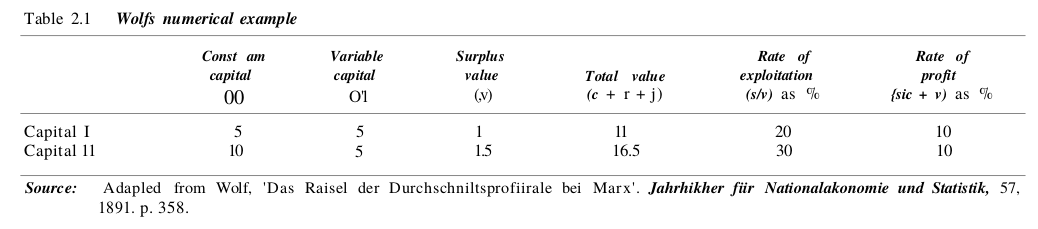
\includegraphics[scale=0.4]{wolfdata.png}
\caption{沃尔弗的数字例子}
\label{fig:wolfdata}
\end{figure}

沃尔弗认为“价值规律并没有被破坏”,在马克思那里不存在自相矛盾的地方。“恰恰相反,
它(解决方法)提供了一个新的证据,证明马克思对于资本主义经济的批判体系,是深刻且
富有远见的”沃尔弗的结论声称整个问题是个伪命题,这一混乱部分地是由恩格斯造成的,
恩格斯试图使先前解决这一问题的尝试都无效,并(沃尔弗隐晦地暗示)推迟了《资本论》
第三卷的出版。无论如何,和斯蒂贝林一样,沃尔弗是\textbf{回避}而不是解决这个问题。

更有意义的的贡献来自彼·法尔曼,施米特称其为“优秀的小伙子、移居美国的俄国犹太人、
职业化学家”。法尔曼受到李嘉图理论的强烈影响。他区分了商品价格中的两个因素:由物
化在商品中的劳动数量决定的商品价值的“\textbf{构成因素}”,以及代表资本家和地主对
产品份额索取权的“\textbf{分配因素}”。法尔曼主张,由于社会财富是由人们生产的商品
中所包含的人类劳动的总量构成的,因此,\textbf{总的来说,价值必须等于价格}:“两种
商品相交换时,一种商品的价格高于它的价值的大小,必然等于另一种商品的价格低于它的
价值的大小,反之亦然”,价格和价值之间差异的产生是\textbf{分配因素}造成的。

他也反对沃尔弗的结论,因为\textbf{沃尔弗认为价值量会随着劳动生产率的提高而增加,
  这和马克思的观点是矛盾的。}法尔曼非常清楚地说明了每个部门的价格、价值和资本有机
构成之间的关系:

\begin{quotation}
  如果利润是剩余价值的表现形式,怎么能够认为在剩余价值量取决于工人数量的同时,
  利润量似乎是独立于工人的数量的呢?仅仅因为,投资在生产资料上的资本和投资在工资
  上的资本之间的比率(或者像马克思说的那样,不变和可变资本之间的比率 $c:v$)最大的产
  业部门,其商品以高于它们价值的价格出售,这意味着,不变资本和可变资本的比率最小
  的产业部门,其商品以低于它们价值的价格出售,$c:v$ 的大小代表着明确的平均水平时,商
  品才按照它们的实际价值出售。
\end{quotation}

这同价值规律并不矛盾,因为总价格仍然等于总价值。个别商品的价格与价值之间的差异
只是竞争引起的波动造成的。“但是在严密的科学中,人们从来不把可精确计算的波动理解
为对规律的否定”。

法尔曼通过强调\textbf{总价格和总价值相等}(莱克西斯强调\textbf{总利润和总剩余价值
  相等})对莱克西斯的工作做出了补充,但是他对有机构成与价格和价值之间偏离关系的分
析更为严密一些。和莱克西斯不同,法尔曼用一个简单的数字例子讨论转形问题,同时对自
己的解决方法进行了一般化处理,以使之能够包含地租和利润的支付,但是这两点并没有被
很好地加以展开,法尔曼对利润率和所用资本关系的分析,表现的并不比施米特更好。

慕尼黑的教授莱尔博士反对沃尔弗的观点,沃尔弗认为,在马克思那里,生产率不同的劳动
创造出不同的价值。莱尔文章最重要的部分是他对转形问题的代数表述,这些代数表达式预
见到了后来德米特里耶夫和\textbf{(尤其是)博特凯维兹}的数学分析。

对整个经济而言,相应的加总分别为K, V和M,他采用了和马克思相同的立场,
用$M/(K+V)=r$ 表示平均利润率。“每单位商品的交换价值”用$t_1, t_2, \cdot $ 表
示(这事实上等同于博特凯维兹的价格—价值比率,即生产价格和劳动价值的比率)。

\begin{figure}
\centering
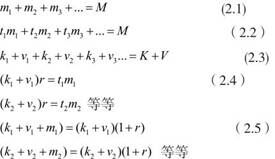
\includegraphics[scale=1]{laier.jpg}
\caption{莱尔的等式}
\label{fig:laier}
\end{figure}

等式(2.1)和(2.2)一起表示总利润等于总剩余价值。等式(2.3)纯粹是定义性的,而等
式(2.4)和(2.5)是试图把每个部门的剩余价值同利润,价值同生产价格联系起来的不成
功的尝试。\textbf{因为它们假定在单个部门内部,价值量和价格量是相等的,这样的假设
  是完全错误的。}……事实上,莱尔唯一直接的推论是\[t_1=t_2=t_3= \ldots = t_n=1 \]

\textbf{这个等式,只有在所有产业的资本有机构成相同的情况下才成立}。莱尔再次没有能够说明马
克思的原理,即$t_i$ 可能大于也可能小于单位值,因为不同产业的资本有机构成可能超过或
低于社会平均水平的资本有机构成,但是莱尔的确提供了一个隐含地表达了这种观点的算术
例子。

作为一个自称为“庸俗经济学家”的学者,莱尔对马克思的价值理论并不十分认同,不大可
能有太多的热情为马克思主要的分析性问题作出解答(虽然他在一定程度上是这样做了)。
莱尔的文章充满了对劳动价值论的批评,其中的一些内容有着强烈的现代说法。莱尔反对只
有在不存在技术进步的情况下,历史的物化劳动和实际的必要劳动才相等的观点,因为随着
时间的发展,技术进步降低了生产商品所需的劳动投入。\textbf{可供选择的其它生产方法
  的存在(比如使用肥力存在差异的土地)使得“必要劳动”的定义变得含糊不清;}无论是
直接地还是间接地,就维护人类生存的体系而言,几乎所有的人类活动都是必须的,因此从
资本主义社会整体的视角看,所有劳动都是必要的,不存在什么剩余劳动。

这些观点中,没有任何一个和转形问题直接相关,但它们的含义\textbf{远远超过了当代新
  古典主义对马克思的批判},并且他很早就预见到那些在斯拉法《\textbf{用商品生产商
  品}》出版后才出现的思考。很明显,莱尔是一个充满活力和原创性的马克思理论的批判者,
恩格斯和后来的马克思主义者对他的忽视实在令人难以理解。

\section{恩格斯的裁决}

恩格斯在为《资本论》第三卷撰写的序言中,用较大的篇幅对参赛者进行了评价。虽然他
没有颁发奖品,但是对莱克西斯、施米特和法尔曼进行了赞扬。莱克西斯是“一个伪装成庸
俗经济学家的马克思主义者”。“我们看到”,恩格斯对莱克西斯的文章评论道,“问题在
这里远没有得到解决,尽管已经含糊地、肤浅地,然而大体上正确地被提出来了”。恩格斯
认为,这已经是可能从莱克西斯那样背景的人那里得到的最多的东西了。法尔曼“实际上已
经接触到了问题的关键”,恩格斯说,“但是,他这篇如此重要的论文所受到的不应有的冷
遇却证明,……仍然需要有许多中间环节,才能完全地、明确地解决这个问题”。至于施米
特,他是第一个真正试图解决(与叙述相对)这一问题的人,但是他没有成功;认为剩余产
品价格的决定区别于不变资本和可变资本价格的决定,事实上等于抛弃了价值理论。施米特
发表在《新时代》上的论文同样是错误的。在恩格斯看来,施米特的真正成就是他分析利润
率下降趋势、商业利润、利息和地租的内容。

在恩格斯看来,沃尔弗只是愚弄了他自己。马克思在《资本论》第一卷有上百处,说的正是
和沃尔弗“解决方法”的基础相反的话。“\textbf{说什么马克思认为在可变资本减少时相
  对剩余价值的增加和不变资本的增加成正比,而这个断言令人如此吃惊,足以使一切议会
  辞令相形见绌}”。

\chapter{价值理论的第一次争论:1895-1914年}
\label{chap:1stzhenglun}

\section{《资本论》第三卷}

在《资本论》第一卷中,马克思简要提及了自由竞争的存在给其价值理论带来的难题。在
《资本论》第三卷第二篇,他对这个难题作了详细阐释,并提出了自己的解决方法。劳动力
市场的竞争造成\textbf{所有产业利润率的平均化},因为在均衡状态下,无论是工作日的长
度还是实际工资的大小都趋于一致,因此,资本家能够从每个雇佣工人那里榨取的剩余价值
量也将趋于相等。如果不同部门的资本有机构成不同——没有什么经济机制确保它必然相
同——它们就将有\textbf{不同的利润率}。产业 $i$ 的利润率被定义为剩余价值和使用的总
资本(不变资本加可变资本)之间的比率:$r_i=\frac{m_i}{c_i+v_i}$ ,把右边个分数的
分子和分母分别除以 $v_i$,得到 $r_i=\frac{m_i/v_i}{(c_i/v_i +
  v_i/v_i)}=\frac{e}{k_i+1}$ ,这里 $e(=m_i/v_i = m_j/v_j)$ 是\textbf{一般剥削
  率}, $k_i=\frac{c_i}{v_i}$是资本有机构成。\textbf{从而,资本有机构成低的产业,
  会有较高的利润率。但是,这与存在竞争的商品市场上的情况不一致,在竞争性商品市场
  中,资本可以从一个产业向另一个产业自由流动,所有生产部门的利润率将趋于平均化。
  因此,在价值规律和自由市场的运行之间存在明显的矛
  盾。}\pagescite[][159-172]{capital3}


在《资本论》第三卷中,马克思表明,要解决这种矛盾,需要对\textbf{劳动价值与长期均
  衡价格之间的有系统的偏离}作出清晰的认识。马克思把长期均衡价格称作\textbf{生产价
  格},他认为生产价格必须处于这样一种水平,即它必须能够包含资本家的成本和用当前的
平均利润率计算的资本家所用资本获得的利润。对个别资本家来说,由于剩余价值完全取决
于劳动中活劳动的数量,利润取决于使用的总资本(死劳动加活劳动),因此剩余价值和利
润也将发生背离。

\begin{quotation}
  就利润来说,不同的资本家在这里彼此只是作为一个股份公司的股东发生关系,在这
  个公司中,按每100资本均衡地分配一份利润。因此,对不同的资本家来说,他们的各份利
  润之所以有差别,只是因为每个人投在总企业中的资本量不等,因为每个人在总企业中的
  入股比例不等,因为每个人持有的股票数不等。\pagescite[][178]{capital3} 
\end{quotation}
 因此,\textbf{价值向价格的转化同时也是剩余价值向利润的转化}。

 资本论中 \pagescite[][174-176]{capital3}的数字例子,清楚地说明了转形问题包含的
 内容。五个部门分别投资100单位资本,每个部门有不同的资本有机构成和相同的剥削率
 ($e=100\%$)。无论是生产出的剩余价值总量还是利润率,和资本有机构成之间都是一种反
 向关系。

 然而,总的来看,\textbf{价格和价值是相等的}(等于442),同样\textbf{总利润也等于
   总剩余价值}(等于110)。这两个“不变条件”的重要性在于,它们使得平均利润率可以
 被定义为两个价值量之间的比率(总剩余价值除以使用的总资本)。马克思推论,一般利润
 率必须“从商品的价值引申出来,没有这种引申,一般利润率(从而商品的生产价格)就是
 一个没有意义、没有内容的概念”。\pagescite[][176]{capital3} 转形过程存在一
 个\textbf{历史的维度}。在\textbf{前资本主义社会}的商品生产中,生产者拥有自己的生
 产资料并相互交换他们的商品,劳动价值成为占统治地位的交换条件。从而
\begin{quotation}
  商品按照它们的\textbf{价值或接近于它们的价值}进行的交换,比那种按照它们
  的\textbf{生产价格}进行的交换,所要求的发展阶段要低得多。\textbf{按照它们的生产价格进行
  的交换,则需要资本主义的发展达到一定的高度。}\pagescite[][197]{capital3}

  因此,撇开价格和价格变动受价值规律支配不说,把商品价值看做不仅在理论上,而且在历
  史上先于生产价格,是完全恰当的。这适用于生产资料归劳动者所有的那种状
  态。\pagescite[][198]{capital3}
\end{quotation}

马克思设想,\textbf{利润率通过资本家之间的竞争而均等化},竞争首先在部门内部展开,
接着出现在部门之间,一般利润率只有到资本主义较晚的历史阶段才出现。

马克思对这个观点没有作进一步的论述,我们随后将会明白,他不这样做是明智的。除此之外,马克思留下了\textbf{另一个没有解决的难题}:
\begin{quotation}
  我们原先假定,一个商品的成本价格,等于该商品生产中所消费的各种商品的\textbf{价
    值}。但一个商品的\textbf{生产价格},对它的买者来说,就是\textbf{成本价格},因
  而可以作为成本价格加入另一个商品的价格形成。\textbf{因为生产价格可以偏离商品的
    价值},所以,一个商品的包含\textbf{另一个商品的这个生产价格内的成本价格},
  也可以高于或低于它的总价值中由加到它里面的生产资料的价值构成的部分。必须记住成
  本价格这个修正了的意义,因此,必须记住,如果在一个特殊生产部门把商品的成本价格
  看作和该商品生产中所消费的生产资料的价值相等,那就总可能有\textbf{误差}。对我们
  现在的研究来说,这一点没有进一步考察的必要。\pagescite[][184-185]{capital3}
\end{quotation}

比如,在表3.1中,五种商品中每一种商品的成本价格,都是按照用来生产这种商品的商品
(不变和可变资本)的\textbf{价值总和}来计算的。但是这些商品是按不同于它们的劳动价
值(特殊情况除外)的生产价格被出售的。然而,\textbf{马克思的“成本价格”完全不是
  价格},接下来的生产价格的计算也就不正确了。正如上述引文指出的那样,马克思发现了
这个困难,但却\textbf{没有提供任何解决它的方法。}

\section{对《资本论》第三卷的早期反应}
马克思对转形问题的分析存在两个重大的难题。假如价值规律在任何时候都可以直接应用,
而在某些情况下却不能发挥作用,这对价值规律的科学地位来说意味着什么?对于马克思在
自己的解决方法中已经意识到、但未能加以纠正的技术性缺陷,能够做些什么呢?恩格斯似
乎没有意识到第二个问题的重要性(参见以上第二章)。他被第一个问题深深地困扰着。他
在生命的最后几个月里,仍然就价值向价格转形的历史问题,同维尔纳·桑巴特和康拉德·施
米特保持着通信,并写下了一篇回复马克思批判者的长文(后来以《资本论》第三卷第二版
的增补发表)。事实上,这个增补成为恩格斯最后一篇重要的、专门研究价值理论的著
述,\textbf{这个增补也成为恩格斯对马克思主义理论最有原创性、也最具争议的贡献之
  一。}恩格斯对价值理论的关注表明,价值理论在所有流派的经济学中都处于十分重要的位
置,对马克思主义政治经济学来讲尤其如此,价值理论在马克思主义经济学对抗新古典学派
时发挥了核心作用。

维尔纳·桑巴特在对《资本论》第三卷的评论中,清楚地说明了价值向价格转形的历史问
题。桑巴特写道,马克思事实上是否打算像坚持价值理论在分析方面具有重要的意义那样,
坚持\textbf{价值理论的形成存在一个具体的历史过程},在《资本论》第三卷中并没有清晰
地展现出来。如果马克思的确有这种打算,那么\textbf{价值理论就包含了逻辑和经验两方
  面的错误}。桑巴特认为,\textbf{价值是一个纯粹的理论概念},它不必也不可能对应着
任何可观察的历史时期,任何试图以这种方式应用价值理论的尝试,都会发现它\textbf{和
  历史事实之间的矛盾}。早期的产业资本家是那些受到更高利润率吸引,并把他们商业资本
的一部分投资于制造业的商人。\textbf{如果在资本主义发展的早期阶段,商品是按照它们
  的劳动价值出售的,那么资本有机构成最低的产业将获得最高的利润率。但是,桑巴特指
  出,事实恰好相反,}资本主义生产关系首先出现在与活劳动使用相比,使用死劳动的比例
最高的产业(比如采矿业)。他认为,\textbf{当代资本主义经济中利润率和资本有机构成
  之间是一种反向变动关系的观点,同样是错误的。}事实上与此相反,高利润率存在于诸如
化工业、酿造业和采矿业等资本有机构成相对较高的产业。\textbf{资本主义产业利润率是
  由竞争的程度},而不是由不变资本和可变资本的比率决定的。因此,任何试图从价值向价
格转形的角度出发,构筑一个有关价格形成的历史理论,都将是完全错误的,转形问题是智
力活动的结晶,而不是现实生活中发生的事情。桑巴特指出,除非恩格斯使他相信相反的东
西,否则他将认为马克思持有和自己类似的观点。\textbf{桑巴特意思是,如果马克思能够
  活着自己准备出版《资本论》第三卷,就有可能消除这些不确定性。}

\textbf{勒克西斯}对马克思作了较多的批评,认为马克思对一般利润率形成的历史描述完全
站不住脚。\textbf{利润率的相等(除了偶然的例外)是资本主义生产的本质}。从来不存一
种社会条件,这种生产条件使得资本主义生产方式同由资本有机构成不同造成的利润率不等
同时并存。\textbf{利润率的相等等同于资本主义的生产方式}并同它们不可分割地联系在一
起。这很像在胚胎中,血液循环的发展等同于胚胎的形状与形式的发展。

康拉德·施米特肯定是了解桑巴特的批评的。……他告诉恩格斯,“价值规律(如果人们把它
当作调节交换的规律而不只是价值的定义)在我看来似乎只是一种虚构,尽管它本身自然不
会是错误的。恰恰相反,\textbf{它是一种必要的虚构},也就是说,它是我们为了得到除此
就无法获得结论而必须作出的一种假设”。就像恩格斯自己在《反杜林论》中表明的那样,
类似的必要的虚构在数学中经常出现。如果没有总价值等于总价格的虚构,将无法得出一般
利润率是由总剩余价值和总预付资本之间的比率决定的这一基本规律。

恩格斯回复施米特:
\begin{quotation}
  您在利润率问题上为什么走上了岔路,我认为,您的来信已经使我得到了一些解释。我在
  这里发现了同一种陷入枝节问题的偏向,我把它归咎于 1848年以来在德国大学中流行
  的\textbf{哲学研究的折中主义方法},这种方法丢掉了事物的总的概貌,过于经常地陷入
  一种几乎是无休止、无结果的\textbf{对枝节问题的思辨}中。

  您对价值规律的责难,从现实的观点来看,涉及\textbf{一切}概念。思维和存在的同一
  性(用黑格尔的话来说)完全符合于您举的圆和多边形的例子。换句话说,这两者,即一个事
  物的概念和它的现实,就像\textbf{两条渐近线}一样,一齐向前延伸,彼此不断接近,但是永
  远不会相交。两者的这种差别正好是这样一种差别,由于这种差别,\textbf{概念并不无条
    件地直接就是现实,而现实也不直接就是它自己的概念。}由于概念有概念的基本特性,就
  是说,它不是直接地、明显地符合于使它得以抽象出来的现实,因此,毕竟不能把它和虚构相
  提并论,除非您因为现实同一切思维成果的符合仅仅是非常间接的,而且也只是渐近线似地
  接近,就说这些思维成果都是虚构。

  一般利润率的情况不就是这样吗?它在任何时候都只是近似地存在着。它们全都没有任何其
  他的现实性,而只是一种近似值,一种趋势,一种平均数,但\textbf{不是直接的现实}。其所
  以如此,部分地是由于它们所起的作用被其他规律同时起的作用打乱了,而部分地也是由于
  它们作为概念的特性。(马恩文集,第10卷,P692-694)

  无论桑巴特还是施米特——至于那位大名鼎鼎的洛里亚,我在这里顺便提到他,只是把他当
  做逗人笑的庸俗经济学的陪衬——都没有充分注意到:这里所涉及的,不仅是纯粹的逻辑过
  程,而且是历史过程和对这个过程加以说明的思想反映,是对这个过程的内部联系的逻辑
  研究。\pagescite[][1013]{capital3} 
\end{quotation}
1895年春,恩格斯完成了名为“价值规律和利润率”的《资本论》第三卷的增补,在对洛
里亚进行回击后,恩格斯总结了桑巴特和施米特对价值概念逻辑地位的分析。无论是桑巴特
还是施米特,“都没有充分注意到:这里所涉及的,不仅是\textbf{纯粹的逻辑过程},而且
是\textbf{历史过程和对这个过程加以说明的思想反映},是对这个过程的\textbf{内部联系
  的逻辑研究}”。不可否认,马克思自己对这个问题的分析只是提供了一个粗略的大纲,毫
无疑问(恩格斯暗示),一旦有机会马克思将对此进行深入的扩充。恩格斯在“增补”的其
余部分中,对填补这个空白进行了大胆的、但最终被证明是难以令人信服的尝试。

…… 商人之间的竞争使\textbf{不同产业的利润率}平均化。后来,随着工厂生产的出
现,\textbf{不同部门的利润率}也被平均化了。这是通过“把一向阻碍资本从一个部门转移
到另一个部门的绝大部分\textbf{障碍清除掉}。这样,对整个交换来说,价值转化为生产价
格的过程就大致完成了”的时候实现的。进一步推动这个过程的事实是,“占有超额剩余价
值的各生产部门,也就是说,可变资本较多而不变资本较少,因而资本构成较低的各生产部
门,按照它们的性质来说,从属于资本主义的经营恰恰是最晚的,而且是最不充分
的;\textbf{首先是农业}”。

这是一个企图从劳动价值论的视角改写几千年经济史的雄心勃勃的尝试,这种尝试的失败并
不奇怪。现代批评者认为,\textbf{在前资本主义社会,商品生产从来就没有充分发展到按
  照商品的劳动价值比率相交换的程度}。重要的领域完全处于商品生产之外;很少有哪个交
易商专门把整个经济活动的时间用于商品的生产;劳动力的流动遇到的强大的体制和文化障
碍,阻止了单位资本收入的均等化;封建主义的剥削关系和商人资本从来就没有完全消失。
因此,除了可能在北美和澳大利亚的殖民地存在过一段短暂的时期外,\textbf{简单商品生
  产几乎从来就没有存在过。}

\section{庞巴维克和希法亭}
庞巴维克在1896年出版的著作中,对劳动价值论进行的新古典主义的攻击产生了较大的影响。
在国际上,无论是与门格尔还是与维塞尔相比,庞巴维克都更为知名,事实上,到世纪之交,
除了阿尔弗雷德·马歇尔,庞巴维克比任何他同时代的人都更加知名。庞巴维克是\textbf{主
  观价值论}的重要倡导者,但他充满原创性的独特的\textbf{利息理论}更广为人知,庞巴
维克用这一理论来取代马克思对资本主义利润的解释。庞巴维克认为,\textbf{资本的使用
  扩展了生产的时间结构},使得使用更加“\textbf{迂回}”的生产技术成为可能。由
此\textbf{导致的投入的使用和最终产出的出现之间的时间间隔的增加},既允许(通过提高
劳动生产率)也要求\textbf{利息的支付}(资本家对当前消费的偏好超过对未来消费的偏好,
在不存在回报的情况下,这会阻止储蓄的发生)。

在任何意义上,庞巴维克都不是一位天生的资本主义辩护者,但他的确在奥匈帝国的学术和
官方体制中,享有受人尊敬的地位。\textbf{他有关“迂回”生产的观点影响了杜冈-巴拉诺
  夫斯基和布哈林}(参见以下第十章和第十五章)。毫无疑问,他对马克思主义的兴趣,因
为与奥地利社会民主党日渐增加的影响作斗争的需要而得到进一步加强。早在1884年,他就
对《资本论》第一卷进行了猛烈的攻击,这是所有对马克思的\textbf{价值分析}进行的正统
批判中的第一次,也仍然是\textbf{最有说服力的一次}。他认为,无论是在演绎方法上,还
是在经验证据方面,劳动价值论都是难以成立的。正如马克思主张的那样,两种商品能够相
互交换,它们之中必然包含了一些共同属性。但是在考察商品交换条件时,马克思在抽象掉
商品的使用价值后,\textbf{错误地否定了效用也可以成为商品的共同属性}。这是一个“最
粗糙的逻辑错误”,\textbf{它混淆了从一般属性进行抽象和从这种一般属性的特殊形态进
  行抽象。}即使忽略掉使用价值,商品仍然存在许多其它与交换相联系的共同属性,比如商
品的\textbf{稀缺性}、它们都是供求的对象,都被私人占有,也都是自然的产物等等。

在庞巴维克看来,劳动价值论也无法被经验所证明。它不适用于那些不能自由地再生产出来
的商品(包括土地),也不适用于那些由熟练劳动生产出来的商品,《资本论》对熟练劳动
的分析是极其不充分的。\textbf{工资非常低的工人生产的商品有着非常低的价值}。此
外,\textbf{劳动价值论只适用于作为(如果成立的话)价格长期波动的中心。在短期内,
  供求占据支配地位。}最后,在1884年的著作中,庞巴维克暗示了后来广为人知
的\textbf{转形问题}——包含同样数量“社会平均劳动”的两种商品,会因为用来生产它们的
资本的耐久性的不同而有不同的价格。因此,价值理论“对于很大一部分商品是完全不,对
于其余的商品总是不、甚至是绝对不”适用的。劳动价值法则与一般价格法则的关系,就
同“\textbf{刮西风便下雨}”的法则与“\textbf{下雨}”的一般理论的关系一样。庞巴维
克清楚地表明马克思的分析同洛贝尔图斯的分析一样,存在的\textbf{主要缺陷就是“与事
  实相矛盾”,这种矛盾源自把“平均利润率规律”和可变资本是剩余价值的唯一源泉连接
  在一起。}马克思同洛贝尔图斯的不同之处在于,他承认了这个矛盾。“但是他犯下的仍然
是这个错误,而不是别的什么错误”。

十二年后,庞巴维克看到了《资本论》第三卷的解决方法……“我感到困惑,在这里,我看
到的不是对矛盾的解释和调和,而是赤裸裸地暴露了矛盾本身,马克思《资本论》第三卷同
第一卷是相矛盾的”。马克思提出的为劳动价值论进行辩护的四个论点,没有一个是令人满
意的。第一个论点(总价格等于总价值)与主题毫不相干,因为\textbf{价值理论涉及的是
  相对价格而不是绝对价格的决定问题}。第二个论点认为\textbf{价值规律支配价格}(而
不是价格水平)的运动,也是错误的。马克思证明的只是\textbf{劳动的量的变化是价格运
  动的一个原由,而不是物化劳动是价格运动的唯一决定因素。}庞巴维克\textbf{没有注意
  到}另一点,即由于\textbf{一般利润率}被认为是劳动价值的比率,\textbf{因此生产价
  格本身是由价值决定的。}一旦在物化劳动量保持\textbf{不变}的情况下,\textbf{工资
  的变化改变了均衡价格,马克思的第四个论点就崩溃了。}庞巴维克把第四点当成天大的难
事:对马克思来说,实际工资等于工人消费的工资商品中\textbf{由物化劳动量决定的劳动
  力的价值}。为了证明他对这一点的批判,庞巴维克需要对马克思工资理论作出正面攻击,
但是他并没有作这样的尝试。

庞巴维克对马克思第三个论点——和\textbf{价值转化为生产价格的历史过程}有关——的驳斥更
有说服力。他认为,马克思在这一点上有点想当然,马克思说明了在应用劳动价值论时交换
是如何进行的,但却没有解释为什么会如此。事实上,庞巴维克坚持认为,没有什么理由能
够说明它应当如此。从本质上看,“对生产者来说,\textbf{什么时候获得他们活动的回报},
是完全无关紧要的”说法,是令人难以置信的。恰恰相反,\textbf{工作的开始和最终产品
  的完成之间经历的时间的长短,是价格决定的一个重要因素,即使是在前资本主义社会也
  是如此。}马克思的观点被历史经验所否定,历史经验表明农民和工匠的收入,实际上受到
他们使用的资本数量的影响。庞巴维克引用桑巴特观点,说明资本主义生产首先出现在有较
高(而不是较低)资本有机构成、相对有着较低(而不是较高)利润率的产业部门。没有任
何证据表明,资本正在从这些产业流出,以寻求更高的利润。这些部门的增长速度实际上要
高于平均水平。

\textbf{桑巴特}通过把价值描述为一个\textbf{逻辑范畴而不是经验范畴}为劳动价值论辩
护。庞巴维克认为这不会令马克思感到满意,\textbf{因为对马克思来说,价值的确是“一
  种真实世界的存在,而不只是思想的构建”。}然而,结论必然就是,劳动价值论从来就没
有被应用过,即使是在原始社会也是如此。这就意味着,马克思主义整个体系,与在它之前
的黑格尔体系一样,是“纸牌堆成的房子”。

1904年,庞巴维克的观点公开出版8年之后,鲁道夫·希法亭对庞巴维克的批判作了唯一一次
系统的、马克思主义的答复。希法亭的反批判由两部分构成,一部分是\textbf{方法论}的,
一部分是\textbf{历史}的。但是,在这两部分中,\textbf{没有任何一部分涉及庞巴维克提
  出来用以反对劳动价值论的具体详细的批评}。这如同后来发生在许多马克思主义政治经济
学领域的争论一样,参与争论的\textbf{双方都未能深入地了解对方的论点,而且缺乏真正
  的对话。}在更为一般性的哲学层面上,希法亭指责庞巴维克总是把\textbf{自然现象和社
  会现象混为一谈}。
\begin{quotation}
  每一种从使用价值出发的价值理论,也就是说从事物的\textbf{自然属性}出发的价值
  理论……是从\textbf{物与人的个别关系}而不是从\textbf{人们之间相互的社会关系}出
  发……这种视角是\textbf{非历史的和非社会的}。它的范畴是自然的和永恒的。
\end{quotation}

劳动价值论不只是,甚至\textbf{不主要是对价格决定的分析}。“正是因为劳动是把分裂为
各个原子的社会联结起来的\textbf{社会纽带},\textbf{而不是因为劳动是技术上最有意义
  的东西},劳动才成为具有现实意义的价值的原则,价值规律才具有现实性”。\textbf{马
  克思的价值论和主观价值论之间的根本区别,远不像庞巴维克认为的那样,只是两种方法
  (可以想象两种方法之间存在互补关系)之间的区别。}这种区别更像是“\textbf{互相竞
  争和互相排斥的观察整个社会生活的视角}”之间的区别。资产阶级经济学的个人主义带来
的完全是\textbf{政治经济学的自杀}。10年后,布哈林雄辩地重新表述了上述对新古典理论
的方法论的批判,并试图表明新古典主义的视角反映了新的“有闲阶级”的观点,这一新阶
级是随着金融资本的兴起而产生的。

在希法亭看来,世界观上的差异和价值转化为生产价格的历史过程紧密相关。在马克思的著
作中,“\textbf{概念的发展完全同历史的发展相平行},因为在马克思主义体系中,社会生
产力的发展,一方面表现为历史现实,另一方面也在概念中得到反映。而且这种平行发展同
时也为理论的正确性提供了最严格的经验证明庞巴维克对劳动价值论在简单商品生产中的适
用性的反对,是没有根据的。因为农民和工匠不可能在不同产业之间自由的流动,利润率的
差异与他们无关。在任何情况下,庞巴维克的分析中提到的资本有机构成之间的重大差异,
指的都是\textbf{资本主义而不是前资本主义经济},这表明庞巴维克的观点是完全无效的。
资本主义工商业中最早出现的有机构成较高的部门,吸引了商人向产业生产的转移,是因
为\textbf{“合法的和事实上的垄断”力量},使得他们能够以高于他们劳动价值的价格出售
他们的商品。在希法亭(把注意力转向了桑巴特)看来,事情的发展顺序如下:商业资本家
开始在制造业中使用他们 “过剩的资本”,然而他们仍然主要是商人。他们从产出数量的增
加和生产规律性的提高,从他们有能力占有工匠生产出来的剩余价值的一部分中获益。“即
使是他们能够保证的,投资在产业中的资本的利润率低于他们可以获得的商业资本的利润率,
然而自此以后他们的总利润仍然是增大了”。最后,资本家进一步从\textbf{更加先进的生
  产方法}中获益,尤其是当特殊的法律赋予他们独占新技术的权利时。“\textbf{直到垄断终结的那
一天……最初极不相同的利润率才有可能平均化}”。竞争首先使个别生产领域的利润率平均
化,随后,资本从一个生产领域向另一个生产领域的自由流动,为整个经济确立了统一的利
润率。

庞巴维克对希法亭的答复完全无动于衷。奇怪的是,希法亭和庞巴维克\textbf{都没有讨论
  马克思转形问题解决方法中存在的技术性难题},合理的推断只能是他们没有注意到这些问
题。希法亭偶尔提及这些问题,表明问题本身并没有激起他足够的信心,使他觉得自己有能
力去解决它们。希法亭\textbf{强调总价值和总价格相等}的重要性,这种相等表明,“所有
的利润都源自生产,而不是来自后来资本家对最终产品产生的任何影响”,希法亭接着给出
了一个大胆的但不合逻辑的断言:“既然总价格等于总价值,那么总利润除了是总剩余价值,
不可能是其他什么东西”。事实上,马克思已经指出了这一点,但是它还没有得到证明。接
下来,希法亭从无根据的断言转向了完全的错误,他宣称,马克思主要关注的是\textbf{工
  资和利润之间的比率},“因此[原文如此]说在关注个别商品时马克思放弃了价值规律,而
只在考察这些商品的总体时才坚持价值规律的有效性,是完全错误的”。希法亭在这里提示
的\textbf{似乎是剥削率与利润和工资之间比率的相等。这是一种妄想}。就像在下一节将要
看到的那样,在一般情况下,马克思的\textbf{两个“不变条件”只有一个能成立}。如希法
亭提示的第三个条件的成立,只能以牺牲上述两个“不变条件”中的一个(或者更有可能同
时牺牲两个)为代价。

争论双方没有任何一方在交流中变得更为完善。庞巴维克对《资本论》第三卷的批评明显不
如他对第一卷的批评。尤其是\textbf{他未能正视马克思劳动价值逻辑优先性的主张},正视
这个主张,就要对马克思一般利润率能够用(且只能用)价值比率加以确定的观点进行反驳。
这反过来对庞巴维克也提出了新要求,他需要对马克思的技术分析,作出比他原本认为的更
多的研究性评价。

\section{米尔普福特和德米特里耶夫}
东普鲁士哥尼斯堡的沃尔夫冈·米尔普福特的社会主义是俾斯麦式的而不是马克思主义
的……米尔普福特的论文和文章,包含两个存在细微差别的\textbf{转形问题的代数表达},
并且非常清晰地指向了20世纪50年代和60年代有关转形问题的数学文献。马克思没有把投入
的\textbf{不变资本和可变资本转化为生产价格},米尔普福特以此为出发点,认为这个问题
可以运用下述方式解决。用 $a_1$ 表示商品1的劳动价值,$x_1a_1$ 表示它的生产价
格,$x_1$ 是价格与价值的比率,这意味着价格是由劳动价值度量的。$p$ 表示一般利润
率,$x_0$ 被定义为 $1 /(1+p)$,马克思意义上商品1的“成本价格”(米尔普福特把它命
名为公司1的“资本价格”)由 $x_0x_1a_1$ 给出。对n个生产不同商品的企业来
说,$a_{11},a_{12},\cdots,a_{1n}$ 是为了生产\textbf{一单位商品}1使用的商
品 $1,2,\cdots,n$的数量;$a_{21}$同理等等。用现代术语来说,它们就是每个产业
的\textbf{里昂惕夫投入系数}。米尔普福特明确地表明,它们是由“各个公司的技术”决定
的。然后,他写下了下列等式:
\begin{gather}
  x_0a_1x_1=a_{11}a_1x_1 + a_{12}a_2x_2 + \cdots  \notag \\
  x_0a_2x_2=a_{21}a_1x_1 + a_{22}a_2x_2 + \cdots \notag \\
  \cdots \cdots \cdots \cdots \notag \\ 
  x_0a_nx_n=a_{n1}a_1x_1 + a_{n2}a_2x_2 + \cdots 
\end{gather}
在上面的式子中,左边给出了每单位不同商品的成本价格,右边是生产它所需的不同商品单
位投入的价格总和。米尔普福特在一定程度上和马克思一样,\textbf{忽视了不变资本和可
  变资本的区别,把工人消费的商品看作是和原材料与机器一样的物质投入。}这是一个在有
关转形问题的现代数学讨论中经常出现的情况,而且很容易被改进为一个更加正统的马克思
的表述式。

米尔普福特得到了n个等式,但是却有$n+1$个未知数(n个价格与价值的比
率 $x1......xn$和用 $x_0$ 表示的利润率),在这一点上他泄气了。他可以做的是,要么
使所有商品的价值总和等于价格总和,要么使总剩余价值等于总利润,得到第$n+1$个等式。
在这两种情况下,他都需要指定第n种商品的产出数量。他未能这样做,而且混淆了马克思的
两个不变条件,把$\sum a=\sum \pi $( $\sum \pi $ 代表\textbf{生产价格总和})写
为:
\begin{gather}
  (a_1 - a_{11}a_1 - \cdots - a_{1n}a_n) + \cdots + (a_n - a_{n1}a_1 - \cdots -
  a_{nn}a_n) = \notag \\
  (a_1x_1 - a_{11}a_1x_1 - \cdots) + \cdots + (a_nx_n - a_{1n}a_nx_n - \cdots)
\end{gather}
这真是\textbf{不伦不类}。左边代表了物化在\textbf{每单位}不同商品中剩余劳动的总量,
右边代表的是与\textbf{每单位}产出相对应的利润。\textbf{这个等式更加近似于第二个不
  变条件(总剩余价值等于总利润)而不是第一个不变条件。}正因为如此,米尔普福特才不
得不用\textbf{产出的数量}去乘以每单位产出的剩余价值和利润。如果
用 $X_1,X_2\cdots, X_n$ 表示商品$1,2 \cdots n$的产出数量,我们可以把:
\begin{gather}
  (a_1 - a_{11}a_1 - \cdots - a_{1n}a_n)X_1 + \cdots + (a_n - a_{n1}a_1 - \cdots -
  a_{nn}a_n)X_n = \notag \\
  (a_1x_1 - a_{11}a_1x_1 - \cdots)X_1 + \cdots + (a_nx_n - a_{1n}a_nx_n - \cdots)X_n
  \end{gather}
当作(真正的)总剩余价值等于总利润的条件。

即使是这样,米尔普福特的代数方法也是失败的,但是他的贡献不仅独具匠心,而且富有成
效,这一点是不可否认的。米尔普福特认为自己是在推动\textbf{古典价值理论和奥地利学
  派边际效用分析的综合},前者解释了\textbf{“自然”(即长期均衡)价格},后者
用\textbf{心理规律说明了稀缺性对短期价格决定的影响}。虽然存在一定的局限性,但奥地
利学派的理论仍然是现有的最佳理论。“从另一方面看,奥地利学派的错误在于试图把他们
的解释方法,应用于自由竞争条件下可自由再生产的商品的自然价格。我的观点是,在古典
学派和奥地利学派之间不存在不可调和的矛盾,这两个体系可以以一种我已经解释了的方式
统一在一起”。

V·K·德米特里耶夫(1868-1913)是当时最重要的俄罗斯数理经济学家。追随着同胞彼得·司徒
卢威和杜冈-巴拉诺夫斯基(参见以下第九章和第十章)的足迹,德米特里耶夫希望能够综合
古典与新古典主义的价值理论。虽然从来没有提到马克思,而且他著作中的大部分内容应归
功于\textbf{瓦尔拉斯}而不是李嘉图,但德米特里耶夫提供了一个\textbf{分析框架},这
个框架\textbf{对后来的劳动价值论和转形问题研究具有巨大的价值。}……论文认为劳动价
值的计算可直接从\textbf{物质投入和产出的技术数据}(马克思经常用其它的价
值——c,v,m——表达价值,从来没有明确地考虑过这个问题)得出。对于商品$A$,$N_A$表示它的
价值(即生产它所需的直接或间接劳动投入的总和);$1/m_i$是生产商品A耗费的第i种商品
的数量,或者,如果第i种商品是机器的话,它表示\textbf{年折旧系数};$n_A$是生产A的
直接劳动投入,德米特里耶夫得到:
\begin{gather}
  N_A = n_A + 1/m_1 N_1 + \cdots + 1/m_MN_M
\end{gather}
\textbf{在这里,劳动价值由直接劳动($n_A$)和间接劳动($1/m_1 N_1+\cdots$)的总和
  决定。}

德米特里耶夫也思考了\textbf{生产价格的决定问题}。然而,他的方法是\textbf{李嘉
  图}式的而不是马克思式的。他\textbf{使用“过去劳动”模型取代了不变和可变资本之间
  的区分}。在这种模型里,不再把商品看作是由直接劳动和生产资料的结合生产出来的,生
产技术被“简化”为由它们作出贡献的时期加以区分的一系列劳动投入。棉纱被认为是纺纱
工的劳动(当年耗费的)、棉花种植者的劳动(去年耗费的)和必要的机器制造者的劳动。
棉纱由此可追溯到两年或更长时间的劳动。忽略掉机器,假定棉花是由不借助外力的劳动者
种植,那我们可以得到原棉和棉纱的“\textbf{过去劳动}”价格方程:
\begin{align}
  P_A &= WL_A(1 + r) \\
  P_B &= WL_B(1 + r) + W\frac{1}{m_A}(1+r)^2
\end{align}
$P_A, P_B$是棉花和棉纱的价格,$L_A, L_B$是种棉花和纺纱活动中每单位产出使用的劳动
的数量;$1/m_A$(再一次)是生产一单位棉纱要求的棉花投入的数量;$r$是年利润率。
则$L_A,L_B$和$(1/m_A)L_A$表示“过去劳动”,每个都被(1+r)的乘方加权,乘方的大小由
劳动被“锁定”在生产中的\textbf{周期的长短}决定。长期均衡价格,定义为资本家过去的
所有工资开支,加上包含所有相关时期以当前的平均利润率为折算系数计算出的复利形式
的利润的总和。简单地说,假定工人只消费谷物,给定时期资本家的支出为$n_AaP_A$ ,
$a$ 是每个时期工人消费的谷物的数量,$P_A$ 是谷物的价格。,$n_A$和前面相同,代表所
需的(这次是在时期A)直接劳动投入。对商品A(谷物)来说,自然价格(生产价格)被定
义为:
\begin{gather}
  P_A = n_AaP_A(1+r)^{t_{A1}} + \cdots + n_MaP_A(1+r)^{t_{AM}}
\end{gather}

r为平均利润率,在得到最终产品之前,劳动投入$n_A \cdots n_M$存在的生产周期
为$t_{A1} \cdots t_{AM}$ 。给定真实工资a,一旦定义了价格计量单位,便可由方程所代
表的方程组解出用技术系数$n_A \cdots n_M$ 与$t_{A1} \cdots t_{AM}$表示的生产价
格$P_A \cdots P_M$和 $r$。这甚至超越了米尔普福特,德米特里耶夫在19世纪的最后十年,
已经预见到了20世纪中叶出现的\textbf{数理经济学}。

\section{冯·博特凯维茨的解决方法}
上述这一切,都没有给西方的社会主义者留下什么印象,也没有对俄国的正统马克思主义者
产生什么影响。然而,德米特里耶夫的著作被有着俄罗斯血统的柏林统计学家拉迪斯劳
斯·冯·博特凯维茨注意到了。博特凯维茨是一个对马克思有着强烈兴趣的李嘉图主义
者……“正如马克思那样,德米特里耶夫的模型,把商品生产的技术条件,包括表现为给定
的实际工资的劳动力商品生产的技术条件,作为价格最终的和唯一的决定因
素”。\textbf{博特凯维茨用德米特里耶夫的代数框架,得出了马克思的剥削率和利润率函
  数(用“过去劳动”数量表示)。}他还说明,在作为货币的商品的有机构成、劳动力价值
和相关产业的生产价格之间存在精确的关系。

然而,马克思和德米特里耶夫之间也存在着重要的区别。博特凯维茨注意到,后者拒绝了马
克思在不变资本和可变资本之间所做的区分,并用代数表达式取代了数字例子。这种区别,
比它们表面上看起来要重要的多,因为它意味着一种重大的方法论上的突破:德米特里耶夫
使用\textbf{同时决定}的方式进行论证,而马克思使用\textbf{因果链条}进行推理,博特
凯维茨批评马克思这种推理是一种“\textbf{连续近似}”的谬误。德米特里耶夫证明了马克
思对李嘉图的批判是无效的,\textbf{李嘉图没有混淆价格和价值,也不需要马克思对不变
  资本和可变资本进行的区分,}李嘉图的主张(被马克思否定的),\textbf{利润率不受某
  些产业生产条件变化的影响},这些产业\textbf{既不生产工资商品也不生产用于(直接或
  间接的)工资商品产业的生产资料,这是正确的。}博特凯维茨在结论中,对马克思进行了
严厉的批判。“毕竟价值计算和价格计算之间有着密切的数学联系,马克思在这个问题上的
分析缺陷,反映了他数学能力的缺乏”。\textbf{马克思认为与价格决定相比,价值决定具
  有逻辑上的优先性是错误的}:“不仅价格、工资和利润率之间的相互关系,可以简化为无
需从价值和剩余价值的数量开始的数学表达式,而且如果使用正确的公式表达的
话,\textbf{价值和剩余价值的数量甚至可以不出现在计算中}”。

博特凯维茨似乎对马克思有些着迷,他的第二篇文章更为直接地分析了《资本论》第三卷中
的转形问题。从概念层次看,这篇文章不如第一篇成熟,\textbf{用三部类模型取代了存
  在n种商品的模型}(另外,对三个部类而言,生产不变资本的产业的\textbf{资本有机构
  成是相同的})。第\Rnum{1} 部类生产生产资料,第\Rnum{2} 部类的产出由工资商品构成,
第\Rnum{3} 部类生产资本家消费的奢侈品。博特凯维茨进一步抽象掉固定资本,所有的资本
每年周转一次,并假定\textbf{简单再生产}居于支配地位。这使得:
\begin{gather}
  c_1+v_1+m_1=c_1+c_2+c_3=C \notag \\
  c_2+v_2+m_2=v_1+v_2+v_3=V \notag \\
  c_3+v_3+m_3=m_1+m_2+m_3=M 
\end{gather}

在这里,不变资本的产出完全等于各个产业使用的不变资本;工资商品的产出正好足以养活
三个部类中的雇佣工人,奢侈品的产出正好等于生产的剩余价值的总量。同米尔普福特一样,
博特凯维茨用$p$表示平均利润率。另外,\textbf{$x, y, z$分别表示三个部类中生产价格
  和价值的比率};这和米尔普福特的$x_1 \cdots x_n$相对应。马克思的转形问题解决方法
要求:
\begin{gather}
  (c_1x+v_1y)(1+p)=(c_1+c_2+c_3)x \notag \\
  (c_2x+v_2y)(1+p)=(v_1+v_2+v_3)y \notag \\
  (c_3x+v_3y)(1+p)=(m_1+m_2+m_3)z
\end{gather}
等式(3.9)是米尔普福特的等式(3.1)在三部门模型中的对等物。等式左边代表(用价格
术语)每个部类的成本价格,乘以(1+p)表明生产价格必须包含成本和利润。右边表示用生产
价格而不是用劳动价值标示的每一类商品的产出。资本家必须从出售他们的商品中获得足够
多的收入(等式的右边)去补偿他们的支出和平均利润率为p时可获得的利润(等式左边)。

博特凯维茨有了(3.9)所表示的三个等式,但却有四个未知数:x, y, z和p。他注意到,那
个缺失的等式可以通过引入马克思两个“不变条件”中的任何一个得到(\textbf{但不是同
  时引入两个})。总价值和总价格的相等使得:
\begin{gather}
  Cx + Vy + Mz = C+V+M
\end{gather}

C, V和M是总量指标,使总剩余价值等于总利润等同于指定
\begin{gather}
  z = 1
\end{gather}
等式(3.10)和(3.11)表达了马克思的两个不变条件。如同博特凯维茨在几个数字例子中
表明的那样,\textbf{一般情况下,两个条件不可能同时成立。}比如,\textbf{在一个
  第\Rnum{3} 部类的资本有机构成低于社会平均构成的模型中采用等式(3.11),将使得价
  格总和超过价值总和,反之亦然。马克思假定是错误的。}只有那些生产工资商品的产业
(直接的或间接的)——事实上,即第\Rnum{1} 部类和第\Rnum{2} 部类,但不包括
第\Rnum{3} 部类——决定了利润率。在这一点上李嘉图是正确的,错误的是马克思。但是,博
特凯维茨提醒道,这种结论不能被推广的太远。这并不意味着部类\Rnum{3} 的资本有机构成
可以无限的大,因为如果它的确很大,那么利润率的均等化将不再可能。\textbf{马克思的
  分析存在问题,但他的本意是正确的。}

博特凯维茨的著作没有产生明显的直接影响。1949年,他的著作的英文翻译者保罗·斯威齐认
为,“有证据表明,它只被少数几个专家阅读过”。斯威齐没有对这些专家的身份进行说明,
就我们所知,1942年出版的斯威齐的《资本主义发展论》,对博特凯维茨的第二篇文章进行
了概括,并引发了对转形问题重要的(和持续的)争论,在此之前,对转形问题进行的认真
分析仅有两次。没有任何一个第二国际的著名理论家关注过这个问题。35年的空白期,折射
出这一时期马克思主义政治经济学科研水平的不足。在这一段暂歇期,对价值理论进行的哲
学思考出现了一些重大的进展,但有关这个问题的技术分析没有取得什么明显发展。直到线
性经济学工具在冯·诺依曼和里昂惕夫的著作(20世纪30年代和40年代)中出现后,对价值问
题“数量方面”的讨论才重新开始。

\chapter{伯恩施坦,考茨基和修正主义论战}

\section{德国社会主义的兴起}
19世纪后半叶,德国经济经历了特别高速的发展,帝国(1871年才成为一个政治统一体)由一个相对落后的主要农业区,转变为世界上重要的工业力量之一。……


与英国相比,德国的工业很大程度上受银行资助,银行获得了大量的股份和对制造能力方面
的控制权。德国银行业高度集中,到1914年,\textbf{五个最大的银行集团控制了全部银行
  资本的四分之三的份额。因而银行鼓励对价格操纵的卡特尔的形成,}卡特尔存在于世纪之
交的大多数产业中,促进了产业集中趋势的进一步发展。它们在海外的活动得到扩大,以至
于在19世纪80年代,德国已经成为\textbf{净资本输出国}。30年后,帝国的资产总计
达300亿马克,三倍于全国的年出口收入。在德国进行工业化的最初几十年里,贸易壁垒逐步
降低,直到遇到开始于1873年的严重萧条,这时候,来自北美的谷物和英国的生铁引起的竞
争,迫使大企业和容克都要求政府进行干预。1880年后,德国的市场再次受到\textbf{关税
  保护}。这只是国家普遍并越来越深入地参与经济活动的一个方面,这种参与还包括政府或
市政拥有铁路、矿山、工厂和公共设施的所有权,还包括\textbf{俾斯麦式的社会立法},这
些法律要求为疾病、意外事故和养老提供强制性的保险,对妇女、儿童的工作时间进行控制。
到1914年,德国已成为一个有着\textbf{强大社团主义因素的混合经济}。

帝国的社会结构密切地反映了它的经济基础。除大企业和工厂的无产阶级外,还存在一个
代表强大的准封建利益的地主;一个只能算是半无产阶级的且深受压迫的重要的农业工人阶
级;一个数量巨大、通常比较富裕的农民阶级,这个阶级在德国的南部和西部尤为明显;一
个经常变化的,由各种类型的城市商人、手工业者和小雇主构成的中产阶级下层。从政治和
文化方面看,\textbf{德国处于完全发展的资产阶级社会和旧体制的中间地带},前者的典型
代表是美国,后者的典型例子是罗曼诺夫专制政体。特别是在普鲁士,前资本主义制度以及
与之相适应的价值观念和行为方式仍然占主导地位,即使是在非常先进的资本家圈子里也是
如此。土地财富、军队和宫廷仍然拥有远远超过马克思主义理论家们认为的影响力。

当时德国的中层和上层阶级的观念非常保守,而且具有强烈的\textbf{民族主义倾向},既没
有同时代法国存在的反教权的激进的共和主义,也没有格莱斯顿时期英国兼容并包的自由主
义。上层资产阶级已经同贵族统治阶级结盟。同欧洲其他许多地方一样,贵族统治者的世界
观占据主导地位。雇主几乎普遍地敌视工会,这更多的是由于担心被颠覆,而不是由于对劳
动力自由贸易教条式的坚持。英国模式中存在的集体谈判和工业调解,在德国发展的非常缓
慢。在受人尊敬的德国政坛谱系的最左端,站的是“教授社会主义者”(讲坛社会主义者)。
像古斯塔法·冯·施穆勒和阿道夫·瓦格纳这些人,更多受到的是洛贝尔图斯的而不是马克思的
影响,试图把对不受约束的资本主义竞争的怀疑、对福利立法的支持,对德国政府以及德国
正在迅速发展的军事机器毫无异议的忠诚结合起来。

德国社会主义深深扎根在这片明显贫瘠的土地上。1875年,在哥达统一会议上,成立
了SPD——众所周知的德国社会民主党(the Social Democratic Party of Germany)的缩
写,SPD的成立是以一个马克思对它进行过严厉的批评、存在着一定程度的混乱和折中的纲领
为基础的。德国社会民主党无论在人数上还是在影响力上,都得到极为迅速的发展。三年后,
带有压制性的“反社会主义者非常法”没有影响社会民主党的选举活动,只是使党的宣传活
动变得更加复杂,但没有完全阻止党的宣传活动。SPD同迅速扩大的“自由”(非教派的,独
立于雇主的)工会建立了密切的联系,为了广泛地开展党的宣传工作,组建了一支庞大的由
付薪雇员组成的队伍,这支队伍中包括一些组织者、讲演者和新闻记者。到1914年,SPD的成
员已超过1百万,和它有联系的工会会员超过250万。在1912年的选举中,人口在1万或1万以
上的城镇中,SPD差不多赢得了接近一半的选票。当时,完全有理由相信,德国社会民主党会
取得更大的成功。德国社会民主党吸引了来自奥匈帝国、俄国以及德国国内的激进分子。它
的辩论受到密切的关注,它的纲领被深入研究,它的知识分子受到越来越多的尊重,在欧洲
内外都是如此。

总之,德国社会民主党是国际社会主义运动皇冠上的明珠,\textbf{是当时世界上最大的和
  最重要的马克思主义政党。}无论是在实践方面,还是在意识形态方面,它对第二国际都起
着主导作用。

\section{正统马克思主义和《爱尔福特纲领》}

考茨基负责被视为“正统”马克思主义的社会主义理论文献的制订和传播工作,在这一点
上,考茨基的贡献甚至比恩格斯还要大。这里谈到的“\textbf{正统}”马克思主义,同马克
思本人的思想相比,出现了\textbf{两个微妙但却是根本性的变化}。第一,作为马克思早期
著作的特点,并在马克思晚年某些著作中仍然保留的\textbf{黑格尔主义和人道主义的特征},
在很大程度上\textbf{被更为常见的实证主义方法所取代},资产阶级在对当时资本主义社会
的批判中广泛接受了实证主义方法。\textbf{严格的因果逻辑、趋势预测和决定论,逐渐脱
  离了马克思的辩证的先验论的范畴。}第二,\textbf{进化论的科学的自然主义被引进马克
  思的思想,随之而来的是有关国际和平、社会经济进步和科学认识日渐进步的乐观信念。}特
别需要注意的是,卡尔·考茨基在成为马克思主义者之前是一个达尔文主义者,他的哲学观点
更多受到的是《\textbf{反杜林论}》的而不是马克思早期著作的影响。考茨基把马克思主义
看作是\textbf{历史科学},他自己的马克思主义政治经济学牢固地建立在这一基础之上。

党开始考虑用一个新的原则声明取代难以令人满意的哥达纲领。新宣言中有关实践的部分,
交由德国社会民主党的议会领袖奥古斯特·倍倍尔和伯恩施坦负责,根据恩格斯的指示,考茨
基负责理论部分。最终形成的《爱尔福特纲领》指出:资本主义必然导致生产者的生产资料
被剥夺,小企业被大企业取代,由农民与小资产阶级构成的中间阶层将最终消失;技术进步
的一切利益都被资本家和地主独享,同时工人遭受苦难和无保障不断增长;阶级对立日益尖
锐;经济危机进一步加剧了这种对立,经济危机的根源在于资本主义生产方式的本质,经济
危机一天比一天扩大,越来越具有毁灭性;只有通过无产阶级协调一致的政治行动废除私有
制,才可能使人类的生产力得到充分的发展。

1892年,考茨基在他的著作《阶级斗争》中对纲领进行了系统的辩护,《阶级斗争》对资本
集中和经济危机的原因作了极为详细的说明。考茨基论证道,\textbf{资本集中和经济危机
  这两种现象密切相关。}信用不只是一种资本集中、剥夺非资本主义部分的人口、促进经济
快速发展的手段。它也是一种“使现代生产方式变得日益复杂并对一切干扰日益敏感的机体,
使资本家日益感到不安并使他们的活动基础愈加不稳”的手段。\textbf{危机是生产过剩的
  结果},而这种生产过剩是由资本主义生产的\textbf{无计划性}造成的。经济扩张的越快,
需求预则就变得越困难,市场条件的不确定性就越大,投机也就越疯狂。托拉斯和辛迪加无
法消除危机,无法阻止国际竞争,它们只能造成\textbf{资本家敌对集团之间“你死我活的
  斗争”}。

考茨基把资本主义生产的无政府状态解释成经济危机的原因之一,而日益增长
的\textbf{需求不足}是他分析危机产生的另一个原因。利润率下降趋势以一种\textbf{间接
  的方式}对危机产生冲击。……“\textbf{利润和利息的下降并不是资本家阶级的灭亡,而
  只是它的范围的缩小}”。反过来,这又成为生产过剩危机的一个重要因素,因为资本集中
以及它所推动的剩余价值的再分配,使得剩余价值开始从消费收入比大的小资本家向消费收
入比相对较小的大资本家转移。工人阶级消费的增长因失业率的上升而受到限制。

考茨基认为,结果将是长期的生产过剩和比以往任何时候都更加频繁、更加猛烈的危机。
从长期来看,国内需求的不足,无法由市场出口的扩大相抵消。因为最有利可图的市场已得
到充分的利用,剩下的尚未开辟的是那些“除了热带病和挨一顿棍棒之外,什么也得不
到”的市场。此外,资本主义生产在世界上迄今为止仍不发达的地区开始出现,通过创造自
己的竞争对手,“资本主义大生产为自己挖掘了坟墓”。市场的扩张最终将不再可能,
这“将意味着整个资本主义体系的崩溃”,它也已经“开始在自己的剩余中窒息”。考茨基
的推论是,资本主义将完成它的历史使命,未来的社会主义共和国取代资本主义的时机已经
成熟(这个主题,成为他这部著作下半部分的主要内容)。

《阶级斗争》用简单而形象的语言写就,坚持认为\textbf{迫在眉睫的社会变革即将来临},
成为一本具有重大影响的著作。除了恩格斯偶尔作出的思考(许多最重要的思考是三年后
《资本论》第三卷出版时才作出的),《阶级斗争》是唯一一次把马克思主义政治经济学
和19世纪90年代的实际情况相结合的认真尝试。至少在当时,这本著作的不足之处被掩盖
了……但是《阶级斗争》中的缺陷确实存在,无论是从经验上还是从理论上看,《阶级斗争》
都不能算是一本令人信服的著作。考茨基有关资本集中、无产阶级贫困加剧、利润率下降与
收入和财富不平等加剧的判断,并没有被任何严肃的统计调查数据所证明;而且《阶级斗争》
明显地缺乏马克思使用过的细致的历史研究方法。考茨基对卡特尔、信用、危机和崩溃的说
明,更多的是一种断言而不是严格的分析。\textbf{不确定性在经济波动中的作用,直到今
  天仍然是一个极具争议的复杂问题,在对这个问题的理解上,对考茨基期望过高是不公平
  的。}

\section{伯恩施坦对正统的挑战}
重要的是要记住,德国社会民主党的理论家几乎无一例外都是记者或政治活动家,而不是学
者,即使是他们最抽象的作品,也是面向\textbf{具体的战略和战术问题}的。然而,事实上,
理论和实践之间的联系远没有修正主义争论的参与者认为的那么紧密。德国社会民主党的党
员很少有对理论细节表现出极大兴趣的,党的领导人往往对发生的具体事件做出务实的反应,
而不是始终如一地应用马克思主义分析的基本原则。争论的参与者并没有清楚地认识到这一
点。结果修正主义争论同时具有了政治分裂和理论辩论的双重特征。

在考茨基那里也存在含糊不清的地方,1893年,他把德国社会民主党定义为“\textbf{一个
  革命的,但不制造革命的党}”,并且否认无产阶级发起社会革命的权力要大于资产阶级阻
止革命发生的权力。阶级斗争在加剧:党必须作为独立的工人阶级组织参与其中,但是这一
切将如何结束?

\textbf{在英国,没有可供谈论的革命的社会主义政党。革命党的位置被稳固而又成功的工
  会运动和一个强大而又激进的游说集团占据},游说集团通过议会立法完成重要的社会改革。
伯恩施坦深受英国费边主义和“新自由主义(New Liberalism)”的影响,后者代表了左翼
中产阶级的观点,并和费边主义保持着密切的联系。

当然,伯恩施坦和恩格斯有着十分密切的关系,但是,恩格斯的巨大的权威性,也被伯恩
施坦用来反对德国社会民主党的革命言论、用来捍卫通过和平改革的方式实现社会主义的主
张。事实上,恩格斯去世前一年为马克思《\textbf{法兰西阶级斗争}》所写的导言,已经被
公开地解释为(如伯恩施坦解读的那样)第一篇重要的修正主义文献。

1899年,伯恩施坦出版了一本更加系统的论述修正主义的著作——《社会主义的前提和社会民
主党的任务》,这本书以《进化的社会主义》为名被译成英文。

他相信,可靠的唯物史观可以被用来反对过度的“极端马克思主义”,但是这种反对,只能
建立在康德的而不是黑格尔的哲学基础之上。事实上,他以把自己描绘为康德式的社会民主
的支持者结束了自己的著作。

\textbf{康德否定了实证主义的科学观,}这种观点只把建立实际观察到的事物之间的规律性
联系视为科学的任务,\textbf{强调取消认知主体在知识构建中的优先地位}。虽然马克思主
义者因认为\textbf{康德哲学具有非历史性的特征}而经常批判它,但康德哲学\textbf{并不
  一定必然}和马克思在《巴黎手稿》或者《关于费尔巴哈提纲》中所表达出来的哲学思想相
对立,这两本著作中的哲学思想影响了奥地利马克思主义者和法兰克福学派。然而,新康德
主义很难与恩格斯和考茨基的\textbf{实证主义唯物论}相调和,而且实际上向占主导地位的
正统马克思主义提出了重大的哲学挑战,尤其是对正统马克思主义关于自然科学和社会科学
所作的同化提出了重大挑战。伯恩施坦取得的成就,要比他可能取得的少的多。他不是一个
哲学家,他是一个\textbf{折中的经验主义者},也是一个始终如一的\textbf{新康德主义
  者}。

伯恩施坦的理论特征,在他对马克思主义价值理论的批判上表现得特别明显,比如,他借鉴
了庞巴维克的反对意见(参见以上第三章的概述),在很大程度上赞同边际效用分析,但他
并不主张放弃劳动价值论。伯恩施坦反对马克思对不同工人之间技能、速度和效率差别的分
析,赞同俄国学者\textbf{利奥·冯·布赫}的观点,\textbf{认为个别工人耗费的劳动数量只
  能通过参照他们获得的工资去度量}。除非以这种方式定义,\textbf{否则价值概念就只是
  一个“纯粹的假设,一个没有任何实质内容的思维建构”}。……伯恩施坦并没有被恩格斯
为劳动价值论进行的历史辩护说服(参见以上第三章),\textbf{他同意康拉德·施米特的意
  见,如果劳动价值只是普遍存在于前资本主义经济中,那么把劳动价值概念应用于资本主
  义时,它就只代表“一个纯粹的公式”、“一种抽象”、“一个纯粹的抽象概念" 。}如果
把同样的逻辑用于边际效用理论,那么,能够得出的结论是,新古典主义和马克思主义理论
有着相同的本体论基础,因此,没有任何先验的理由去拒绝一个而支持另一个,两者都有其
用途。

在剥削理论上,伯恩施坦又一次试图调和马克思主义和新古典主义方法。他指出,剩余劳动
是“\textbf{一个经验事实,可以被经验证明,不需要什么演绎证明}”,劳动价值论除了
是“一种分析和说明的方法”之外和剩余价值无关。……此外,伯恩施坦还认为,在衡量剥
削程度时,马克思的剩余价值率是一个具有误导性的指标。商品按它们的生产价格而不是劳
动价值出售,从而使得对个体而言的剩余价值率,变得无关紧要。

伯恩施坦攻击的第三个批判对象是马克思的工资理论。1901年,他指出,工人阶级因地区
和(特别是)职业的不同而开始不断分化。像工会那样,现代技术在工人阶级中造成整合和
分化的趋势,但不能确定地说哪一种将占主导地位。但是,工人的工资差别很大且在不断扩
大。伯恩施坦认为,这些事态的发展使得传统马克思主义越来越不切实际,因为传统马克思
主义把工人阶级视为一支单一、同质的力量,使得失业的产业后备军更像是一种抽象而不是
现实。

伯恩施坦第四个反对意见是针对马克思关于资产阶级的观点,特别是针对生产资料迅速集中
到少数人手中的看法的。……税额和股权分配的数据表明,财产所有权的分散广泛存在并可
能逐渐扩大,而不是正统马克思主义者预测的越来越集中。事实上,为了解释消费品行业产
出的扩大是如何在国内市场找到盈利渠道的,是需要类似情况的。

这些结论把伯恩施坦直接引向他的批判的最后的、也是最重要的部分,在这一部分他抨击
了认为经济危机将不可避免地变得越来越严重的正统观点。

在《社会主义的前提和社会民主党的任务》中,伯恩施坦表明的最流行的社会主义者的危机
理论是以\textbf{消费不足}的方式提出的。但是,这已经被恩格斯在《反杜林论》中和马克
思本人(经过最初的犹豫)\textbf{否定}了,因为这在无产阶级和中产阶级的购买力都在稳
步扩大的经济中,是完全站不住脚的。(Note: 可参阅“消费不足论”还是“生产过剩
论”——评马克思主义经济危机理论早期的一个争论”。 \url{http://www.docin.com/p-1421218945.html})

伯恩施坦认为,马克思在晚年的著作中还提到危机的另外两个原因。一个是由投资支出的积
聚和更新引致的“\textbf{回波效应}”\footnote{回波效应是由1974年诺贝尔经济学奖获得
  者冈纳·缪尔达尔(Gurmar Myrdal,)提出的。所谓的“回波效应”是指经济活动正在扩
  张的地点和地区将会从其他地区吸引净人口流入、资本流入和贸易活动,从而加快自身发
  展,并使其周边地区发展速度降低。 回波效应是指别国由于”溢出效应”所引起的国民收
  入增加,又会通过进口的增加使最初引起“溢出效应”的国家的国民收入再增加。},但是
这一原因原则上是不太可能的,而且也无法被任何证据所支持。另一个认为在再生产过程中
存在\textbf{比例失调},这种比例失调是由\textbf{资本主义生产的无政府状态}导致的,
并且因\textbf{世界市场的增长与财富和信用的大扩张}而得以加强。伯恩施坦认
为,\textbf{相反这些发展为有序的调整提供了更多的机会。}在不引发普遍的危机的情况下,
特定行业的生产过剩越来越有可能被避免或消除。通讯条件的改善,使得信息的传递更加便
捷和安全。卡特尔和托拉斯能够调节生产并保持更加稳定的价格和产量。由于无法预见的外
部事件的存在,危机仍然是可能的,但它们已不再是无情的经济规律的必然结果。那种认为
资本主义由于其内在矛盾行将崩溃的普遍期望是没有根据的。

\section{卢森堡和考茨基的回应}
伯恩施坦的大部分批评只是\textbf{尚待证实的断言},而不是严密推理的结论。这在一定程
度上反映了他作为理论家的不足,在一定程度上也是因为修正主义争论的内在本质造成的。
对于积聚、集中、社会两极分化或无产阶级意识的增长程度,并不存在公认的评判指标;因
而对于这些现象中存在何种程度的趋势来判断支持争论中的这一方还是那一方,并没有统一
的标准。和修正主义相类似的缺陷,在《阶级斗争》中也可以找到,但有理由认
为,\textbf{经济事实}是站在伯恩施坦一边的。伯恩施坦最终受到的抨击是围绕他
的\textbf{理论基础}展开的,伯恩施坦的批评者通过对正式的危机和崩溃模型的详尽阐述,
通过对垄断、金融资本、帝国主义和战争之间的联系展开的不是很严密的分析,对伯恩施坦
进行了批评(参见以下第五章、第六章、第十三章、第十四章和第十六章)。然而,正统马
克思主义者最初的反应是论辩性的而不是学术性的。\textbf{正统马克思主义者最初的反应
  是论辩性的而不是学术性的}。毫无疑问,先行者应当是卡尔·考茨基,但他却被年轻、积
极、雄心勃勃的罗莎·卢森堡抢了先。

卢森堡认为,科学社会主义有三大支柱构成:第一,“资本主义经济中不断增长
的\textbf{无政府状态}”,最终将导致资本主义\textbf{毁灭};第二,\textbf{资本主义
  生产社会化程度的增长,孕育了未来社会主义秩序的萌芽};第三,\textbf{无产阶级的组
  织和阶级觉悟}在不断增长。伯恩施坦否定了第一个论点,但却拒绝回答一个明显的问
题:“究竟我们为什么还能够达到和怎样才能够达到我们的奋斗目标呢?”伯恩施坦把第二
个和第三个论点看成是阻止危机发生和促进和平进步的因素,从而使社会主义革命似乎成了
多余的东西。针对这种观点,卢森堡认为,信用和卡特尔的增长加剧了\textbf{生产和消费
  之间的矛盾},加深了\textbf{危机的严重性}。信用的扩张往往通过具有内在不稳定性的
投机活动引起生产的扩张,然后,当信心开始动摇的时候,它迅速地减少了消费,因
为“\textbf{危机刚刚露出苗头,信用就紧缩了}”。卡特尔远不是消除资本主义矛盾的“适
应手段”,在卢森堡看来,它只是“加剧资本主义固有的无政府状态”的手段。卡特尔要提
高一个生产部门的利润,就只有牺牲别的部门的利益。但它无法阻止整个经济“利润率的致
命下降”。

重要的是,卢森堡(追随考茨基)\textbf{把利润率的下降看作是资本集中的手段,而不是
  危机的主要原因}。以上引述的内容,似乎是她唯一一次对利润率趋势问题非常认真的分析。
在《社会改良还是社会革命?》这一小册子的后面部分,卢森堡认为,\textbf{军国主
  义}是“不可避免”的,它为资本家的“金融和产业资本提供最重要的投资形
式”。\textbf{国内利润率下降导致的资本输出,推动了希法亭—列宁帝国主义理论的出现},
如果卢森堡的上述分析算得上是希法亭—列宁帝国主义理论胚胎中所包含的东西,那么这种类
型的帝国主义理论在卢森堡这里算得上是胎死腹中了。

在早期的争论中,不存在任何有资格被称作危机理论的内容。因为资本主义生产的无政府状
态、生产和消费之间的矛盾这种口号式的东西,只能算是\textbf{危机理论肤浅的表达}。伯
恩施坦在反对卢森堡的信用和卡特尔的功能的观点时,没有遇到什么困难,与此同时,他对
卢森堡提出的关于德国社会主义党的“最终目标”如何实现这个问题的回答,成为修正主义
的著名的格言:
\begin{quotation}
  \textbf{我对人们通常所理解的“社会主义最终目的”的东西极少有热情和兴趣。这个目
    的无论是什么,在我看来都是微不足道的,运动就是一切。我所理解的运动就是社会的
    总运动,即社会进步,也是为促成这一进步而进行的政治上和经济上的宣传和组织工作。}
\end{quotation}

卡尔·考茨基的《反批评》一书作了更具实质性的努力。同卢森堡的批判一样,政治是这
本书的核心。考茨基的政治基石是这样一个信念,即资本家的利益和工人的利益是完全不可
调和的。因此,无产阶级必须继续独立于其它阶级,社会民主党必须完全独立于所有其他党
派。

《反批判》的特色在于它以方法论问题作为开篇。考茨基认为,伯恩施坦批评马克思的方法,
但却未能找到任何替代的方法,而且仍在(不一致地)继续使用它。修正主义对唯物史观的
反对是错误的,因为马克思主义\textbf{强调的是阶级斗争而不是机械的必然性}。紧接着是
简短但难以令人满意的论述价值理论的一章。在这个问题上,考茨基对伯恩施坦作出的唯一
让步,涉及熟练劳动化简为非熟练劳动的问题,关于这一点——他承认——马克思本来可以讲得
更加明确。但从理论上看,\textbf{价值是先于工资的,用后者去决定前者是不合理的。}价
值不只是像伯恩施坦认为的那样是一个纯粹的理论概念,\textbf{价值是原则上可观察到的
  价格的长期趋势或价格波动的中心。}

《反批判》的主要目的是对《爱尔福特纲领》所勾划的资本主义发展的详尽图景的辩护,
《爱尔福特纲领》表面上是制定SPD战略的基础。这部分占据《反批判》其余部分五分之四的
篇幅。首先,考茨基公开指责说,所谓的崩溃理论是伯恩施坦根据自己的想象虚构出来的。
无论是考茨基本人还是马克思和恩格斯,\textbf{都不曾提出过不可避免的经济崩溃理论},
而且“崩溃”一词也不是(如伯恩施坦声称的那样)社会民主党的日常用语。正如考茨基推
断的那样,真正提出“崩溃论”的是《共产党宣言》,即使是《宣言》也只是提及无产阶级
不断增加的力量、团结和阶级意识,而且和伯恩施坦批评的社会主义运动的宿命论完全不相
符。这种判断具有一定的真理的成分,考茨基也十分合时宜地略去了他自己的一些早期著作
中末日论的论调和罗莎·卢森堡对崩溃理论所作的非常明确的说明。

考茨基对危机的讨论表明,1914年之前\textbf{消费不足论}在马克思主义思想中占据主导地
位,与此相随的\textbf{利润率下降}的观点被边缘化、\textbf{比例失调的危机模型}也广
受怀疑。然而,在对问题的分析上,考茨基并没有给人留下特别深刻的印象。通过证明杜冈-巴
拉诺夫斯基关于消费下降的同时避免了危机的增长的例子是一个非常特殊的案例,就很容易
驳倒杜冈·巴拉诺夫斯基,或者用伯恩施坦自己的炸药把他炸飞(因为这位修正主义的先驱者
接受了相对贫困的现实)。构建一个消费不足的正式模型,并把它和周期性危机联系起来是
非常困难的,考茨基从来没有在这方面作过努力。他不需要这样做,因为伯恩施坦在这方面
做得更少。事实上,故事中的两个主角,都没有显露出政治经济学方面的才华。

\section{评价}
考茨基主义的正统,建立在\textbf{对德国社会独特认识}的基础之上。伯恩施坦在这点上同
考茨基展开的争论,在一定程度上算是成功的。考茨基认为,德国资本主义既是一个充分发
展了的资本主义,也是一个越来越容易发生危机的资本主义。社会主义取代资本主义的时机
已经成熟,但要通过同类型的和具有激进的阶级意识的无产阶级的革命干预来实现。伯恩施
坦对考茨基认为的\textbf{危机日益严重}的观点提出质疑,因为考茨基并没有对这个问题作
出有说服力的解释。伯恩施坦认为,德国社会比马克思抽象模型中纯粹的两极分化型的资本
主义要复杂。小企业的地位仍然很稳固,小资产阶级的力量也很强大,工人阶级中不仅存在
着分化,而且还出现了改良主义者,因而认为革命即将到来的正统观点是完全不可信的。

但是,伯恩施坦希望通过和平的议会手段去逐渐实现社会民主,同样是不现实的。议会手段
预先假定了自由资产阶级的存在,这个阶级打算在对抗国家时与社会主义者结盟,但是并不
存在这样一个阶级。考茨基认为各种各样的非无产阶级的阶级和群体,构成了(如果不是实
际的也是潜在的)反对工人阶级的反动大众,社会主义只能通过无产阶级的独立行动,通过
同所有其它阶级进行的斗争,才能获得最终胜利的观点是正确的。考茨基的错误在
于\textbf{严重夸大了当时德国无产阶级的革命潜力}。伯恩施坦对通过\textbf{阶级结
  盟}取得社会改良的胜利的前景,充满了毫无根据的乐观主义,犯下了和考茨基相反的错
误。

无论是从实际的组织上看,还是从理论上看,伯恩施坦很明显是修正主义争论的失败者。

也有可能是因为修正主义者的理论项目——提出可以和自己的对手恩格斯与考茨基的理论相提
并论的历史、社会、政治和经济理论——太雄心勃勃而无法实现。毫无疑问,修正主义无法在
欧洲社会民主党的范围外获得发展。即使是在俄国也是如此,虽然伯恩施坦在俄国得到了广
泛的支持,虽然列宁再三地对“合法马克思主义者”和“经济学家”以及孟什维克的“机会
主义”进行指责,虽然在重大的原则问题上,俄国内部也存在着严重争议,但修正主义依然
无法在这里获得更大程度的发展。\textbf{俄国社会主义运动中的争论,同确保资产阶级民
  主革命成功所需的战略有关,1917年之前,所有的非农民政党都赞同资产阶级民主革命,
  认为它是落后的沙皇俄国唯一可能的革命形式。}虽然像杜冈-巴拉诺夫斯基和司徒卢威这
样的“合法马克思主义者”,的确使用了和伯恩施坦相似的观点,但这只是他们用来反对一
切形式的马克思主义的一个构成部分(参见以下第十章)。

在德国,人们对这样一种观点充满争议,这种观点认为伯恩施坦在公开的战斗中失败了,
但却最终赢得了斗争。就德国社会民主党的实际目标而言,正如伯恩施坦所说的那样,德国
社会民主党是一个务实的改革党,在很大程度上,它缺乏革命热情,甚至也缺乏(
如1918-1919年的事件揭示的那样)对德国政府进行全面的资产阶级民主重建的能力。党以及
(尤其是)和它有联系的工会,因接受改革带来的收益(虽然非常有限)而妥协,越来越倾
向于接受社会和政治现状。可以认为,\textbf{对任何作为合法的政治存在——无论多么空
  洞——进行的社会主义运动来说,革命纲领和和改良活动之间的矛盾,构成一个无法回避的
  难题。}长期后果是显而易见的。\textbf{理论和实践迟早(后来的事实证明)必须相一致,
  如果不是这样,实践就不能称之为实践。}因此, 1921-1925年期间,德国社会民主党的有
效的《格尔利茨纲领》,体现出的是修正主义的精神。1914- 1933年之间的许多理论发展,
从希法亭的“有组织的资本主义”概念到法兰克福学派对一切机械的经济规律的反对,都可
以在伯恩施坦最初的辩论中找到渊源(参见以下第十四章)。

然而,1914年以前,正统马克思主义一直占据着主导地位。如果说20世纪开初15年马克思
主义政治经济学的确经历了重大发展,那么,这种发展很大程度上是通过涉及考茨基在击败
伯恩施坦时未能完成的工作时实现的。除了价值理论,这一议程还包括三项存在密切联系的
内容。\textbf{第一,必须对危机(或者根据个人喜好,经济崩溃)作出更详尽的分析;第
  二,必须对资本主义发展的新阶段作出系统的说明,这个阶段的核心问题是卡特尔和信用
  的发展提出来的,这个阶段的银行家和金融家与马克思时代的棉花生产商相比产生的影响
  更大;最后也是最迫切的是,必须对帝国主义竞争、殖民扩张和军国主义的发展进行经济
  解释},它们已经引起不能再被忽视的政治问题。德国的理论家对这些问题的研究构成下面
两章的主题;俄国有关这些问题的著作,将在以下第十三章讨论。

\chapter{金融资本与帝国主义:考茨基和希法亭}

\section{引言}
19世纪最后25年,世界资本主义经济和大国政治关系,发生了一系列重大的变
化。19世纪60年代末,世界经济达到了有史以来最为普遍的自由贸易,自那之
后,\textbf{随着托拉斯和卡特尔的建立,垄断不断增长,贸易保护主义趋势越来越盛行。}世
界贸易以远远高于工业总产值增长的速度持续扩张,1870年至1914年之间,出现了从欧洲向
北美、南美、澳大利亚和南非的新定居地的大规模移民。与此相伴的是\textbf{大规模的资
  本输出},通过“争夺非洲”和在其他地方疯狂地掠夺殖民地,欧洲国家的海外资产
从1874年的65亿美元增加到1913年的440亿美元。这在何种程度上意味着资本主义发展的独特
的新阶段的出现,成为一个有争议的问题。

然而,在政治上,没有理由怀疑正在发生的变化是根本性的。欧洲大陆紧随英国之后进行的
工业革命,使经济竞争日趋激烈,在这一背景下,长达10年的和平和相对和谐的国际环境,
让位于一个日益紧张的时代。欧洲逐渐加速的重新军事化,是摩擦日渐增多最生动的例
子。1870年至1910年,英国、法国和俄国人均军备开支翻了一番,德国则提高了三倍;在之
后的4年间,人均军备开支进一步大幅度提高。到1914年,英国的军费开支占国民收入
的3.4\%,德国、法国分别为4.6\%、4.8\%,奥匈帝国和俄国超过6\%。按20世纪末的标准,
这些数字是微不足道的,但放在刚刚过去的时代背景下看,军备开支的增加确是十分巨大
的。\textbf{如果未来要发生战争,在1890年后的四分之一世纪中,战争的所有准备都已经
  具备。}

这些发展,对德国社会民主党提出了严峻的问题。从实用政治的角度看,德国社会民主
党必须在保护关税、殖民扩张和军费开支增长等问题上,表明自己的立场。

\section{伯恩施坦和考茨基论帝国主义}
考茨基在其早期著作中,似乎毫不怀疑海外扩张对资产阶级整体来说是一项合理的政策。
到1897-1898年时,他的立场发生了变化。在一篇论述“新旧殖民政策”的长文中,考茨基对
建立在欧洲移居地上的“\textbf{劳动殖民地}”和\textbf{掠夺大量的本地居民}成为一种
习惯做法的“\textbf{剥削殖民地}”作了区分。后者除了进口一些廉价的商品外,提供不了
什么更多的东西。\textbf{只有劳动殖民地能够为殖民国家的出口提供有效的出路,}美国独
立战争的结果已经表明,试图垄断他们的市场是徒劳的。\textbf{前工业阶级(商人,高利
  贷者,国家公务员)能够从对殖民地的剥削中获益,但是工业资本家需要的是有购买力的
  消费者}。在商人资本进行垄断并推行军国主义的地方,工业资本正在寻求和平和秩序(如
英国),并开始积极反对殖民主义。考茨基把当前重商主义保护政策的回归和殖民地的掠夺,
解释为反对经济发展的阶级的政治反动的产物。它是官僚主义者、国家养老金领取者和“高
级金融”者的政策,而不是工业资本家的政策。考茨基推论说,德国资本家没有从对非洲的
殖民中获得任何东西,在中国也是如此。英国模式中的自由贸易要明智得多。

在之后的4年间,考茨基再度改变了自己的观点。在首次出版于1901年、10年后修订再版的
《商业政策和社会民主党》小册子中,考茨基先于希法亭和列宁,指出了卡特尔的形成、工
业资本家对贸易保护的需求和可能引发世界大战的军国主义的增长之间的联系。这时,他关
注的重点是,长期生产过剩背景下争夺市场斗争的加剧。考茨基认为,\textbf{与早期的关
  税体制不同,新的贸易保护主义将是永久性的。它的建立不是为保护幼稚产业,而是为了
  满足卡特尔化的国内市场能够获得高于国外市场价格的需要。}从关税中获得的收入用于军
备开支融资的需要,从而增加了对钢铁以及相关产品的需求,保护了德国资产阶级中一个重
要的组成部分,在推行保护主义(甚至是保护农业)和军国主义时的既得利益。海外市场的
激烈竞争和寻找新市场的竞争性扩张,导致国际局势越来越紧张。拟议中的国际关税同盟完
全是一个乌托邦,因为它们的成员处在不同的发展阶段,并不愿意进行和平合作。新兴工业
化地区给现有的国际分工体系带来了越来越大的压力,新兴工业化地区带来的挑战受到最初
的发达国家资本输出的金融支持,而这些发达国家的主导地位,很快就将受到冲击。考茨基
认为,一旦世界上所有的农业区被牵涉进来,工业化国家之间的战争将不可避免。只有社会
主义的出现,才能够避免战争的爆发。

\section{希法亭论金融资本}

希法亭在一篇早期的论述保护关税功能变化的文章中,超越了考茨基在《商业政策和德国社
会民主党》中的观点,指出:
\begin{quotation}
  在保护关税的现代体制中,资产阶级的行动似乎不再受不同的个体利益多样性的妨碍,
  他们的行动更加有组织、更加团结、更加自觉,他们使用有着巨大力量的政治(国家的、
  政府的)手段增加利润……并导向资本主义的最后阶段。为了对抗利润率下降这一资本主
  义的运动规律,资本消除了自由竞争,组织自身并通过借助\textbf{国家力量}把其组织放
  在能够增加其影响力的位置上,使它能够立即和直接地为剥削利益服务。
\end{quotation}
其后果是越来越积极的殖民政策,以及阶级斗争的进一步加剧和“对生产过剩产生最强
烈的刺激”。

这并不是希法亭对帝国主义的全面分析,对帝国主义的全面分析是在他的重要著作
《\textbf{金融资本}》出版时(出版于1906年,差不多是在实际完成后四年出版的)。《金
融资本》以对马克思的货币和信用理论的说明作为开篇。希法亭把信用解释为\textbf{使没
  有被用于生产性目的的“闲置货币”保持其最低数量的一种手段}。\textbf{在节约资金使
  用方面,银行信用与商业信用相比有着巨大的优势。}因此,商人失去了大部分先前所拥有
的影响力,银行作为产业信用提供者的作用日益突出。银行信用的本质发生了变化,从提供
短期融资(希法亭称之为“流通信用”)转向为长期投资项目提供资金(“资本信
用”或“投资信用”)。除了直接的偿付能力外,银行对公司的长期前景越来越感兴趣。信
用导致剩余价值分配发生了重要变化,利息份额的增加是以牺牲企业利润为代价的,这反映
了在整个经济中银行力量的不断增长。

事实上,希法亭认为,\textbf{典型的“产业资本家”已不再是业主经理,而是股份公司中
  的股东。}公司资本主义的兴起是大规模生产经济的必然结果。这使得公司的扩张“摆脱了
个人财产的桎梏”。\textbf{大企业对投资的需要远远超过了任何个人或小团体合伙人所拥
  有的资源。}银行把资本动员起来,通过获取股份把信用扩展到生产性企业。现在的股东实
际上是\textbf{货币资本家},而不是企业家,他们的红利收入更像是利息支付,而不是企业
利润。希法亭注意到,利息率总是低于生产性资本的利润率,并说明了这种差异是如何为公
司的发起人提供获得巨大资本收益的机会的。

13万英镑年收益(允许每年有2万英镑的董事费和其它支出)的资本化价值为$130000
\times 0.07=1857143$英镑。这是投资者打算支付给新上市公司的价格总额。股份的价格和
生产性资本的价格之间的差额($857143$英镑)作为“\textbf{创业利润}”,归公司发起人所
有。用代数表示为:
\[ P = \frac{100Y}{d} - \frac{100Y}{r} \] 
Y是企业的收益,P是创业利润,d是平均股息,r是利润率。创业利润“既不是欺诈,也不是补偿或报酬,而是一种特殊的(sui generis)经济范畴”。

希法亭分析中的缺陷是明显的:\textbf{他把利息率和利润率之间的差异当作是理所当
  然的,没有对它的来源或它持续存在的原因进行解释。}“创业利润”在希法亭的分析中所
发挥的重要作用,和他所主张的在利息率保持不变的情况下利润率趋于下降之间存在着一定
的张力,这将缩小从利息率和利润率的差异中获得资本收益的范围。把这些问题放在一
边,“创业利润”的重要性是显而易见的。十分典型的是,\textbf{银行}在资本动员方面的
优势表明,正是它们主导了公司的上市活动,银行通过股份资本的形式得到回报,并持续增
加它们在生产性产业中的股份。股份公司的增长,扩大了已经存在的资本集中的压力。同样
的过程也发生在银行业内部,形成一个单一的“\textbf{中央银行}”的趋向,它最终将控制
整个资本主义生产。

这些发展,对已经因许多产业部门固定资本需求增长而受到严重削弱的自由竞争,产生了进
一步的影响。\textbf{银行发起建立卡特尔、托拉斯,并展开以压制竞争和提高它们投资利
  润率为目标的合并活动。这些垄断性收益被资本化为创业利润,然后用于购买更大的生产
  能力,去巩固卡特尔。价格协定越安全,银行增加其在相关产业股份的激励就越强。}希法
亭对资本主义发展存在的三个历史阶段作了总结。首先是“高利贷资本”占主导地位的时期;
其次是产业资本家独立于货币借贷资本家的古典阶段;最后是金融资本时代的到
来,\textbf{他把金融资本定义为“由银行支配而由工业家使用的资本”}(对此《金融资本》
用了大约225页的篇幅作出论证)。

在《金融资本》第15章,希法亭总结了资本主义发展的这个“最后”阶段的一些重要的经济
和政治特征。\textbf{垄断通过把利润从竞争性产业转向卡特尔化产业,侵蚀了劳动价值论
  的作用得以发挥的基础,产生了大企业利润系统地高于小企业利润的二元经济。两个部门
  的投资都减缓了:}
\begin{quotation}
  在卡特尔化产业中,是因为卡特尔最为关注的是\textbf{限制生产},在非卡特尔化的
  产业中,是因为\textbf{利润率的下降}威胁了进一步的投资。因此,一方面可用于积累的
  资本量迅速增大,另一方面投资的机会却减少了。这个矛盾要求有解决的办法,这种解决
  办法在资本输出中被找到了,尽管资本输出本身不是卡特尔化的结果。它是一种和资本主
  义发展不可分割的现象。但是,卡特尔化突然加剧了这一矛盾,使得资本输出成为紧迫的
  事情。
\end{quotation}

从根本上看,卡特尔化不存在绝对界限。设想一个\textbf{覆盖整个经济的巨大的卡特
  尔}的存在是可能的,它把价格转化为“单纯的计算方式”,组成 “一个以对抗形式进行
自觉调节的社会”。在这种情况下,社会两极分化将达到顶点,因为
\begin{quotation}
  在若干大资本联合体手中财产积聚和集中,表明它们与没有资本的群众的直接对立。
  因此,所有制关系问题,获得了它最清楚、最无疑义和最尖锐的表现;同时,社会经济的
  组织问题,随着金融资本自身的发展而得到越来越好的解决。
\end{quotation}

接着,希法亭对经济危机进行了一个冗长而且复杂的分析,这部分的两个核心论题是:不同
的经济部门之间的\textbf{比例失调(可以采取或者也可以不采取消费增长和生产扩张之间
  联系失败的形式)};\textbf{资本有机构成提高造成的利润率下降}。(关于比例失调,
参见以下第九章和第十章。)然而,这两个危机的原因之间存在的确切联系,仍然是不清楚
的。在金融资本条件下危机的具体性质问题上,希法亭对修正主义者的观点作了让步。信用
的发展和银行资本的集中,扩大了危机传导的风险,削弱了商品的投机。因此,货币和银行
危机不如以前的阶段严重。

但是,问题的关键在于,产业危机是否因卡特尔的增长而有所缓和,希法亭的立场与卢
森堡和考茨基的立场相一致(参见以上第四章)。卡特尔阻碍了重建繁荣所需的价格和产量
调整。它们加剧了\textbf{比例失调},并“\textbf{把危机的重压,转嫁到非卡特尔化产
  业}”,而不是消除一般意义上危机的严重的破坏性。

这里的分析和《金融资本》最后五章中的主要论点有些冲突。在这里,希法亭对他所称作
的“金融资本的经济政策”作了分析。他认为,\textbf{关税的功能}已经发生变
化,\textbf{从对幼稚产业的临时性的扶植,转向为国内市场的垄断价格以及剩余产品在海
  外侵略性的倾销提供永久性的支持。}相互竞争的国家之间采取类似的做法,进一步刺激了
由银行组织的资本输出,银行提供了避开外国竞争对手设立的关税壁垒的唯一方法。这既没
有给考茨基对商业政策的分析增加什么新内容,也没有使希法亭对自己早期著作作出什么新
的发展。更具原创性的部分——从某些方面看,是\textbf{整本书中最引人注目的}——是第22章,
希法亭在这里分析了资本输出和“争取经济区的斗争”之间的联系。\textbf{由于规模经济
  的存在,大市场对于资本主义的生存至关重要,}这就是为什么\textbf{比利时这样的小国
  支持自由贸易的原因。对于大国来说,解决这个问题的方法之一是建立国际卡特尔。}然而,
这和各个国家的卡特尔要求增加竞争的强大压力相抵触,各个国家的卡特尔可以通过国家权
力来加强自己在竞争中的地位。从而\textbf{国际卡特尔协议,“与其说意味着持久的共同
  利益,不如说意味着暂时的休战”。}

其结果就是\textbf{经济关系日趋政治化}。\textbf{资本输出扩大了市场,有助于熨平危机,
  同时也增加了发达资本主义国家的实际工资。}但是,工资的增长受到从落后地区获得雇佣
劳动的限制。这可以通过暴力消除前资本主义生产,实行强迫劳动,并通过从有劳动力储备
的地区移民来克服。但是,所有这些措施,都需要国家某种程度的干预,因此,帝国主义国
家对贫穷国家的支配,成了资本输出的一种必然结果。资本输出逐渐增强了发达国家之间的
对抗。希法亭推断,“金融资本政策有三个目标”,这就是:“\textbf{(1)建立尽可能大
  的经济区;(2)通过保护性关税壁垒排除国外竞争;因此(3)把这一经济区变成为民族
  垄断联盟的开发区。殖民野心引发政治冲突。}”

“金融资本,在它成熟的形态上,意味着经济和政治权力在资本寡头手上的集中达到最高阶段。
它完成了资本巨头的独裁统治”。大企业、地主和小资产阶级团结起来支持帝国主义。只有
无产阶级和生活变得更不稳定的领薪的“新中间阶层”和专业工人反对它,因为只有他们能
从提高工资和扩大国内市场政策选择中获益。
\begin{quotation}
  (金融资本)使得一国资本家大人们的独裁统治,同其它国家的资本主义利益越来越不相
  容,使国内的资本统治同受金融资本剥削的、并起来同它做斗争的人民群众的利益越来越
  不相容。在这些敌对的利益的暴力冲突中,金融巨头的独裁统治最终将转化为无产阶级专
  政。
\end{quotation}
《金融资本》以这些煽动性的文字结束。

\section{对希法亭的反应}

事实上,《金融资本》被证明是除《资本论》之外整个马克思主义政治经济学史上最有影响
的著作之一。举例来说,难以否认的是,列宁帝国主义理论中每个重大主题都是《金融资本》
中通常的显著的特点。……事实上,几乎后来所有的对资本主义社会经济矛盾所做的马克思
主义的分析,都借鉴了希法亭的《金融资本》。\textbf{希法亭似乎是自马克思以后把利润
  率下降和危机(而且间接地与资本输出)联系起来的第一人。}他对\textbf{比例失调的分
  析}和对马克思再生产模型的详细考察,既刺激了罗莎·卢森堡在后来提出与希法亭存在很
大差异的资本主义崩溃理论,又推动了——与希法亭对劳动力供给是正在扩张的世界经济的根
本性问题的关注相关——鲍威尔令人印象深刻的批判的出现(参见以下第六章)。

不过,《金融资本》中的缺陷也是显而易见的。他既没有提供一个单一的、前后一致的对经
济危机的解释,也没有对危机和发达资本主义长期存在的矛盾之间的联系进行清晰说明。他
既没有提出一个经济崩溃的理论,也没有明确地否定这一理论的存在, 尽管在《金融资本》
中可以找到他后来提出的、在很大程度上摆脱了危机的“有组织的资本主义”概念的萌芽
(参见以下第十四章)。《金融资本》中没有任何毫不含糊的预言。他对资本输出的分析不
够精确。很难判断他认为的资本输出的主要动机是什么:是克服外国关税壁垒的需要,是发
达地区和落后地区资本有机构成的(从而利润率的)差异,是卡特尔化导致的国内投资机会
的减少,还是因为高度发达的金融机构提供了便利的条件?

除了这些分析方面的缺陷,还有就是希法亭在历史层面上论证的困难。希法亭太容易从
他自己的德国经验出发进行概括。1914年之前,德国银行拥有的经济力量,只相当于(不完
全)当时美国的银行,即使美国银行,具有这么大的力量的时间也不长。相同的情形在英国
和法国从来没有存在过,在英国和法国,希法亭提到的特殊意义上的金融资本,并没有主导
产业生产,经济力量的集中远不是那么明显。

如前所述,卡尔·考茨基赞同《金融资本》中的观点,对它充满了溢美之词。但是,考茨基
在发表评论时,也提出了他自己有关帝国主义和危机理论的最新观点,这些新观点表明,他
的思想和希法亭的思想存在着明显的差异。\textbf{消费不足论}又一次被放在突出的位置,
尽管——如考茨基承认的那样——它在《金融资本》中只发挥了很小的作用。

考茨基使用马克思再生产算术模型,说明均衡增长是无法独立于消费增加的。马克思的算术
模型假定消费者的支出有明确的增加:具体地说,\textbf{马克思的模型要求资本家消费支
  出的增长要比工人的更快}(如果允许剥削率越来越高的话,这一点的真实性就更不容置疑
了)。在这一意义上,考茨基承认马尔萨斯是正确的,尽管马尔萨斯用来解决总需求不足的
方法是不可行的。一般说来,资本家的确会从雇佣更多的非生产性劳动力(比如佣人)中受
益,但个别资本家迫于竞争的压力,往往生活更加节俭。因此,奢侈品消费的增长远远慢于
其它商品上支出的增长。对军事开支的经济学分析与此类似。考茨基认为,虽然士兵的购买
增加了消费需求,但这一过程并非没有矛盾。竞争迫使资本家降低工资,但他们又迫切需要
增加工人阶级的购买力。军备开支面临着同样的情形:\textbf{只要军国主义是由来自利润
  的税收的财政支撑的,资本家就将抵制它。结果就是长期的消费不足。}

两人都同意把金融资本看作是必然出现的“\textbf{最野蛮和最暴力的资本主义形式},无论
从国内还是从国际上看都是如此。如果这个短语确实有什么意义,那么其意义(如希法亭间
接提到的“敌对利益……的暴力冲突”的迫近)就在于,除非社会主义革命首先到来,否则
战争就是不可避免的,社会主义的出现将是这一场重大战争的必然结果。一直到1909年,考
茨基仍然在静静地等待着日益迫近的战争……

很典型的是,三年后考茨基改变了自己的想法。他认为战争对工人阶级来说将是一
个“可怕的灾难”,在当时的社会体制框架下,\textbf{和平和裁军是完全可行的}。如果这
意味着社会民主党在向资本家展示他们最佳利益之所在,这的确是他们的最佳利益。当工厂
主发现他们也可以从对工作日长度的法律限制中获益时,可以说,上个世纪已经给出了类似
的教训。

两个新情况使考茨基的立场发生了一百八十度大转弯。首先,考茨基基于\textbf{人道主义
  立场},对战争的真正恐惧随着战争可能性的增大而增加。他越来越\textbf{把战争看作是
  不惜任何代价都要避免的东西},而不再把它看做是无法避免的、甚至是值得欢迎的社会主
义的前兆。……还有第二个不那么可信的理由。……党的重心开始向右转,到1912年,为了
在和平和裁军问题上形成选举联盟,党的领导人正在秘密接触一些资产阶级政
党。\textbf{考茨基这时开始批评党的左翼},左翼(他相信)认为,军国主义是资本主义不
可避免的后果,在当时的体制下军国主义不可能受到约束,这如同不出现社会主义革命就无
法消除雇佣劳动关系一样。考茨基公开指责这种类比是荒谬的。\textbf{党的左派混淆了资
  本主义的产物(军国主义和殖民竞争,过长的工作时间)和资本主义持续存在的必要条件
  (扩大市场,创造剩余价值)。}像工作时间过长一样,军国主义的发展确实有经济方面的
原因。但是,考茨基认为,\textbf{可以通过足够强大的政治运动去克服它。}卡特尔的成功
表明资本主义内部存在合作的可能性。“两个世纪以来对企业之间的关系变得越来越真实的
东西,现在在资本主义国家之间的关系中也变得越来越真实”。如果北美铁路公司同意不发
动价格战,那么为什么德国和英国之间不能签署一项军事条约呢?在这个问题上,考茨基和
伯恩施坦站在了一起,反对德国社会民主党中的灾变论者。在下一章,我们将考察左翼对考
茨基分析的反应。

\chapter{资本积累、帝国主义与战争:卢森堡和鲍威尔}

\section{罗莎·卢森堡和资本积累}
1907年后,德国社会民主党内部的分歧变得越来越明显。党的右翼虽然总是少数派,却
越来越有信心用修正主义理论反对左翼;党的左翼相信经济崩溃的必然性,在很大程度上有
助于革命的政治观点。中间立场(在理论上)考茨基和希法亭占据。如我们在上一章看到的
那样,考茨基的中间路线越来越右倾。于是,左派对阶级协作和社会和平进化幻想的批判,
直接指向考茨基本人。

这时,党的左翼的最重要的理论领袖是\textbf{罗莎·卢森堡}。早在1898年,她曾先于考茨
基对伯恩施坦作了猛烈抨击,并\textbf{公开宣称资本主义无法避免的经济崩溃是实现社会
  主义的前提条件}(参见以上第四章)。这些早期的论战性文章,\textbf{几乎完全缺乏分
  析深度。}

卢森堡1913年出版的《资本积累论》,是一部在严肃的目的和学术基调两个方面都可以与希
法亭的《金融资本》相媲美的重要的理论著作。(1915年写于狱中的《反批判》,是卢森堡
对自己受到的批评的答复,其中对《资本积累论》作了一个有意义的摘要,《反批判》更具
有论战性。)但它也是进行政治干预的产物。

卢森堡的著作是为了科学地证明,考茨基国际和平与和谐的梦想是徒劳无益的。她重申,面
对难以避免的世界大战,无产阶级采取革命行动具有强烈的必要性。

卢森堡的中心论题是,重点指出考茨基1884年和1901年所坚持的观点,即资本主义增长的可
能性,就在于这一制度内生产出来的不断增加的\textbf{剩余价值量,必然要有这一制度外
  的消费者来实现}。对非资本主义市场的强制性的开拓,改变了落后地区的经济,颠覆了传
统的前资本主义生活模式,从而摧毁了发达国家迫切需要的出路。因此,资本主义不仅存在
着根本的矛盾,而且资本主义国家越来越具有侵略性,因为争夺经济区的斗争越来越激烈了。
科布登主义已经死亡并被埋葬。要么是社会主义、要么是残暴的现代战争,这就是资本主义
给人类提供的选择。

她坚持认为,《资本论》第二卷中的再生产图式酿成\textbf{一种危险的幻觉,即在封闭的
  资本主义经济中,稳定的均衡增长是有可能的。}马克思区分了简单再生产和扩大再生产,
在简单再生产中,全部剩余价值都被用于资本家消费,在扩大再生产中,部分剩余价值用于
积累。简单再生产中的全部剩余产品可以毫无困难地找到市场,不存在剩余价值
的“实现”问题。

卢森堡认为,没有理由证明,有计划的社会主义经济无法以这样的方式发展。然而,在资本
主义经济中,这样的发展却存在着根本性的困难。不断扩大的生产要求持续扩张的消费。这
些需求从哪里产生呢?更具体地说,被用于积累的那一部分社会产品(在我们的例子中,数
量为 $500+150=650$ 单位的社会产品)的需求的源泉是什么?对它的需求明显不可能由资本
家或由现有的劳动力的个人消费提供,也不可能通过人口的增长导致的工人阶级购买力的增
加来提供,因为“资本主义经济对于这个增加本身作为增长着的需求的出发点,是不感兴趣
的”。这种必要的需求,也不可能由马尔萨斯和其它一些早期消费不足论者引入的由诸如地
主、神职人员和公务员等构成的\textbf{“第三者”阶层}来提供,因为他们或者是从资本家
的消费中,或者是从工资中(在税收和什一税是由劳动人民支付的范围内)获得他们的收
入。\textbf{他们的支出,只是资本家或无产阶级消费的转移。}……有一种看法认为:在作
为企业家而不是消费者的意义上,不同的资本家可以成为“\textbf{彼此的客户}”。这种看
法是荒谬的。这就像建造了“在空地上自我旋转的旋转木马”,它在 “为生产而生产”。
(像我们以下将看到的,这是她的\textbf{主要错误}。)最后,
\begin{quotation}
  诉诸对外贸易实际上只是以未决的问题作为论据的诡辩:分析中包含的困难——完全没有解
  决——只是从一国转移到了另一国,隐含的困难只是被转移了。然而,如果对再生产过程的
  分析\textbf{不是以一个资本主义国家为对象,而是以资本主义世界市场为对象,就不可
    能有对外贸易了}:所有国家都是“本国”。
\end{quotation}

(这部分马克思再生产图式的分析论述,可以从我《跟大卫哈维读资本论》的笔记中找到更详尽
的说明,这里不再赘述)

卢森堡和马克思不同之处在于,卢森堡假定积累的部分中用于不变资本和可变资本的比例为6:1,而不是马克思假定的5:1。根据以上解释中所表达的精神,我们可以得到(虽然卢森堡没有这样做):
\begin{figure}
\centering
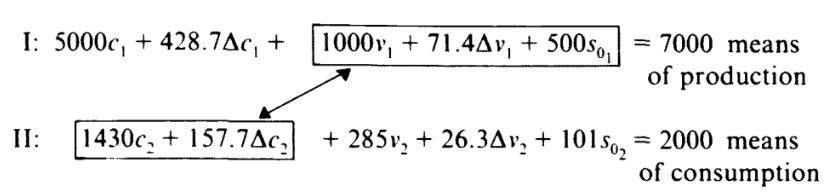
\includegraphics[scale=0.4]{rosha.jpg}
\label{fig:rosha}
\end{figure}

同样地,方框内的部分是两个部类之间相互交易的数量。第\Rnum{1} 部类为了满足其现有的
劳动力、计划增加的下一期的劳动力和资本家的消费,需要由第\Rnum{2} 部类提供1571.4单
位消费品,第\Rnum{2} 部类需要由第\Rnum{1} 部类生产的生产资料1587.7单位,用以补偿
当期消耗和计划中的不变资本的扩大所需的生产资料。这两个数字不等。“如果这是积累过
程的真实图景”,卢森堡推论说,“生产资料(不变资本)在第二年将有一个16单位的短
缺……同样地,消费资料将有16单位的过剩”,\textbf{这种不平衡将会逐期递增。}

卢森堡认为,无论是工人、资本家还是马尔萨斯主义者所说的“第三者”,都不能提供实现
剩余价值所必需的购买力。只有一个类型的消费者可以做到这一点:那些\textbf{完全外在
  于资本主义生产方式的消费者}。从而“在只由工人和资本家构成的社会里,为了积累而实
现剩余价值,就成为不可能的事情了。”存在“资本主义社会的生产能力与消费能力之间深
刻而根本的冲突。而这个冲突正是资本积累导致的,它周期性地产生危机,并驱使资本不断
扩大市场”。只有认识了这个矛盾,才有可能得出帝国主义理论。\textbf{马克思的分析无
  法揭示 “实现问题”的存在。它给人的印象是,资本积累可以不受限制地持续下去。从而
  放弃了“支持社会主义理论的最重要的客观论点……社会主义的政治行动和无产阶级阶级
  斗争的思想内容不再是经济事件的反映,社会主义不再是一种历史必然。}”《资本积累论》
的密码很容易地被解码:在批评马克思的同时,卢森堡事实上不仅批评了修正主义者,而且
还批评了考茨基和德国社会民主党正统的“马克思主义中心”。

卢森堡继续指出,在现实中,资本主义是“\textbf{通过不断地吸纳那些能够确保自身存
  在的条件来发展的}”。

卢森堡的帝国主义概念是很独特的。它不依赖于正式的殖民化,同希法亭强调垄断的增长或
银行支配地位上升也没有什么共同之处。\textbf{“资本积累的帝国主义阶段,意味着资本
  的世界竞争阶段,包含对资本落后地区——在那里资本曾经实现其剩余价值——进行工业化及
  资本主义的解放。这一阶段的特点是外债、铁道建设、革命与战争。”}卢森堡提到1900年
后向俄国、土耳其、波斯、印度、日本、中国和北非的大规模的资本输出。帝国主义的渗透
首先破坏了当地的农民经济,使得名义上独立的国家越来越依赖于欧洲的资本(该书第30章
以土耳其和埃及为例,对这个过程作了详细描述);然后,在这些迄今为止仍然落后的地区,
产生了不可抗拒的、要求独立发展资本主义的压力。这仍然是在暴力的背景下完成的:
\begin{quotation}
  经济上落后的国家及殖民地,通过战争与革命,获得资本主义自治。\textbf{革命在资本
    主义的解放过程中是必要的}。落后国家必须摆脱它们陈旧的政治组织,以及自然经济和
  简单商品经济的残余,\textbf{创造出一个适应资本主义生产目的的近代国家机器}。土耳
  其、俄国及中国的革命,即属此类。
\end{quotation}

这就引出了卢森堡引关于帝国主义的第二个定义,即帝国主义是“一个政治名词,用来表达
在争夺尚未被侵占的非资本主义环境的竞争中所进行的\textbf{资本积累}……(帝国主义)
在对非资本主义世界的侵略中,在相互竞争的资本主义国家之间发生的日益严重的冲突中,
变得愈来愈无法无天,愈来愈野蛮粗暴”。其表现之一就是\textbf{世界范围内对自由贸易
  的放弃},自由贸易“仅仅是资本主义积累史上的一个插曲”。表现之二就是\textbf{军国
  主义},《资本积累论》以对这个主题的分析结束。资本主义的每一个历史阶段都具有军国
主义的特征。军事力量被用于征服前资本主义地区,它也是“资本主义各国争夺非资本主义
文明地区的武器”。更重要的是,“\textbf{从纯粹的经济观点来看,军国主义是实现剩余
  价值的一个重要手段,它本身就是资本积累的一个领域”}。卢森堡重新回到再生产模型,
考察了作为消费者的国家产生的影响。她指出:“从工人所得中勒得的税收,在被用于军需
品生产时,就为资本主义积累提供了新的机会”,必须说明的是,卢森堡在这个问题中所作
的推理不很容易理解。

\section{对卢森堡的批判}
即使是同情罗莎·卢森堡革命左派观点的著述者,对她的经济分析也进行了猛烈的批评。
几乎没有人相信她试图证明的结论,即\textbf{在封闭的资本主义制度中积累是不可能的。}基
于同样的理由,人们对卢森堡进行一次又一次的批评,\textbf{资本家不但可以而且必须彼
  此互为客户},用于积累的那部分社会产品的需求,来自资本家意欲增加使用的不变资本和
可变资本。卢森堡对这类观点持有的反对意见,十分明显地表现在她对杜冈-巴拉诺夫斯基的
批评中,她同时也把对杜冈的批评用于反对布尔加柯夫和列宁的观点。\textbf{仅仅建立在
  资本主义需求增长基础之上,不存在对非资本主义市场的利用的积累,将意味着“人类消
  费变得越来越不重要,生产越来越成为目的本身”。}卢森堡认为,这种想法是荒谬的。但
她却错误地把持续扩大人的需求的目标,作为资本主义制度整体的目标。因为\textbf{资本
  主义制度的本质恰恰在于它的无政府性,资本主义没有也不需要一种目的,对资本主义进
  行任何形式的目的论的解释都是不恰当的。}在个别资本家层面上,卢森堡同样是错误
的。\textbf{资本家是被利润而不是被对消费增长的关注所驱动,}如果为了生产机器而不断
增加能够生产机器的机器生产是有利可图的,那就没有任何理由能够解释这种生产为什么应
当被中止。把无限制的均衡增长的可能性和它实际发生的可能性区分开来,当然是很重要的。
这里的关键问题在于投资的决定因素,但卢森堡对这一问题没有能作出详细说明。希法亭对
垄断作为一个限制支出因素的分析,有可能为这样一种投资理论提供必要的基础,但垄断在
卢森堡的思想中没有起到任何作用。

\textbf{总之,卢森堡混淆了个别资本的需要(需求的外部来源)和作为整体的资本主义制
  度的需要。}在卢森堡的分析中,还存在着三个更为严重的不相一致之处。首先,她对解释
经济危机的\textbf{比例失调论}做了猛烈的批判,因为(她认为)这一理论接受的是萨伊定
律,但她的批判据以建立的事实,她自己的解释也存在着和比例失调论类似的缺
陷。\textbf{在卢森堡提供的存在生产率提高的资本积累的算术例子中,消费品生产过剩的
  数量和生产资料供给不足的数量是相同的(如卢森堡自己承认的)。从总量上看,供给和
  需求是相等的。}第二,很难调和卢森堡对军事开支的分析和她对马尔萨斯主义者
的“\textbf{第三者}”的分析。\textbf{如果资本主义从把对工人征税所得的收入用于资助
  军备中获益,为什么用于国家闲职人员或国教方面的开支,不会产生像军备开支那样的效
  果呢?}很可能在\textbf{意识形态和政治}方面有很好的的理由,用于解释为什么资本主
义偏好于军事开支,而不是其它形式的国家活动,但卢森堡没有对这些理由进行解释。

卢森堡对帝国主义讨论的第三个也是最重要的不相一致之处,同向前资本主义市场出口的结
果有关,\textbf{如果这种出口被同等数额的进口抵消,那么出口就不会对需求水平产生任
  何直接的影响。只有出口顺差才能造成需求的净增加,但这必然意味着资本向前资本主义
  世界的输出(在不存在世界货币数量的增加时)。}卢森堡似乎没有意识到这里存在的难题。
在卢森堡的分析中,\textbf{需求不足}问题贯穿于整个资本主义发展的历史,但是资本输出
只在资本主义的最后阶段——帝国主义阶段——才变得重要起来,而且即便如此,资本输出也没
有产生像希法亭和列宁模型中所说的那种支配作用。在对资本输出的解释上,《资本积累论》
比希法亭《金融资本》的内容更少。\textbf{卢森堡的分析可以通过引入商品输出的间接影
  响来加以挽救,因为即使是在中性的贸易平衡的条件下,商品输出也会引致国内投资支出
  的增加。然而,这并不是卢森堡的观点,这再次表明卢森堡缺乏投资理论。}

此外,在卢森堡的观点中,还存在着布哈林在《帝国主义与资本积累》中指出的另外一
些不足。《帝国主义与资本积累》写于1924年,这部著作对卢森堡的理论进行了直截了当的
反驳,这部著作很可能是苏联打算对左翼反对派攻击时使用的(参见以下第十五章
)。\textbf{布哈林认为,在卢森堡的分析中,非资本主义的外围,实际上并没有受到资本
  主义的剥削,}它的功能只是实现在其它地方生产的剩余价值。此外,布哈林还认为,卢森
堡没有能够解释,为什么在资本主义努力寻求海外殖民地的同时,其本土仍然保留
着\textbf{大量的前资本主义经济形式}。布哈林还指出,卢森堡认为资本主义崩溃即将来临
的信念和她自己所持立场,在逻辑上也是不相符合的,因为世界上绝大多数人口仍然属
于“第三者”的范畴。

无论卢森堡的逻辑存在什么样的优缺点,她(完全不同于希法亭)在得出自己的结论时都是
毫不含糊的。她强调整个资本主义发展史中军事和国家力量的重要作用;强调军国主义和发
达国家之间日趋紧张的关系的经济必然性;她否定了封闭资本主义体制中稳定均衡增长的可
能性。在政治上,《资本积累论》是对德国社会民主党中的大多数人进行的激烈的、蓄意的
挑衅,因为无论是修正主义的右翼还是“马克思主义的中心”,都对消除危机的经济发展和
避免战争抱有希望。就像卢森堡在《反批判》中讲述的那样,党的机关报对《资本积累论》
持强烈的批判态度。令人惊讶的是,希法亭对《资本积累论》并没有作出反应,看起来可能
是他对经济争论失去了兴趣。考茨基迟来的反应,是以间接的方式进行的。当时,他把在
《新时代》上对这本书进行评论的任务,托付给了一个年轻的奥地利理论家——奥托·鲍威尔。
鲍威尔的文章的重要性,不仅仅体现在对卢森堡的批判上,而且也体现在他自己对马克思主
义危机理论的贡献上。

\section{奥托·鲍威尔的积累模型}

奥托·鲍威尔的分析是从对\textbf{人口增长后果}的思考开始的,他研究了在\textbf{充
  分就业情况下}资本积累必然发生的变化。这使得他能够对社会主义经济增长过程和资本主
义经济增长过程作出比较,在社会主义经济增长过程中,中央计划当局可以做出必要的调整,
而资本主义制度下生产缺乏有意识的社会调节。鲍威尔假定年人口增长率为5\%,不变资本的
使用每年以10\%的比率增长。这既包含了马克思资本有机构成不断提高的基本命题,也使得
鲍威尔能够对卢森堡提出的对再生产的分析必须考虑技术变化的挑战作出回应。“此时”的
鲍威尔,坚持剥削率保持不变,因此实际工资随着与资本有机构成提高相联系的生产率的提
高而增加。
\begin{figure}[H]
\centering
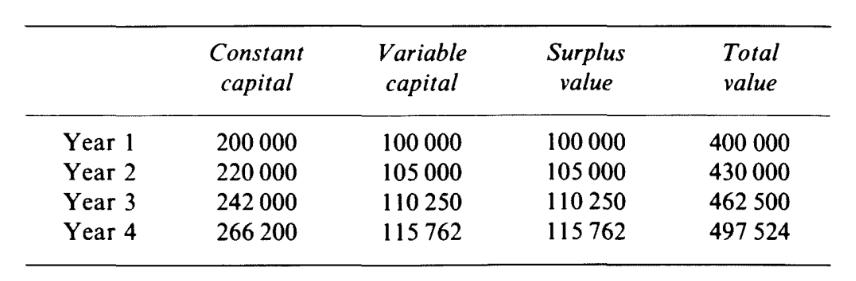
\includegraphics[scale=0.4]{bauer1.jpg}
\label{fig:bauer1}
\end{figure}

在这里,资本有机构成从第一年的2.00增加到第四年的2.30,利润率从0.333下降
到0.303(在剥削率一定的情况下,利润率必然下降)。每一年的净产出(即活劳动总量,或
者$v+m$)的增长率保持5\%不变。这是由鲍威尔的假定决定了的,由他的假定可知,可变资
本以每年5\%的比率增长,剥削率不变,因此剩余价值和可变资本有着同样的增长率。总产
出$c+v+m$以递增的比率增长,在第一年和第二年之间为7.50\%,在第三年和第四年之间
为7.57\%,更重要的是,鲍威尔称为 \textbf{“积累率”(一定程度上具有误导性)}的资
本家的储蓄倾向也在稳步增长。举例说,在第一年,100000单位总剩余价值中的25000单位被
留作积累,这使得资本家可以在第二年增加20000单位的不变资本和5000单位的可变资本。资
本家把他们收入中的25\%用于储蓄和积累。到第三年,这个比率上升到接近27\%,而且只要
不变资本比可变资本和剩余价值增长得更快,这个比率就会继续增长。

接下来,鲍威尔转向了对部类之间关系的研究。在第一年,可以表示如下:
\begin{gather*}
\Rnum{1} : 120000c_1 + 50000v_1 + 50000m_1 = 220000 \qquad 生产资料 \\
\Rnum{2}: 80000c_2 + 50000v_2 + 50000m_2 = 180000 \qquad 消费资料
\end{gather*}

如果资本家把剩余价值中的四分之一用于积累,并把它们完全投资在本部类,可以得出:
\begin{figure}[H]
\centering
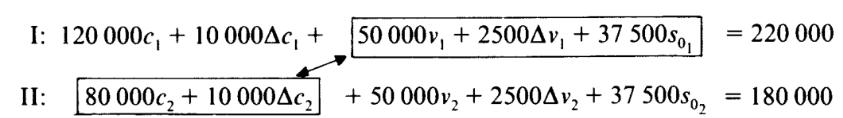
\includegraphics[scale=0.4]{bauer2.jpg}
\label{fig:bauer2}
\end{figure}
通过对方框内部分的比较,可以发现第\Rnum{1} 部类对第\Rnum{2} 部类生产的消费资料的
需求完全等于第\Rnum{2} 部类对第\Rnum{1} 部类生产的生产资料的需求(=90000)。但是
这不能建立两大部类之间的均衡,在第二年将出现如下情况:
\begin{gather*}
\Rnum{1} : 130000c_1 + 52500v_1 + 52500m_1 = 235000 \qquad 生产资料 \\
\Rnum{2}: 90000c_2 + 52500v_2 + 52500m_2 = 195000 \qquad 消费资料
\end{gather*}
生产资料产出的数量与鲍威尔假定的不变资本(是235000而不是242000)每年增加10\%所
要求的生产资料的数量相比,存在7000单位的欠缺,同时消费品的生产将会比必须的多出同
样的数量(是195000而不是188000),第\Rnum{2} 部类积累过剩,而第\Rnum{1} 部类则积累不足。

鲍威尔提供的解决方法是,第\Rnum{2} 部类的资本家把他们积累的剩余价值的一部分投资于
第\Rnum{1} 部类,增加第\Rnum{1} 部类的产出并相应地减少消费品的产出。在$10000
\Delta c_2$中, $5334$单位投资于第\Rnum{2} 部类中,剩下的 $4666$ 单位用于
第\Rnum{1} 部类的投资;同样地,$2500 \Delta v_2$中的1333单位用于第\Rnum{2} 部类,
剩余的$1167$单位转移到第\Rnum{1} 部类。第\Rnum{2} 部类的资本家可以通
过“或者\textbf{自己建立生产生产资料的工厂},或者通过\textbf{银行中介}把他们积累
的剩余价值的一部分转移到生产资料工业的资本家那里,供他们使用,或者购买生产生产资
料的公司的股份”来达到这一点。当然,第\Rnum{1} 部类的资本家的全部剩余价值被用于本
部类。

\begin{gather*}
\intertext{从而,第二年有}
\Rnum{1}: 134666c_1 + 53667v_1 + 53667m_1 = 242000 \qquad 生产资料 \\
\Rnum{2}: 85334c_2 + 51333v_2 + 51333m_2 = 188000 \qquad 消费资料 \vspace{1cm}
\intertext{第\Rnum{2} 部类的资本家拥有 4666c1+1167v1+1167m1=7000 单位的生产资料(除本部类的全部产出之外)。同样的推理,可以得出第三年的情况:}
\Rnum{1}: 151048c_1 + 57576v_1 + 57576m_1 = 266200 \qquad 生产资料 \\
\Rnum{2}: 90952c_2 + 52674v_2 + 52674m_2 = 196300 \qquad 消费资料 \vspace{1cm}
\intertext{以及第四年的情况:} 
\Rnum{1}: 169124c_1 + 61738v_1 + 61738m_1 = 292600 \qquad 生产资料 \\
\Rnum{2}: 96876c_2 + 54024v_2 + 54024m_2 = 204924 \qquad 消费资料 
\end{gather*}

与第一年相比,第\Rnum{1} 部类的资本有机构成提高了14.2\%( 从2.40到2.74),利润率下
降了9.18\%( 从0.294到0.267)。第\Rnum{2} 部类的有机构成提高了11.9\%( 从1.60增加
到1.79),利润率降低了7.01\%( 从0.385下降到0.358) 。

鲍威尔的结论就是:“不仅在第一年,而且在接下来的每一年,两个部类产出的总价值可以
在不受任何干扰的情况下出售,\textbf{总剩余价值得以实现}。因此,\textbf{卢森堡同志
  的假定——被用于积累的那部分剩余价值无法实现——是错误的}”。鲍威尔认为,并不是第一
年生产的全部剩余价值(如例子所显示的)都可以在当年得以实现有可能是正确的。如果资
本家只是在第二年开始的时候购买他们扩大生产所需的新机器,那么由 $\Delta
c_1+\Delta c_2$所代表的那部分第一年的剩余价值将只能在第二年得以实现;但它最终还是
被实现了。如果$\Delta c_1+\Delta c_2$ 所代表的商品是在资本主义世界之外的地方出售
的——卢森堡认为这是必须的——积累将受到损害,因为继续生产所需的生产资料将无从获
得。“这部分剩余产品从资本主义市场退出,将不会像卢森堡认为的那样使积累成为可能,
恰恰相反,它将使得任何积累都变得不可能”

在对卢森堡的观点做出分析后,鲍威尔转向对资本主义条件下\textbf{增长周期本质}的思考。
就这一问题来说,\textbf{必须放宽劳动力供给等于劳动力需求这一最初的假定}。如
果\textbf{可变资本的积累比劳动力的增长慢很多,将导致失业。}在这种\textbf{积累不
  足}的条件下,\textbf{实际工资下降,剥削率上升。}如果\textbf{在资本家的储蓄倾向
  既定的情况下,积累率将增大。最后到达的一点就是,可变资本的增长超过劳动人口的增
  长。然而,随后发生的是暂时性的积累过剩。}随着失业后备军的减少,实际工资再一次上
升,剥削率下降,这个过程一致持续到不仅利润率而且生产出来的剩余价值的绝对数量也开
始下降。马克思描述的“绝对生产过剩”导致一次重大的经济危机,在危机中积累受到严重
的限制,失业率上升,实际工资下降,利润率再次得到恢复。“繁荣、危机和萧条的周而复
始,经验地表现了一个事实:\textbf{资本主义生产方式自动地产生积累过剩和积累不足,
  资本积累反复地根据人口的增长进行调整}”。

一旦从\textbf{国际范围}内考虑问题,\textbf{国内人口的增长}就不再是一个关键因素。
积累过剩可能会因其它地方存在积累不足而在一些地区持续发生。
\begin{quotation}
  经常出现\textbf{积累过剩}的国家,把它们每年积累的剩余价值的很大一部分\textbf{投
    资到国外},而且这部分剩余价值越来越大。例如:法国和英国。经常出现\textbf{积累
    不足}的国家\textbf{引进国外资本并把劳动力输出}到国外。如东欧的农业家。在一国
  内部生产性资本的扩张总是受限于可以获得的劳动力。
\end{quotation}

这就凸显了卢森堡错误的帝国主义理论中的真理内核。\textbf{尽管积累在封闭的资本
  主义制度中是可能的,但它也受到了限制。帝国主义有助于放松这些限制,}它不仅通过扩
张能够招募到新劳动力的控制区,而且也通过获取原材料、刺激有机构成超过平均水平的产
业的发展,以及在经济危机期间,为“庞大数量的商品”提供市场来放松这些限制。

鲍威尔否认他的分析是对帝国主义的辩护:
\begin{quotation}
  因为在资本的辩护者想要证明积累——消费能力随着生产的扩大而自动地上升!——不受限制
  的本质时,我们揭示了积累受到的限制。在资本的辩护者想要证明普遍危机的不可能性时,
  我们说明了\textbf{积累的规律只能通过普遍的危机发挥作用},说明了危机造成的失业、
  工资的减少、大众苦难的增加、大多数工人日益增加的痛苦和愤慨。
\end{quotation}

从而,资本主义确实给自己带来毁灭,即使不是以卢森堡所假定的那种方式进行:
\begin{quotation}
  如果资本主义的扩张是可能的,它将会因军备竞赛、越来越多的压迫性税收、灾难性的战
  争而引起工人大众的愤怒。如果它的扩张被阻止了,对积累的限制就会加剧,危机变的更
  加频繁,持续的时间更长,更具破坏性……\textbf{资本主义将不会因实现剩余价值的机
    械的不可能性而崩溃,它将被它所激起的群众的愤怒所击败。}并不是只有当最后的一个
  农民和最后的一个小资产阶级都变成雇佣工人,从而不再提供一个实现剩余价值的市场的
  时候,资本主义才瓦解:被资本主义生产方式本身教育、联合和组织起来的日益壮大的工
  人阶级愈来愈强烈的愤怒,将会早得多地把它击溃。
\end{quotation}

\section{卢森堡的《反批判》}
鲍威尔的增长模型无疑是1914年之前由马克思主义经济学家尝试进行的\textbf{最成熟的宏
  观动态分析},它与现代\textbf{哈罗德—多马理论}之间的密切联系,直到最近才被完全理
解。鲍威尔文章的目的是为了驳斥卢森堡的崩溃理论,并说明\textbf{在封闭的资本主义经
  济中稳定的均衡增长是可能的}。尽管他对《资本积累论》的批评是有力的——这本来就是一
个很容易达到的目标,但是鲍威尔自己的模型也未能经受住更加细致的审查。早
在1929年,\textbf{亨利克·格罗斯曼}就证明了鲍威尔数值例子中所确定的增长路
径,\textbf{不可能无限期地持续下去},这已经被现代数学分析所证实。在经过32年的生产
周期后,\textbf{经济将会耗尽它用以维持给定的积累率提供资助的剩余价值}。这是鲍威尔
不变资本以两倍于可变资本的速度增加,剥削率保持不变的假设的必然结果。从代数上
看,m1和m2上升的太慢以至于无法满足模型所要求的 $\Delta c_1+\Delta c_2$ 的持续增加,
积累的过程无法一直继续下去。从技术上看,鲍威尔的模型过于武断。稳定增长只有在鲍威
尔提出的限定条件中,至少有一个被放松的情况下才是可能的。一个明显的选择是允
许\textbf{剥削率上升},从而可以增加用于积累的剩余价值的增长率。然而,即使在这种情
况下,\textbf{也不存在}充分的灵活性能够保证稳定增长的可能性,\textbf{确保这种可能
  性的最确定的方法是保持资本有机构成不变}。在不考虑鲍威尔本来意图的情况下,他的模
型是一种和技术变革过程中的\textbf{利润率下降趋势紧密联系在一起}(在任何简单的意义
上都\textbf{不是引起})的\textbf{资本主义经济崩溃理论}。

然而,这种判断完全不会损害鲍威尔危机理论的声誉,他的危机理论只能用它自身的优点来
加以评价。\textbf{积累不足时期和积累过度时期交替出现的概念有着直观的吸引力,}而且
它的确引起了许多后来的马克思主义经济学家的注意,这在很大程度上是因为它在避免了比
例失调、消费不足和利润率下降理论中的许多固有困难的同时,提供了对\textbf{周期性波
  动}的解释。但是,鲍威尔的理论也存在一个重大的缺陷,因为\textbf{它没有考虑生产能
  力利用率的波动。萧条时期总是产生严重的产能过剩,因为总需求不足以实现}经济中的生
产潜力得到充分发挥时生产出来的\textbf{全部剩余价值}。正是由于这个原因,马克
思\textbf{坚持把危机和实现问题紧密的联系在一起}是正确的。在文章的开始部分,鲍威尔
的确提到了资本主义社会生产能力的持续增加和资本主义消费能力逐渐缩小之间的矛盾,但
是,这种考茨基式的暗示并没有很好地加以深入展开。因此,鲍威尔对经济危机的解释是很
不完整的。

这些批评中,很少有哪个是由卢森堡在她那明显充满愤怒情绪的《反批判》中提出的,她对
鲍威尔提出的很多反对意见是\textbf{不着边际}的。她指责说人口变化不是资本积累的真正
基础,积累可以在人口保持稳定的情况下进行(就像当时的法国那样);\textbf{积累决定
  了人口增长率而不是相反}。 卢森堡把鲍威尔对两部类之间比例失调的分析驳斥为“纯粹
的欺骗”,并否认第\Rnum{2} 部类的资本家会像鲍威尔设想的那样,购买保持均衡增长所需
的4666单位的生产资料。这明显是错误的,卢森堡本来可以通过对平衡增长的可能是如何转
化为现实的进行提问,通过对直到\textbf{第二年进行购买之前一直保有第一年生产的商品
  存货的资本家的资金来源}进行探究,表现的更好。卢森堡认为鲍威尔模型中的\textbf{剥
  削率应当上升而不是保持不变},是建立在坚实的基础之上的,但即使是在这里,她也因坚
持在剥削率保持不变的情况下,“所有的技术进步只是为了工人的利益”而损害了自己的理
论。

虽然反对战争,但考茨基主义者拒绝接受通过革命推翻资本主义是通向和平的唯一的道路的
观点,他们认为能够使资产阶级相信帝国主义的终结是符合他们的利益的。“无产阶级和资
本之间为解决它们的世界历史矛盾而进行的最后的对抗,变成无产阶级和资产阶级之间
为‘\textbf{缓和}’资本主义国家之间的帝国主义矛盾而进行的\textbf{历史性妥协的乌托
  邦}”。正是因为卢森堡认为鲍威尔持有这样的立场,才对他的政治经济学如此敌视。


\section{考茨基对帝国主义的第二次思考}
考茨基1914- 1915年的文章和卢森堡的《反批判》,是最后的也是重要的论述帝国主义理论
的德国文献。

直到文章的最后部分,考茨基才开始和卢森堡(没有提到她的名字)背道而驰。在这里,考
茨基否认了帝国主义必然是资本主义的最后阶段。持续获得原材料和资本投资的出路,对资
本主义体系的生存是必不可少的。但是\textbf{军国主义和战争并不必然符合除武器生产商
  之外整个统治阶级的利益}。“今天,每一个有远见的资本家都会向他的同僚大声呼喊:全
世界的资本家,联合起来。”资本家们受到殖民地解放运动和国内工人阶级对帝国主义强加
给他们的财政负担的反抗带来的威胁,同时资本积累也因沉重的利税而处于极度的危险之中。
从而帝国主义在自掘坟墓……从纯粹经济学的观点来看,资本主义不是不可能再经历一个新
的阶段,即\textbf{卡特尔政策在外交政策上取得胜利的超帝国主义的阶段}。对于超帝国主
义,我们当然必须像对付帝国主义那样地同它作坚决的斗争,虽然它所带来的危险是在另一
方面,而不是在军备竞赛和威胁世界和平方面。

考茨基承认战争是可能的。因此,“\textbf{帝国主义的神圣同盟}”只能出现在全球冲
突终结的时候。任何世界战争持续的时间越长,这种同盟就越有可能产生。

作为事后诸葛亮,人们很容易对考茨基关于战争可能避免的主张嗤之以鼻。然而,在考茨
基写作的时候,存在着使人相信国际紧张局势正在缓和的理由。

战争爆发几个月后,考茨基重新回到这个论题,对修正主义者伦施和库诺进行了批评,他们
披着卢森堡的外衣,认为正是因为帝国主义是资本主义发展的一个必要阶段,所以社会民主
党对帝国主义的反对是无效的、反动的。考茨基认为这是对希法亭《金融资本》的误解,在
《金融资本》中,\textbf{帝国主义被认为是一种政策而不是一个独立的阶段}。因此,有可
能存在其它的政策选择,可以想象,\textbf{当前造成战争的政策将会被新的政策取代,这
  种新政策允许“国际上联合在一起的金融资本对世界进行共同的剥削”。这种超帝国主义
  政策将会削弱资本主义制度道德破产的趋势,预示着“资本主义的新希望和新期望的时
  代”。一切取决于战争的结果。}

\part{俄国到1917年的贡献}
\label{part:russia}

\chapter{俄国马克思主义的遗产}

\section{引言}
马克思留给俄国的遗产与留给德国社会主义者的遗产迥然不同。尽管他们能够接触到的马克
思的著作在本质上是相同的,但在\textbf{俄国资本主义不发达和沙皇专制的背景下},这些
著作中的有关内容显得较为晦涩。而且马克思关于俄国的具体观点往往没有什么充分的根据,
同他关于历史发展的整体理论毫不相干。

\section{俄国专制主义的本质}
以下将要证明的是,俄国作为欧洲持续时间最长的专制国家,在19世纪中叶仍然十分稳固。
沙皇国家中央集权官僚机构对社会统治的程度,是较早时期西欧专制国家无法比拟的。国家
是主要的土地所有者,拥有大部分的非农业经济部门。与幅员辽阔的领土相匹配,帝国控制
着一支庞大的军队,以及一整套对内镇压的国家机器。宗教不独立,教育机构的自治也微乎
其微。帝国的意识形态并不复杂,它打得旗号是“权威、正统和民族性”。这一意识形态的
谱系是清晰的、绝对的,因为沙皇专制国家没有经历过类似于在德国和奥匈帝国那样的改革。
俄罗斯帝国\textbf{完全不具备代议制议会、男性普选权和公民权}这些德意志帝
国19世纪70年代所具有的特征,甚至到了20世纪也依然如此。沙皇专制国家\textbf{经受住
  了}资产阶级革命的高潮和随之而来的拿破仑扩张的考验。事实上,它进行了反击,这种反
击不仅在最终击败拿破仑时发挥了作用,而且(自18世纪晚期以来)为了镇压革命和支持反
动势力而准确地打入西方。


俄国\textbf{“利维坦”(Leviathan)的阶级特征}是一个复杂的问题。现代历史学家往往
强调国家的独立和国家利益的至高无上。实际上,这种观点在马克思把俄国称作“半亚细
亚”国家时也有所体现。在革命之前,俄国马克思主义者也持这种观点。但是,马克思探讨
阶级与国家关系的理论蕴涵着复杂的视角。尽管现实是充满矛盾的,但这些矛盾并不是那么
的明显,人们不太可能就追求阶级利益所需的必要条件使达成共识。从而,任何一个阶级国
家都必定会获得某种程度的自治。

至19世纪中叶,经济上占统治地位的阶级是世袭贵族,他们的土地所有权是稳固的:
\begin{quotation}
  在大约100000个贵族地主中,接近50000个地主拥有不到270公顷地产。另外一半的贵
  族地主,却在10亿公顷贵族土地中占有97\%,而且在俄国的欧洲部分,这些面积超过了所
  有私人拥有的土地50\%多。给人印象更深的是,极少的(10\%)农业贵族拥有了2700公顷
  的土地,其比例占所有不动产土地中的75\%。甚至155个超级权贵,他们的不动产平均
  达270000公顷,其比例占所有贵族土地的33\%。
\end{quotation}
值得注意的是,国家机器与贵族结构的融合。在尼古拉一世统治下,
\begin{quotation}
  对应于国家官僚机构的级别,在贵族阶级内部形成了一种封建等级制。反之,凡在国
  家机构中占据确定位置的人,也被授予相应的贵族等级,在一定级别之上的等级为世袭等
  级。这样,一直到1917年,贵族头衔和特权,通过政治体制同各种级别的行政职能联系在
  一起。
\end{quotation}

这种相对单纯的封建专制主义形式,意味着支撑它的经济基础是极其落后的。1861年俄国的
人均国民收入不到德国、法国和意大利的一半,不及英国的1/4和美国的1/6。婴儿死亡率和
文盲率明显是欧洲最高的。

\textbf{国外的军事压力与国内的农民反抗和叛乱}这两股并行的历史力量,塑造了俄国社会,
这也是在稍后一个时期造成它分裂的力量。两种力量最初都起到了加强中央集权维护贵族安
全的作用,“\textbf{一方所需要的政治忠诚,是用满足另一方所要求的世袭农奴制换取
  的。}”这一过程(农奴制)开始于15世纪的相对较小的莫斯科公国伊凡三世时期,尽管与
所有的成长中的专制主义国家一样,专制主义在俄国经历了几番潮起潮落,但是,在18世纪
初彼得大帝统治时期,农奴制在更大范围内得到了巩固。独立的贵族权力受到了压制,通过
要求贵族承担普遍的服役义务,提高了贵族的官僚职能,同时也巩固了他们对农民的经济剥
削。农民流动受到限制,农奴制进一步得到强化,他们的反叛遭到镇压。城镇自治被粉碎了,
一个地理上不断扩张的帝国,为中央权力的高度集中创造了条件。

然而,随着资本主义工业化在西方世界的扩张,这一体制遭受的压力越来越大。
其\textbf{脆弱性},在1856年克里米亚战争失败中暴露无遗,此后,这个专制国家开始了更
大规模的现代化。19世纪60年代农奴制的废除和19世纪80年代以后凸现的对快速工业化的扶
植,是这一现代化过程中两个最显著的变化。前者为先前的工业化的加速发展,提供了更大
的活力。劳动力从农村向城镇的流动更为方便,国家和贵族之间分享农业剩余份额的竞争减
弱了。此时,国家面临的约束更少了,\textbf{从农村获取资源为雄心勃勃的工业化提供资
  金的能力更强了}。

到1914年,俄国已经成为世界第五大工业国,之前30年的增长超过了世界上其他任何地区。
一个高度发达的资本主义工业国在旧制度内得以建立。与此相伴的是,它造就了自己的掘墓
人——一个人数不多但高度集中的\textbf{城市无产阶级},这一阶级与农民有着千丝万缕的联
系,\textbf{对农民剥削的加重是这一过程得以完成的主要方式。}

\section{马克思和恩格斯论俄国}
这些不是马克思和恩格斯在19世纪40年代看到的俄国现实。很大程度上,他们所面对的只
是更为简单的专制政体。此外,19世纪70年代之前,他们的主要兴趣不在于帝国的内部条件
上,而在于俄罗斯帝国对外部产生的冲击上。

马克思和恩格斯论述亚细亚社会内部结构,即他们认为的同俄国有关的社会结构的更加深思
熟虑的著作,也是不充分的。事实上,\textbf{亚细亚生产方式}这一概念,现在被认为具
有\textbf{内在的不一致性},在把这一概念应用于经验研究时,时有不确切之处。就俄国个
案来说,这种情况并不是十分明显,这是因为人们经常通过为这个术语添加前缀而改变它的
限定条件。不管怎样,把沙皇帝国称为“\textbf{半亚细亚社会}”,只会使人更加困惑。在
这里,如同得到了一个加权平均的概念,但只对构成这一概念的某一单一要素作了详细说明,
而未对构成它的所有要素的权重进行设定。此外,马克思对俄国具有亚细亚社会性质的解释,
有时候显得有点过于唯心主义。马克思认为19世纪50年代之前,俄国没有“国内史”的观点
近乎荒谬。

恩格斯认为的沙皇政府在对内政策方面“不能理性行事”的观点,从根本上\textbf{低估了
  沙皇政府的自我调整能力}。

尽管如此,马克思和恩格斯通过把俄国与亚细亚生产方式联系起来,\textbf{强调俄国的非
  欧洲特征},这对后来的俄国马克思主义影响至深。在普列汉诺夫的理论发展中,他逐渐强
调俄国历史的非西方的特征(参见以下第八章),并且反对列宁的“\textbf{无产阶级和农
  民民主专政}”理论,因为实现这种民主专政,就\textbf{无法根除俄国农业秩序中的亚细
  亚社会的特征}(参见以下第十一章)。列宁本人也无法前后一致地提出一个有关俄国阶级
本质的理论,他在几种观点之间徘徊不定,\textbf{先是强调俄国的亚细亚属性,继而强调
  它的封建性,最后是它的资产阶级属性。}孟什维克则专注于在俄国复制他们认为的西欧政
治历史一直遵循的发展道路。托洛茨基最初形成的“不断革命论”的信念就在
于:\textbf{在俄国,国家创造了符合它自身利益的阶级等级。}在斯大林专制统治时期,作
为对“\textbf{一国社会主义}”意识形态进行广泛辨护的组成部分,\textbf{斯大林否定了
  亚细亚社会形态这一概念;这一概念和苏联现实之间存在的明显的相似性,使他感到不安
  (参见以下第十五章)。}

马克思关于1848年德国革命的著作,也以各种不同的方式影响着俄国马克思主义者。由于德
国经济的落后,马克思\textbf{起先承认}资产阶级领导革命是合适的,但很快他
就\textbf{开始批判}资产阶级的保守性。马克思最终转向了另一个立场,
即\textbf{强调}无产阶级和农民在激化革命方面发挥重要的作用。马克思预期的以这样的战
略成功的革命,到底是什么类型的革命,这并不太清楚。对1848年革命的研究,最终并没有
得出什么结论。马克思\textbf{随后集中关注的是发达资本主义国家背景下的无产阶级革命}。
不过,他确实从1848年革命中得出了某种具有一般性的经验教训,这反映在\textbf{德国马
  克思主义者在任何情况下都坚持无产阶级政党要保持自己的独立性上。}鉴于沙皇长期的专
制统治和俄国社会形态的相对落后,要求俄国马克思主义者\textbf{超越这一事实},并赋予
马克思对1848年革命进行的论述更加重要的意义是合理的。因此,普列汉诺夫不仅强调社会
民主党必须保持它的独立性,而且强调它要取得资产阶级民主革命的领导权(参见以下第八
章)。1905年之后,列宁在此基础上进一步提出,\textbf{农民的支持是必不可少的},在资
产阶级革命中无产阶级必将同资产阶级发生冲突(参见以下第十一章)。最重要的是,托洛
茨基主张,马克思有关1848年革命的观点,含蓄地表达了革命变革的一种新范式,在俄国存
在的由农民支持的无产阶级掌握革命领导权,意味着\textbf{资产阶级革命将迅速地进入社
  会主义革命阶段}(参见以下第十二章)。

马克思和恩格斯对俄国分析存在的缺陷,部分原因是由他们主要关注其他问题造成的。但是,
即使当马克思最终开始深入研究俄国的社会经济结构时,他的结论仍然具有“例外论”的特
征。他认真地考察了\textbf{以农民为基础的非资本主义发展的可能性},这种发
展\textbf{无需借助无产阶级的革命力量,最终达到社会主义。}在这方面,他深
受\textbf{俄国民粹主义}的影响。\textbf{民粹主义}是一场包含了多方面主题的运动,它
在整个19世纪后半叶主宰了整个知识分子阶层的思想。事实上,直到20世纪30年代,斯大林
的\textbf{集体化运动}才真正终结了民粹主义对俄国知识分子的影响。民粹主义也是一种中
介,马克思主义通过它开始在俄国发生影响,这一影响的核心部分就是马克思的经济学。

\section{俄国的民粹主义}

村社,在某些方面类似于原始共产主义。它的根本特征在于\textbf{公社土地的公有制},
土地在家庭之间定期进行平均再分配,以确保所有人维持生存。带状土地和轮作制农业使个
体劳动成为可能,但这要求农村公社进行\textbf{集中管理}。农民对领主费用和国家税收承
担连带责任,强化了这种特征,结果村社掌握并行使权力,村社权力约束了农民的个人主
义。19世纪60年代取消农奴制之前,农业经济自身及其同地主和国家之间的联系,是极
其“自然的”,几乎不存在货币交换。

因此,农村公社在多大程度上开始解体,农民在多大程度上开始出现社会分化,这些问题
在19世纪末成为俄国社会主义者争论不休的话题。事实上,即使是现在,这些话题仍颇具争
议。然而,农村公社以及维持其长期运行的惯例,并没有随着农奴制的消失而消失,这却是
一个不争的事实,而且非资本主义关系继续占据支配地位。这正是俄国农业极其落后、传统
残余对农民的意识仍在产生强大影响的部分原因。

这也为俄国的斯拉夫人捍卫旧政体提供了经济支柱。通常认为,村社阻止了西方常见的有害
的、堕落的个人主义的发展,因而也抑制了自由主义、无产阶级和社会主义的发展。相
反,\textbf{无论是否意识到,村社也把农民束缚于专制沙皇和东正教居于顶端的旧秩序
  中。}从而,俄罗斯帝国作为一个统一的国家,能够进一步地开拓疆域,能够“解放”南欧
的斯拉夫人,并与西欧的扩张主义相抗衡。

\textbf{对民粹主义者来说,正是村社提供了进入社会主义新社会的希望。}在他们的蓝图中,
村社关系阻止了西方个人主义的发展,奠定了(在他们看来的)现代社会主义蓬勃发展的基
础。从而,俄国在自身的发展过程中,\textbf{能够跨越资本主义发展阶段,通过对政治结
  构的适当改造,直接走上集体主义道路。}正是农业体制落后的社会本质,使得俄国的发展
可以是\textbf{直线型的——古老的俄国能够成为新俄国的基础}。资本主义发展的辩证法,既
不必要、也不值得期待。当然,民粹主义者认识到,村社并不是一种最优的社会制度。宗法
关系、近乎普遍的无知和经济的不发达如此明显,使得民粹主义的观点很难在具有浓厚的人
道主义精神、深受西方思想熏陶的知识分子阶层中流行。但是,民粹主义者相信,随着经济
的发展,沿着社会主义道路展开的启蒙运动,将会使这些不利因素逐渐消失。

马克思的经济学容易被融入到民粹主义的框架中。19世纪80年代之前,马克思的经济学主要
发挥了告诫功能:如果资本主义生产关系在俄国占据支配地位,那将会发生什么事情?换言
之,\textbf{俄国的广大民众将不得不经历伴随着资本主义的“运动规律”而来的所有的恐
  怖}。《资本论》对这些恐怖状况的描述,对它们和资本主义本质存在的紧密联系的分析,
对几乎所有的民粹主义思想家都产生了广泛而深远的影响。在马克思对民粹主义产生影响的
过程中,民粹主义也对马克思产生了影响。马克思没有试图去哄骗他的俄国读者继续接受
他30年来竭力阐述的观点,而是沿着采纳民粹主义思想的方向前进。

\section{“晚年马克思”}
马克思在赫尔岑的著作中初步接触到民粹主义思想,民粹主义并没有给马克思留下什么
好印象。这更多的是由于民粹主义者解释问题时表现出来的\textbf{斯拉夫气质}而不是他们
的内容造成的。无论是马克思还是恩格斯,他们从不掩饰对民粹主义作为俄国沙文主义的一
个变种的蔑视,尽管在他们看来,民粹主义可能更为仁慈。但是,后来的民粹主义者放弃了
斯拉夫主题,加之一系列其它因素的影响,19世纪70年代,马克思对民粹主义理解的视角发
生了转变。埃德蒙·威尔逊将这种转变描述为充满才智的头脑迸发出的“\textbf{最后的重要
  的火花}”,马克思这时\textbf{转变}了立场,承认俄国民粹主义者的奋斗目标是可能
的。20世纪的新民粹主义者坚持认为,在作出这种转变的同时,马克思本人也为“晚年马克
思”奠定了基础,新民粹主义者要求一并注意“青年马克思”和“成熟马克思”,“青年马
克思”探讨的主题极大地影响了一战后的西方马克思主义;“成熟马克思”的思想成为第二
国际的思想内核。

车尔尼雪夫斯基的经济学给马克思留下了深刻的印象,\textbf{车尔尼雪夫斯基强调俄国与
  西方的不平衡发展,认为俄国有可能复制西方的成就,而无需付出后者那种惊人的代价。}摩
尔根的人类学改变了马克思有关原始公社形式地位的观点,很可能促使马克思对俄国社会进
行了广泛深入的研究。

然而,“晚年马克思”并没有撰写出可与《1844年经济学哲学手稿》、更不要说与《资本
论》相媲美的著作。马克思只有一些晦涩的评论,散见于他为早期著作所写的附注中,以及
回答俄国一些向马克思征询对他们所关注问题的看法的信件中,事实上,这些信件的草稿有
些从来就没有发出。马克思有关俄国的观点,如果不借助现代的想象力加以扩展,所有这些
观点无论如何也难以构建成一个“体系”。这些观点,至多是一种梗概式的立场描述,这些
立场涉及的主题从未被详细地加以说明,也与早期的分析没有什么联系。

马克思个人对民粹主义的兴趣,最早出现在1877年他对民粹主义者米哈伊洛夫斯基关于《资
本论》的充满敌意的评论的回应中:
\begin{quotation}
  为了能够对当代俄国的经济发展作出准确的判断,我学习了俄文,后来又在许多年内
  研究了和这个问题有关的官方发表的和其他方面发表的资料。我得到了这样一个结论:如
  果俄国继续走它在1861年所开始走的道路,那它将会失去当时历史所能提供给一个民族的
  最好的机会,而遭受资本主义制度所带来的一切灾难性的波折。(《马克思恩格斯文集》第3卷,人民出版社2009年版,第464页。)
\end{quotation}

马克思坚持认为,《资本论》第一卷中\textbf{对原始积累的论述只适用于西
  欧},\textbf{否认}它是“一般发展道路的历史哲学理论,一切民族,不管它们所处的历
史环境如何,都注定要走这条道路”。它对俄国的适用性只表现在:
\begin{quotation}
  假如俄国想要遵照西欧各国的先例成为一个资本主义国家——它最近几年已经在这方面费了
  很大的精力——,它不先把很大一部分农民变成无产者就达不到这个目的;而它一旦倒进资
  本主义制度的怀抱,它就会和尘世间的其他民族一样地受到那些铁面无情的规律的支配。
  (《马克思恩格斯文集》第3卷,人民出版社2009年版,第466页。1857-1858年的《政治经
  济学批判大纲》表明马克思的前资本主义社会的发展方案并非线性的。)
\end{quotation}

1881年,在回复维拉·查苏利奇要求马克思提供关于“俄国农村公社可能的命运”的信件中,
马克思再次重申了这一立场。尽管马克思断言“这种农村公社是俄国社会新生的支点”,但
他又说“可是要使它能发挥这种作用,首先必须排除从各方面向它袭来的\textbf{破坏性影
  响},然后\textbf{保证它具备自然发展的正常条件}”。这种回复,明显地引发了马克思
更多的思考。至少有4封信件的草稿为人所知。正是这些信件充实了马克思论点的关键部分,
马克思认为,\textbf{农村公社把集体主义和个人主义结合到生产关系中。土地归集体所有,
  但劳动过程是个体式的,可转让的财产受制于私人交换。两种不同的发展都是可能的,}这
取决于哪一种要素占主导地位。沿着沙皇俄国的现代化启动的当前的道路继续前行,最终将
导致公社的消失和资本主义关系的产生。但是,这个过程并不是不可避免的。如果它因民粹
主义者的革命而中断,将有可能在公社的基础上建成共产主义,使西方资本主义的积极成果
融入社会主义者对公社进行的重组中。

在致查苏利奇的信件的草稿中,马克思没有再提及,\textbf{民粹主义发展道路的实现取决
  于西方发达国家的无产阶级革命}。然而,在为1882年俄文版《共产党宣言》所写的序言中,
他又加入了这一限定条件。这可能体现了恩格斯的影响,恩格斯是序言的共同作者,恩格斯
事实上起草了这一序言。同马克思相比,恩格斯有关“晚年马克思”主题的著述,无疑更加
强调西方政治领袖对实现民粹主义理想是必不可少的。也有证据表明,恩格斯从未认真地思
考过这一前景,即使是在马克思逝世之前。 1883年之后,恩格斯的有关这一立场的观点得到
进一步强化。恩格斯的怀疑论也反应在20世纪俄国马克思主义者的观点中。虽然他们有时候
承认俄国有可能避免经过成熟的资本主义的发展阶段,但是他们总是指出出现这种情况需要
国际革命。\textbf{“一国社会主义”学说是20世纪20年代的产物,1917年之后欧洲革命的
  失败是它形成的原因之一}(参见以下第十五章)。

对“晚年马克思”思想重要性的任何评价,都必须面对这种思想与早期著作中的思想的不一
致之处,而且必须考虑早期思想在19世纪70年代对马克思的影响。显然,晚年马克思的观点
与他早期的大量著述中反映出来的观点并不一致:马克思明显抛弃了在《资本论》中阐述
的\textbf{普遍适用的工业化的“自然法则”}。从他最早期著作开始,\textbf{一直存在的
  一个主题,即对无产阶级独自作为共产主义的代理人的效果的分析,现在加入了社会主义
  可以通过同知识分子和农民的结盟得以实现的新内容。}很显然,马克思早年许多有关农村
生活愚昧、农民的不开化以及缺乏政治上的可靠性的污蔑,适用的范围更为有限了。从19世
纪80年代开始,对西方帝国主义应当在更加相对的意义上加以认识,比如,\textbf{就西方
  帝国主义对印度的影响,马克思一方面谴责了它的残忍性,另一方面也欢呼其进步性。}

无论如何,民粹主义的目标都是不可能实现的。任何试图在村社的基础上实现的社会主
义,都将导致\textbf{独裁主义}。\textbf{领袖与群众之间的距离、劳动生产率的欠发达,
  都意味着不可能以民主的组织方式转向社会主义。}即使在农民中广泛存在着一定程度的巴
枯宁主义情绪,为了充分实现生产的社会化需要瓦解传统公社的生产关系,这势必要求解除
那些社会化的权力。那么,在避免经历阶级形成的沧桑巨变下,拿什么拯救统治精英?在马
克思逝世那一年,在青年马克思的马克思主义的指导下,普列汉诺夫明确地表达了这些用来
反对民粹主义的观点。“晚年马克思”当然没有为反对民粹主义的观点提供理论基础。

\section{结论}
因此,马克思留给俄国追随者的遗产,比留给德国同志的遗产更加复杂。德国马克思主义
者对马克思的亚细亚社会概念的理论兴趣有限。然而,对俄国马克思主义者来说,这个概念
表明他们面对的情况与欧洲完全不同。这突出了如下事实:\textbf{俄国资本主义的发展具
  有自己独特的特征,合适的革命策略需要采取特定的斗争形式},例如,马克思在评
价1848年德国革命时所概述的那些斗争形式。\textbf{即使是马克思成熟著作的核心部
  分——资本主义生产方式的运行规律——与俄国的相关性也是存在争议的。俄国不必等待修正
  主义的争论吞噬他们的各个阶层。从一开始修正主义就存在,而且明显得到了马克思自己
  的支持。}

\textbf{自1903年起},俄国社会民主党内部出现了新的裂缝。这时候,俄国社会民主党分为
孟什维克和布尔什维克两派。两派的分歧是由\textbf{党应当采取何种组织形式}的争议引起
的,但是后来把经济理论问题也牵涉进来(参见以下第8章和第11章)。如果不存在争议,也
就不会有俄国马克思主义的两派。\textbf{就政治经济学来说,最重要的是托洛斯基的不平
  衡和综合发展理论(参见第十二章)。}在\textbf{1917年之前},托洛茨基及其同仁接受
了\textbf{孟什维克的政党组织的观点},但是,他们的\textbf{激进主义}使得他们更像布
尔什维克的主要理论家列宁和布哈林(参见以下第十一章、第十二和第十三章)。1914年第
二国际解体后,俄国马克思主义的内部差异变得更加明显,不同团体进行了重组。1917年,
托洛茨基和列宁联合起来,但是大量的孟什维克和一些布尔什维克反对十月革命,因
为\textbf{他们认为冒险主义不符合正统马克思主义的原则}。(参见以下第八章和第十三
章)。

同时,由于马克思把俄国描述为欧洲的\textbf{反动堡垒},这使得俄国革命被认为是具有头
等重要性的国际事件。结果,\textbf{改良主义变成了一支微弱的力量,而革命强硬传统成
  为一支更为强大的潮流,}马克思本人体现出的这种特征,在说德语的理论家中只
有\textbf{罗莎·卢森堡}保持着这种传统。早期的经济理论的发展,清楚地说明了革命实践
的优先性。为了制定有效的革命战略,人们很少关注价值理论和资本主义危机理论,而把更
多的注意力放在理解俄国经济发展的本质上。

\chapter{普列汉诺夫的政治经济学}

\section{引言}
1880年左右,“晚年马克思”逐渐形成,年轻的普列汉诺夫却正在向着相反的方向发展。他
同自己过去的民粹主义决裂,接受了包含成熟马克思的核心主题在内的马克思主义,由此开
始了他的思想在俄国革命界逐渐占据统治地位的过程。他知道自己有关俄国的观点与马克思
的不同,而且在马克思逝世后的许多年,他很少得到恩格斯或其他马克思主义领袖的鼓励。
这些事实表明了他在知识方面的自信。……\textbf{孟什维主义}牢固地建立在普列汉诺夫的
马克思主义基础之上,没有任何一个孟什维主义理论家在学术地位上可以与他相比。……即
使在1905年普列汉诺夫同布尔什维克因“革命的算术”问题决裂之后,列宁仍然视自己为普
列汉诺夫革命的“代数学”的支持者(参见以下第十一章)。十月革命的胜利无法证明列宁
对普列汉诺夫哲学著作的赞赏,十月革命的理论原理与普列汉诺夫的理论格格不入(参见以
下第十三章)。在苏联,普列汉诺夫的著作,在官方认可的合法的基本的理论著作中,占据
突出的位置。

普列汉诺夫的马克思主义理论体系源自同革命的民粹主义的论战,他整个一生不断卷入各
种各样的理论争论。然而,他的纲领本身却表现出异乎寻常的恒定品性。实际上,普列汉诺
夫从来没有向他的论敌做过任何妥协。\textbf{俄国的资本主义将会继续沿着西方的道路发
  展,步入社会主义,要求马克思主义者首先集中关注资产阶级民主革命的实现问题。}

\section{普列汉诺夫体系,第二国际的正统和俄国马克思主义}
普列汉诺夫创造了一个术语——“\textbf{辩证唯物主义}”,用来界定马克思主义的本质。
在第二国际的知识分子中,他是马克思主义最博学的倡导者。他有关哲学思想的兴趣和知识
首屈一指。

普列汉诺夫的著作具有的这些特征,使得他的马克思主义被描述为一种具有极其僵化形式的
马克思主义,而且这主要还是一种\textbf{依赖于恩格斯晚期著作的马克思主义}(现在所知,
在始终不渝地支持这种马克思主义的人中,并不包括马克思),他的马克思主义也被描述为
一种能够十分便利地融入斯大林主义的意识形态中去的教条主义。毫无疑问,普列汉诺夫紧
紧地追随恩格斯,他无法认识到在恩格斯对黑格尔的分析中,以及把辩证法扩展到自然界时
存在的难题。普列汉诺夫也错误地认为,辩证唯物主义代表了一种存在内在逻辑联系的整体
性的世界观,对辩证唯物主义的批判必然出于某种无知或者出于某种反动企图。然而,下述
情况却是真实的,普列汉诺夫认为知识的探索具有至高无上的价值,他正确认识到不同形式
的折中主义的空疏无用,\textbf{准确地诊断出修正主义的本质——对正统的严重偏离}。更重
要的是,普列汉诺夫的体系不容易受到这样的指控,即他清晰地表达了一种机械唯物主义、
坚持了历史宿命论,或者说他\textbf{贬低了人的主体能动性}、强调了某种\textbf{政治寂
  静主义(political quietism)}。民粹主义批评家对他进行的批评正是基于这样的立场,
普列汉诺夫从不隐藏自己的反应。他对民粹主义的反驳,对理解作为整体的俄国马克思主义,
包括马克思主义政治经济学是至关重要的。

普列汉诺夫的个人兴趣更多地是在哲学思想上。这种情况表明了俄国马克思主义的一般特征,
俄国马克思主义作为一个相对独立的分支区别于中欧的马克思主义。1917年革命之前,技术
性的经济分析从来没有成为俄国马克思主义的重要组成部分。俄国经济欠发达的性质,使得
对价值范畴的讨论意义有限,\textbf{在第一次世界大战之前,俄国理论家关注的主要问题
  是理解资本主义兴起的意义,而不是分析它崩溃的原因。}确实,1914年前,俄国马克思主
义者在同民粹主义的争论中,就强烈反对那种认为资本主义根本没有辉煌的经济前景的观点
(参见以下第九章)。

普列汉诺夫不是历史发展道路的单线论者,不认为每个社会都必然要经过相同的发展阶段。
事实上,他得出了一个和马克思相同的结论:\textbf{从原始共产主义开始存在着不同的发
  展道路,在《政治经济学批判大纲》中,马克思对此作了概述。}当然,普列汉诺夫并不知
道马克思论述的内容,《政治经济学批判大纲》是在他逝世21年之后才出版的。此外,普列
汉诺夫努力为历史发展的多线论提供分析基础,与马克思的晦涩的评论相比,普列汉诺夫的
分析明显地要清晰得多。

普列汉诺夫在强调历史发展多线论时突出了三点:首先,\textbf{地理或自然条件}在决定经
济发展时具有重要的作用。正是这样的视角,使得普列汉诺夫能够解释俄国的半亚细亚、前
资本主义的社会条件,他相信,这样的社会条件致使俄国的历史与西欧的历史迥然不同。其
次,\textbf{构成任何一个复杂社会体系的经济的、政治的、文化的等子系统的相对自治}。
在这个基础上,普列汉诺夫认为,\textbf{人类意识和政治组织}在影响历史发展的过程方面
发挥了重要作用。最后,普列汉诺夫认为,\textbf{国际关系}对社会发展具有重大的影响,
对落后的社会来说更是如此。正是通过这种外部影响,俄国被推向了资本主义的发展道路,
《资本论》中描述的“运动规律”才适用于俄国。

自孟德斯鸠之后,人们已经认识到社会发展中地理因素的重要性。但是,普列汉诺夫的地理
决定论是独特的,这是因为它被整合进了马克思在《政治经济学批判》中总结的历史唯物主
义理论中。在普列汉诺夫看来,人类发展可以分为两大类型:\textbf{达尔文主义式的和历
  史唯物主义式的}。前者与物种起源有关,后者“\textbf{是从达尔文研究结束的地方开
  始}”的。在普列汉诺夫看来,正是不同类型的智人出现时的自然环境,决定了生产力形式
的最初发展。根据唯物史观,生产力代表了支配整个社会形态的关键因素,不同的地理条件,
在不同的社会形态形成上发挥了重要的作用。如果生产力有所发展——在普列汉诺夫看来,在
孤立的状态下,也有可能不发展——人类对自然的控制日益增加,减少了非社会因素在决定社
会发展方面的重要性。但是,\textbf{自然条件的约束作用从来不会完全消失,它只是与社
  会性的决定因素日益交织在一起。}

\begin{quotation}
  以往的全部历史,除原始状态外,都是阶级斗争的历史,这些互相斗争的社会阶级在任何时候
  都是生产关系和交换关系的产物,一句话,都是自己时代的经济关系的产物,因而每一时代的
  社会经济结构形成现实基础,每一个历史时期的由法的设施和政治设施以及宗教的、哲学的
  和其他的观念形式所构成的全部上层建筑,\textbf{归根到底}都应由这个基础来说明。
  (2009年版,马恩文集 第三卷 P544)
\end{quotation}
这使普列汉诺夫超越了恩格斯的“\textbf{归根到底}”(last resort)的原则,根据这一原
则,社会形态中不同因素之间存在相互作用,\textbf{经济因素}被认为是历史发展唯一的最
终起决定作用的因素。这里的问题在于,如果每一个因素都可以影响到其他所有因素,那么
我们就很难用\textbf{因果关系}的术语讨论问题了。因此,\textbf{如果说生产力的发展受
  上层建筑构成因素的影响,我们怎么能够又说前者决定了后者?}普列汉诺夫对\textbf{地
  理因素重要性}的强调,切断了这一循环。因此,他能够在接受所有的社会子系统相互作用
的同时,坚持包含着实质内容的一元论唯物主义。普列汉诺夫不厌其烦地强调,尽管发达的
科学不能忽视复杂性,但它也不能满足于任何一种二元论,也不能仅限于追溯不同要素之间
的相互作用。它必须寻求\textbf{有机的整体因果联系的基础}。

普列汉诺夫坚信\textbf{历史唯物主义},但他坚持认为,\textbf{自然条件或生产力的决定
  作用}的发挥,采取了中介形式,即\textbf{采取相对自治的社会关系的亚结构的中介形
  式}。只有在最原始的社会中,经济基础才直接决定上层建筑。\textbf{在更为分化的社会,
  经济基础的作用是通过阶级关系体系、政治权力和法律体系的结构发挥的。}为了支持这种
观点,普列汉诺夫深入研究了他认为的唯物主义的决定作用发挥的最不明显的领域——艺术创
造领域。

因为决定论是十分复杂的,所以社会发展的规律也是如此。但是,正因为如此,人类意识和
政治主体的能动性才有了发挥作用的空间。尽管普列汉诺夫从没有说明其界限,但
是,\textbf{他强调当有关社会发展规律的意识——主要是由马克思主义提供的——为了政治的
  目的被组织起来时,可能会对社会发展规律的运行产生显著影响。}在普列汉诺夫看来,这
说明在落后的社会,\textbf{社会民主主义}是如何与前资本主义社会条件发生联系的。它的
作用在于带来了\textbf{最有利于社会主义实现的资本主义的发展形式}。因此,分析实际产
生的是哪一种形式的资本主义发展?什么类型的资本主义发展是可能的?将会产生什么后果?
是政治经济学研究中头等重要的大事。正是在这些问题上,列宁、托洛茨基和布哈林以不同
的方式,最终与普列汉诺夫分道扬镳。在政治战略和战术层面,他们也不可避免地同普列汉
诺夫决裂了(参见以下第十一章、第十二章和第十三章)。

所有这些理论家都强调俄国资本主义面对的国际背景,普列汉诺夫的理论体系也是如此。
普列汉诺夫认为,如果没有西方世界那种发达的经济条件,俄国资本主义可能根本就不会出
现(参见本章以下第3节)。更一般地,他认为任何一个社会的发展轨迹,都深受它同其它国
家的联系的影响,特别是在这些国家处于不同的发展阶段的时候。普列汉诺夫不只满足于对
一种明显的方式的描述,这种明显的方式证明这种影响是真实存在的,而且努力去识别支配
这些相互作用的规律。正是基于这样的认识,他才在1917年采取了反对布尔什维主义的立场,
坚持认为只有孟什维主义才能为进一步的发展提供牢固的基础。这其中还蕴含着一个马克思
主义者对构成苏联建立原因的\textbf{政治经济学的批判}。

列宁和托洛茨基(尤其是托洛茨基)确保俄国社会主义革命取得胜利的战略,要求无产阶级
革命\textbf{扩大到更加发达的西方国家}。他们认为,只有到那时,俄国自身才能具
备\textbf{社会主义建设所需的充分的物质基础}(参见以下第十二章、第十三章和第十五
章)。但是,普列汉诺夫自己分析得出的结论,恰恰质疑了他昔日的追随者的这种逻辑。在
同民粹主义论战过程中,他被迫思考过类似的情况。民粹主义者有时也认为,欧洲更为发达
的经济条件,允许俄国绕过国内资本主义发展的成熟阶段,直接进入社会主义。普列汉诺夫
并没有立即否认历史的“\textbf{捷径}”是可能的。事实上,正像我们先前理解的那样,而
且在以下第3节和第4节,我们将会证明,普列汉诺夫自己的革命战略明确地取决于他的如下
信念:这些战略都是可行的,也都是合适的。但是,普列汉诺夫认为,在很大程度
上,\textbf{只有通过适当的关系结构的加速发展,它们才有可能实现。}它们不可能单纯地
依靠技术引进、资源转移或国际支持来实现。历史唯物主义包含了一种决定论的社会学理论,
普列汉诺夫慎重地对待它的术语。在社会主义革命的情形下,这意味着没有哪一个阶级能够
取代广大的、成熟的无产阶级。因此,在俄国,作为\textbf{社会主义必要的前提条件,一
  个充分发展的资本主义是无论如何也不可避免的。}如果革命领袖要在一个相反的假设下继
续前进,他们必然会逐渐削弱他们公开宣称的目标,而无论外部环境多么有利。

另一方面,普列汉诺夫自己的方案很明显以一种非常戏剧化的方式失败了。第一次世界大战
结束之后,布尔什维主义在俄国取得了胜利,改良主义和修正主义逐渐支配了西方的劳工运
动。普列汉诺夫\textbf{错}在哪里了?普列汉诺夫理论体系的本质特征,使得对该问题的回
答总是一个难题。困难源自普列汉诺夫对待辩证法的认真程度;辩证法赋予现实的丰富性掩
盖了普列汉诺夫的分析的局限性。比如,考虑到1917-1918年发生的事件,可以合理地假设,
普列汉诺夫的错误是因他对资本主义对俄国农民的影响的错误说明造成的,而\textbf{这个
  错误的根源可能在于依据马克思主义的范畴无法正确地理解农村生产阶级的本质。或者可
  以假设,即使是在民主革命时代,落后的资本主义的本质使资产阶级变成了反革命的力量},
尽管普列汉诺夫的战略要求他们成为一支\textbf{根本性的力量}。研究这些问题,对评价普
列汉诺夫的马克思主义至关重要,但是,由于他本人并没有意识到这些问题,致使这些问题
的最终解决变得格外困难。

\section{普列汉诺夫对俄国资本主义发展的说明}
普列汉诺夫认为,资本主义不会在每个国家以相同的方式出现,但即使如此,当资本主义
得到充分发展时,资本主义的“运动规律”却会在不同的国家以相似的方式运行。

俄国的西方化是由国家主导的“自上而下的革命”开启的。然而,在普列汉诺夫看来,这是
一个漫长的过程。直到19世纪60年代亚历山大的改革,同样是作为对国际事件的反应,才开
始为俄国的资本主义社会关系奠定坚实的基础。普列汉诺夫非常注意这些变化。在解释它们
的重要意义时,普列汉诺夫诉诸于商品经济的逻辑——他视之为社会变迁的一般经济规律。

绝对信守马克思对俄国的亚细亚社会的分类,是普列汉诺夫的一个弱点。这并不是因为普列
汉诺夫对马克思的盲从;普列汉诺夫的结论源自他对俄国历史资料的研究,这些历史资料无
论是马克思还是恩格斯都未能接触到,他对俄国社会具有重要的亚细亚社会性质的认识,随
着时间的推移而不断加强。

然而,任何情况都无法弥补这样一个事实:马克思的“半亚细亚”概念是\textbf{最不可靠
  的概念之一}(参见以上第七章)。

普列汉诺夫追随马克思,强调了商品关系在资本主义起源中的关键作用。再一次,他并
不是不假思索强调这一点的。在马克思对俄国进行的最后的讨论中,在证明了他民粹主义特
征的结论中,马克思的思考同样依赖于对19世纪60年代俄国改革所产生的效果的分析,普列
汉诺夫关注于这种情况。但是,普列汉诺夫不可能了解马克思的论述,因为马克思的著作直
到20世纪才被全部看到。更为重要的是,普列汉诺夫对这一方面的分析,比马克思对亚细亚
社会本质的评论更为有力。\textbf{商品生产}显然是资本主义发展的必要条件。但问题
是,\textbf{它是否是充分条件。}

马克思在《共产党宣言》中以一种最纯粹的方式强调了\textbf{交换关系}在资本主义起源中
的重要性。《政治经济学批判大纲》、《资本论》和“晚年马克思”的著作,都表明马克思
从来没有放弃这一思想。然而,他确实指出了商品关系作用的发挥存在的一些限定条
件。\textbf{马克思特别说明了商业资本和货币资本具有的两重性质。尽管这些资本形式既
  能够扩大商品流通,也能够加速小生产者的毁灭,但它们并不会引起生产方式的革命性变
  革。}恩格斯也指出,东欧的(第二次)农奴制拥有\textbf{融入世界市场的能力},马克
思对新大陆的奴隶制作出过同样的评价。从而设定了把市场生产和资本主义模式联系起来的
任何一种一般规律的限定条件。

普列汉诺夫忽视了这些限定条件,尽管在俄国农奴解放之前,使用农奴劳动的工厂强化了这
些限定条件,并且沙皇俄国1906年之前的农业政策有时候也确实是巩固了村社的地位,而不
是加速其灭亡。然而,我们很难指责普列汉诺夫在对俄国资本主义发展的实际讨论中也犯了
这样的错误。到19世纪末,沙皇专制很显然要求发展资本主义工业,而且如果不提高农业关
系的商品化程度,资本主义工业就不可能得到持续的发展。此外,既然19世纪60年代的改革,
迅速地改变了农业生产者的境况,因此可以期待它可能开启马克思所讲的资本主义发展
的“真正革命化的道路”。
\begin{quotation}
  从封建生产方式开始的过渡有两条途径。生产者变成商人和资本家,而与农业的自然经济和
  中世纪城市工业的受行会束缚的手工业相对立。这是真正革命化的道路。或者是商人直接
  支配生产。不论后一条途径在历史上作为过渡起过多大的作用一一例如17世纪英国的呢绒
  商人曾经把那些仍然是独立的织布业者置于自己的控制之下,把羊毛卖给他们,而向他们购
  买昵绒一一,就它本身来说,它并没有引起旧生产方式的变革,而不如说保存了这种生产方
  式,把它当做自己的前提予以维持。(资本论 第三卷 P373)
\end{quotation}

但是,普列汉诺夫把创建一支推翻沙皇专制的政治力量作为自己终生努力的目标。那么,他
为什么要相信革命将会推动资本主义发展的过程呢?况且,根据他的分析,沙皇专制推动了
资本主义的发展。对这一问题提供完整的答案,要等到下一节对他的政治理论的分析,但是,
普列汉诺夫对俄国资本主义发展进行的经济分析中存在的问题影响了他的政治理论。

普列汉诺夫(与马克思一样)表达出对农民的普遍的不信任。他对任何激进的土地革命的进
步性充满怀疑。毫无疑问,要求有一场肃清封建残余,\textbf{促进农村资本主义发展}的革
命。\textbf{在普列汉诺夫看来,问题在于“自下而上”的革命的实现,很可能会以其它方
  式阻碍资本主义的发展(比如,破坏大地产),同时提升农民的政治地位可能阻碍俄国的
  进一步欧洲化。}这些担忧是有充分依据的,尽管它们的实现形式与普列汉诺夫料想的有所
不同。在1917-1918年革命期间,俄国农民不仅明显地改变了先前引起农民分化的财产分配方
案,而且还\textbf{赋予村社以新生},这种特征直到20世纪20年代末的集体化时期才终
结。\textbf{在此意义上,农民革命具有极其退步的性质。普列汉诺夫没有考虑村社重新恢
  复的可能性},但是,这一事实不应当被看作是一个严重的缺陷。即使是对俄国农民问题有
更加深入研究的\textbf{列宁,在村社重新恢复变为现实的前夕,也没有看到这种可能性的
  端倪。}这是有关1917年的\textbf{最大的矛盾之一},即便是最敏锐的辩证学家都没有
预测到这个矛盾。但是,普列汉诺夫把研究的重点放在商品生产和资本主义的联系上,并没
有强调未来的发展前景,这种研究是直接用来反对民粹主义的观点的,民粹主义认为传统农
民经济组织有着持久的生命力。

普列汉诺夫对有关这个问题的另一方面的思考不是太清晰。他似乎曾经希望城市革命对
农村的支配达到这样一个程度,即\textbf{农业关系的改变将对资本主义发展产生最小的制
  约}。然而,他完全没有认识到,农业生产在经济方面所具有的独特本质以及十分有限的规
模经济。19世纪著名的资产阶级经济学家意识到这一要点,而马克思并没有认识到。然而,
德国的修正主义者强调\textbf{小规模农业继续存在的必要性},同普列汉诺夫一样,列宁尽
管也抵制修正主义,但他的著作却表明他学习了修正主义者(参加以下第十一章)。普列汉
诺夫则没有这样做。

与农业技术的特征相伴的是\textbf{独立的农民不同寻常的坚韧性},正是这种特征使得独立
的农民可以存活下来,并\textbf{阻碍生产的资本主义化}。在工业方面,市场的扩张使手工
业者成为商品生产者,并且城市的文化环境瓦解了这一过程中存在的传统束缚。商品生产关
系的资本主义化进展顺利,尽管有点残酷。农民则不同,农民在很大程度上自产自销,对他
们而言,“农村生活的愚昧状态”提供了更低的生产专业化的激励。\textbf{要不是货币化
  债务或税收给他们施加压力,农民就可以抵制市场的渗透,阻碍资本主义的发展。}

普列汉诺夫对沙皇专制下俄国农业发展的分析,体现了第二个方面的实质。他对19世纪60年
代的财政变化的集中关注,就完全与此一致。然而,他似乎并没有从一般意义上理解这一事
件,尽管他认为法国的历史很重要,在法国,革命的解决方式使得财政变化采取了另外一种
具体形式。\textbf{他非常忧虑“自下而上”的土地革命可能会阻碍其它地方的资本主义的
  发展。}此外,这些忧虑迫使他\textbf{反对列宁的“无产阶级和农民民主专政”的方案,
  该方案旨在充分挖掘农民的革命力量反对独裁专制,同时避免农民长期存在造成的影
  响}(参见下述第11章)。普列汉诺夫自己的方案未能很好地考虑这两个目标中的任何一
个。

另外,普列汉诺夫反对列宁的农民方案暴露了他分析中的另一个缺陷。\textbf{他对农
  业资本主义发展的分析集中于小生产者。他很少注意地主庄园的转变},他只是假设前者的
去自然化和去封建化将会影响后者,在更大的范围内使得后者资本主义化。这就忽视了庄园
主缺乏有效地调整自己经营行为的能力,和农奴制结束后庄园农业经历了一定程度的衰落的
事实。与此相对照,列宁认识到这一事实,而且这一事实巩固了列宁革命策略的逻辑基础
(参见第11章)。

\section{革命的结构}
因此,尽管普列汉诺夫坚持了马克思的政治经济学,尽管存在和他对沙皇专制下俄国资
本主义发展的理论分析相一致的证据,但是他的著作仍然存在重大的缺陷。要全面地认识这
些缺陷,我们必须转向普利汉诺夫尝试在他自己分析的经济基础之上构建的政治理论。对普
列汉诺夫的政治学的考察,将会进一步揭示他的经济学中存在的缺陷。

普列汉诺夫在他的著作的几个不同的地方,区分了“\textbf{革命的代数学}”和革命
的“\textbf{算术}”,这类似于战略与战术之间的区别。……他一直认为,同算术相比,代
数学是抽象的,因此坚持同一革命视角的人们之间可能存在重大的差别。正是基于这样的观
点,布尔什维克和孟什维克才可能长时间地认为他们同属于一个政党,即使当他们因为战术
的不同而决裂的时候也是如此。

普列汉诺夫为俄国革命者提供的“代数学”比较复杂。与国际社会主义者一样,他的最终目
标是世界范围内的社会主义革命。因为它会表现为一系列的民族的或地区的革命的形式,因
此世界社会主义革命包括俄国的社会主义革命。但是,普列汉诺夫认为,俄国的历史情况要
求进行作为\textbf{俄国社会主义革命必要的历史前提的资产阶级民主革命}。这是由俄国资
本主义欠发达的特征决定的,俄国资本主义的落后因对资本主义不利的专制环境而加剧。为
了取得资本主义最快速的发展,专制主义的政治的、法律的和文化的上层建筑必须被推翻。

尽管在普列汉诺夫看来,这样的一场革命将会开创\textbf{资产阶级作为统治阶级}的时代,
但他认为这样一个时代对社会主义的最终胜利是\textbf{必须的}。资本主义的加速发展将确
保生产力的发展,与此同时,资产阶级民主革命将为作为社会主义革命力量的工人阶级的发
展,创造有利的条件。工人阶级的人数将会增加,素质将会提高。为了文化的发展,剥削将
得到控制,民主自由将有助于组织的成熟。因此,无产阶级支持资产阶级革命符合自己的直
接利益和长远利益。

但是,普列汉诺夫认为,工人阶级在民主革命中充当资产阶级的副手并不是令人向往的事
情。尽管在反对沙皇专制的革命中,资产阶级有其客观利益,但是,它也会把革命限制在满
足自己的阶级利益要求的范围内。欧洲的历史经验证明了这一点。当资产阶级革命动员城市
大众反对旧制度时,\textbf{工人的直接收益是很小的,革命以一种不利于社会主义的未来
  的方式受到了制约。}尤其是在普列汉诺夫的早期著作中,他坚决主张,即将到来的俄国革
命不能再重复这种情况。所以,\textbf{无产阶级需要独立的政治组织来保护自己的利益,
  并推动资产阶级继续前进,否则的话,革命将会朝着其它方向发展。}他设想,资产阶级和
无产阶级结成反对专制的\textbf{同盟},但在这个同盟中,对专制制度的“共同”打击来自
于两个阶级\textbf{“各自”采取相应的行动},而且无产阶级应当成为同盟的\textbf{领导
  者}。无产阶级由此承担了“民族阶级”的角色。

尽管普列汉诺夫确信社会主义革命作为一个直接的目标是不可行的,但他也相信他所追
求的那种类型的资产阶级革命也是\textbf{不容易实现}的。他对俄国资产阶级日益增加的政
治保守性充满了鄙视。正如1905年和1917年的革命表明的那样,这些判断都是有事实依据
的。\textbf{普列汉诺夫的立场存在的缺陷,不是对资产阶级革命彻底性的盲目乐观,而是
  因为他把自己对资产阶级的理解仅限于政治行为层面造成的。}普列汉诺夫的战略的关键之
处在于,尽管资产阶级充满怯懦和犹豫,但是,它同专制政府之间存在着客观的、具有深刻
的经济根源的利益冲突。但是,普列汉诺夫从来没有深入研究过这个问题。在他的经济分析
中,他集中关注的是俄国资本主义在农业领域的发展。\textbf{他并没有对工业发展动力学
  进行过类似的分析,但他却赋予城市资产阶级革命的角色。}普列汉诺夫根据马克思的阶级
冲突的一般理论范畴和欧洲资产阶级的行为,审视了俄国的资产阶级。他没有从俄国工业化
面临的\textbf{具体的历史条件}出发创建理论,并在此基础上推导出资产阶级政治学。


如果他这样做了,那么,很明显的就会是,资产阶级在整个社会结构中占据的位置,会
使人怀疑它没有能力完成赋予它的那部分任务。经济中城市工业的比重相对较小,主要由国
家的军事需求和补贴提供帮助,由因沙皇政府实行严厉的财政政策而变得可能的国外资本的
大量注入推动产生的资本密集型产业占据了最重要的位置。此外,不太清楚的是,在工业与
专制政府之间是否存在根本的利益冲突,也就是说是否存在无法以进化的方式通过一系列的
妥协来解决的冲突。当然,工业资本会偏好更少独裁色彩的政体,扩大与政府的联系并推动
社会经济改革的进行。但是,在俄国,在1789和1848年引起资产阶级不满的问题,在很大程
度上是不存在的。\textbf{资产阶级对专制的不满与一个年幼的家庭成员类似,渴望发挥更
  大的影响,}但是,又囿于他一直以来成长于其中的环境。这正是列宁根据1905年革命得出
的结论;\textbf{他相信资产阶级赞同“普鲁士”式的现代化道路,即通过自上而下的方式
  重建旧制度,而无需推翻沙皇专制(参见以下第十一章)}。托洛茨基也得出了类似的结论,
但是,他更加乐观地认为这样的进化道路将会失败(参见以下第十二章)。与托洛茨基相比,
列宁对这种道路的前景的思考更为认真。

普列汉诺夫没有对俄国工业资本主义作出经济分析,因他分析农业资本主义时的一个重
大疏忽而变得更为复杂,这一点在前面的部分已经有所涉及。普列汉诺夫没有认识到,在制
约自由的农村劳动力市场的发展上,在确保农民中的很大一部分受制于不完全的土地所有上,
符合农村业主利益的经济基础的存在,也没有认识到非农民农业受到了政府财政政策特殊的
照顾。因此,\textbf{甚至是具有商业化倾向的地主,也仍然保持着对专制政府的依赖。}正
如俄国资产阶级无法复制18世纪末法国中产阶级的行动一样,俄国的土地所有者也不可能踏
上17世纪中叶英国农业资本主义的领导者选择的道路。在俄国,缺乏先前的资产阶级革命所
要求的经济基础,然而,普列汉诺夫的战略适合于他们政治上模仿的信念。

从而,\textbf{列宁认为的俄国现代化的“普鲁士式”的解决方法是建立在俄国社会的
  结构性因素基础之上的观点,是完全正确。}矛盾在于,这种情况在政治方面的表现在一定
程度上被普列汉诺夫证明了。他说明了从18世纪早期至19世纪晚期自上而下地进行的重建是
如何展开的。列宁看到但普列汉诺夫没有觉察到的是,1905年革命的结果预示了新的历史篇
章。\textbf{资产阶级的保守性深深地困扰着列宁,这使他断定彻底的民主革命将要求无产
  阶级与农民结成反对资产阶级同盟(参见以下第十一章)。此外,这样一种同盟不一定必
  然成功,另外的演化的方案正在形成,它可以“普鲁士式”的方式完成俄国向现代化的转
  变。这必然会在党的组织层面巩固列宁的布尔什维主义},列宁的立场确实可以在普列汉诺
夫对历史唯物主义中人的意识的分析中找到其理论基础。

列宁的战略填补了普列汉诺夫经济学中的另一项空白,尽管直到1917年,当促成他的革
命战略发生另一个根本性变化、并使他的立场更接近托洛茨基的时,列宁才意识到这一
点。\textbf{普列汉诺夫为资产阶级革命制定了两大目标:为资本主义的经济发展创造更有
  利的条件,为作为社会主义力量的工人阶级的发展创造更有利的条件。普列汉诺夫意识到,
  这两个目标在一定程度上存在冲突},因为资产阶级将会把革命局限于第一个目标;而工人
阶级将着眼于实现这两个目标。然而,至少是在1905年之前,普列汉诺夫不相信这是一个无
法解决的难题。\textbf{民主革命时期,资产阶级与无产阶级之间的冲突是第二位的;革命
  关注的是政治方面的问题,而非经济方面的问题。}有利于工人阶级作为社会主义的力量发
挥其未来的作用的彻底的改革(这些改革包括缩短工作日、最低工资立法以及对劳动过程的
管制等),并不是无法与资产阶级经济秩序的维持相适合。在这一点上,普列汉诺夫当然是
正确的,但是,\textbf{他没有认真思考的是,经济上与资本主义相适合的改革,将可能需
  要借助于政治上的改革来实现,也没有考虑政治方面的措施具有的经济方面的含义。}

根据普列汉诺夫的设想,无产阶级的领导权理所当然地包括两个方面:\textbf{无产阶级
  行使领导权,而资产阶级接受无产阶级的领导。}无产阶级领导权的获得,不只是无产阶级
行使领导权的问题。如果资产阶级抵制无产阶级(并且普列汉诺夫也充分认识到资产阶级有
兴趣这样做),将会出现发生第二次内战——在第一次内战中——的可能性,无产阶级将被迫行
动起来,既反对资产阶级,也反对专制统治。\textbf{无产阶级的成功将会产生重要的经济
  含义,因为物质生活将必然根据非资产阶级的原则来重新组织。}因此,寻求实现普列汉诺
夫“两阶段”革命方案中第一阶段革命的工人阶级,将\textbf{被迫超越这一阶段}。从这一
点看,普列汉诺夫对有关无产阶级为什么要让自己受限于资产阶级革命的观点的说明是不中
肯的。像批评家通常所指出的那样,问题不在于工人阶级将必然要求采取社会主义的措施,
而在于普列汉诺夫理解的属于“资产阶级”的措施引起了\textbf{政治上的冲突},而解决这
些冲突又带来了\textbf{新的经济秩序的变化}。\textbf{托洛茨基首先认识到普列汉诺夫的
  马克思主义中存在的这一问题,这个问题成为他的“不断革命论”的基础,在“不断革命
  论”中,资产阶级革命将嵌入在社会主义革命中(参见以下第十二章)。结果就是“革命
  的代数学”发生了戏剧性的变化。}

\section{结论}
普列汉诺夫有关为什么社会主义革命没有保证它实现的物质基础能力的观点,当然没有改
变。\textbf{如果没有大规模的资本积累、广大成熟的无产阶级和少量的农民,那么物质匮
  乏和反革命力量将会最终毁灭革命。在普列汉诺夫看来,“后发优势”或世界革命不可能
  颠覆正统马克思主义的这些基本真理。}

因此,普列汉诺夫把革命局限于资产阶级革命阶段背后的逻辑, 促使他走上了和列宁认为
的“普鲁士式”道路具有相同的客观含义的道路。(参见以下第十一章)。尽管普列汉诺夫
仍然坚持他最初的论述,但他实际上坚持的立场,在1905年革命期间和之后已经远离了他最
初的观点。工人阶级领导权的作用被淡化了,更加强调服从资产阶级的需要,而在帝国主义
战争中捍卫沙皇帝国也最终被认为是一种符合马克思主义的合适的立场。\textbf{普列汉诺
  夫退却的曲折道路是悲剧性的。它的根源,在“归根到底”的意义上,是他不能诊断出俄
  国资本主义落后的本质。}他的确正确地坚持了另一种极为愚蠢的“革命的代数学”,但是,
这一事实并不会减少它在这方面的失败。

普列汉诺夫体系中的内在矛盾,为即将在20世纪俄国革命运动中产生的分裂奠定了基础。
列宁、托洛茨基和布哈林各自提出了不同的方案,这些方案都是普列汉诺夫理论体系中最薄
弱环节清晰可辨的产物。实践也在发挥作用,因为作出修正,部分地就是运用普列汉诺夫的
马克思主义的结果,\textbf{更是普列汉诺夫的马克思主义无法应用的结果}。然而,尽管政
治战略至关重要,但是,每一个政治战略都依赖于资本主义发展的经济理论。

然而,在出现这样的理论之前,马克思主义必须首先在思想上取得胜利,民粹主义的社
会主义思想必须被击败。在这里,俄国资本主义的政治经济学又一次成为问题的核心。它是
争论的一个主要特征,尤其是争论引起了马克思主义经济学的发展,下一章将专门探讨这些
问题。

\chapter{19世纪90年代民粹主义和正统马克思主义}

\section{引言}
普列汉诺夫主要是在反对民粹主义知识分子的过程中,发展了他自己的马克思主义理
论。19世纪80年代,俄国工人运动欠发达的本质,使得普列汉诺夫的直接目标是
把\textbf{知识分子中的革命者}转变到他的立场上来,\textbf{而不是寻求对无产阶级的直
  接影响}。普列汉诺夫对民粹主义的批评,是马克思主义者在更广泛意义上对民粹主义批判
的一部分。第一轮批判是由恩格斯在1873年发起的,在俄国,同民粹主义的争论一直持续
到20世纪20年代末,这一争论随着斯大林集体化运动的兴起而结束。争论的高潮发生
在1894-1899年,当时,批判性的出版物的数量显著增加。这一时期,也是马克思主义的社会
民主主义思想取得知识上突破的时期。特别是在在一系列成熟的反对观点的攻击下,作为民
粹主义哲学基础的经济理论被削弱了。

\textbf{观念的胜利有其物质基础。19世纪90年代}初,俄国的广大农村地区遭遇饥荒,这不
仅进一步激化了这一时期的论战,而且表明农业经济陷入深重的危机之中。随后几年,工业
迅速增长,城市无产阶级作为一支政治力量及时地出现了,这进一步支持了马克思主义的观
点。很显然,资本主义正在发展,\textbf{无产阶级的激进与农民的逆来顺受}形成鲜明的对
比。因此,普列汉诺夫的马克思主义原理得到了具体的证明;随着民粹主义队伍的衰落,社
会民主主义的队伍逐渐壮大。

胜利并不全面,民粹主义改头换面地幸存了下来,这反映了普列汉诺夫理论体系中存在
弱点。非马克思主义的社会主义者尽管难以表述清楚,但他们认识到,落后的资本主义的本
质并不完全像普列汉诺夫描述的那样;在俄国,资本主义的充分发展存在重大的障碍,马克
思主义理论对农民行为的分析是不充分的。当20世纪资本主义开始“东扩”时,当马克思主
义和农民扮演了重要角色的反殖民运动开始结合起来时,民粹主义开始复仇。民粹主义特有
的主题重新出现在新的背景下,马克思主义的发展受到极大的影响。在这一意义上,在第七
章讨论的“晚年马克思”思想方面存在的不足,并不是一个致命的缺陷。20世纪下半叶,民
粹主义作为一项世界性政治运动,同1914年之前为俄国正统马克思主义提供理论基础的“成
熟马克思”的思想相比,\textbf{更接近于马克思主义}。

\section{民粹主义的俄国资本主义理论}
民粹主义的观点包罗万象,\textbf{只在敌视资本主义发展、主张社会进步以俄国经济生
  活的传统制度为基础的意义上,它们才构成统一的整体。}至于“进步”的确切内涵、实现
它的最佳方式、资本主义在多大程度上构成了一种威胁,以及非资本主义制度的健康状况和
适用性问题,都是莫衷一是的。但是,在19世纪最后20年间,民粹主义理论的一致性逐渐增
强。一般认为,俄国资本主义发展受到了阻碍,全面仿效西欧不仅是不合适的,而且也是不
可能的。如果俄国要作为一个主权国家生存下来,那么经济演化主要地必然表现
为\textbf{非资本主义式}的。其他类型的出路将导致俄国从属于西方国家,甚至可能沦为它
们的正式的殖民地。

民粹主义的重要理论家有V·沃伦佐夫和N·F·丹尼尔逊。他们每个人都运用马克思主义经
济学理论原理,特别是丹尼尔逊,他把《资本论》翻译成俄文,而且在差不多30年时间内,
同马克思和恩格斯保持通信联系。实际上,他把自己视为一个马克思主义者,人们也普遍认
为确实如此。然而,他和沃伦佐夫所做的,就是\textbf{整合马克思主义经济学与民粹主义
  的主题},以此支持民粹主义。正如我们在以上第七章看到的,这是民粹主义著述家的一贯
特征。而且当他们的观点遭到社会民主主义反对时,他们往往倾向于扩大对马克思和恩格斯
的批判,但是,大多数民粹主义者仍然对马克思主义的奠基者持有好感。令普列汉诺夫懊恼
的是,民粹主义者通常视俄国“正统”马克思主义是不合法的,是错误的。

尽管沃伦佐夫和丹尼尔逊在诸多重要问题上存在异议,但在关于俄国资本主义不可能得
到充分发展的观点上,确实可以放在一起,并一同加以考察的。他们的理论基础是相同的:
资本主义生产关系必然引起\textbf{消费不足}。从而,纯粹形式的资本主义将陷入停滞;只
有资本主义社会关系的外部因素,才能消除停滞、促进增长。\textbf{剩余价值不可能在一
  个完全资本主义化的经济中实现。因为剥削率为正,工人的消费需求不足,而且消费不足
  不可能由资本家的消费去消除,因为剩余价值的一部分被用于积累或储蓄。为了确保剩余
  价值全部实现,资本主义经济需要一种特定类型的市场体制——存在着源于外部消费需求的
  市场体制。}

这是资本主义的\textbf{一般理论},它没有分析作为资本主义变种的俄国的\textbf{具
  体缺陷}。但是,民粹主义经济学家却将一般理论应用于俄国,否认俄国资本主义能够开辟
外部消费需求的充足来源。\textbf{俄国的“后发”,意味着国外市场已经被更为发达的国
  家所垄断。}民粹主义者认为,俄国资本主义只能通过沙皇政府财政政策的人为刺激,以一
种退化了的形式得以维持。最终,即使是对这种寄生现状的维持来看,国家的资源也是不足
的。如果不抛弃照搬西欧策略的话,那么持续的、全面的经济发展就不可能。俄国必须走不
同于西方国家的特殊道路(但是,也许可以借鉴在一些非资本主义国家可以使用的现代技
术)。

关于俄国经历的资本主义发展的实际后果,民粹主义经济学家之间存在分歧。沃伦佐夫
强调,农民进行“\textbf{人民生产}”的能力,可以抵御侵蚀和保持农业的完整性。与此形
成鲜明对比的是,丹尼尔逊则指出了资本主义对农业经济的毁灭性影响。在他看来,资本主
义产生的是\textbf{毁灭而不是转型}:\textbf{农业生产者日益贫困化但却没有转变为雇佣
  工人}。他进一步论证,\textbf{内在于资本主义部门的技术进步,提高了资本有机构成,
  因而减少了对劳动力的需求,提高了财富的集中程度。因此,任何发展都是内向的,但非
  资本主义经济并没有转化为一种新的生产方式。}

特别是丹尼尔逊的观点,可以被解释为《资本论》中政治经济学的“特殊案例”,这也
是他自己理解《资本论》的方式。\textbf{丹尼尔逊的理解强调了马克思分析中存在消费不
  足的线索,回避了发展中存在的矛盾。}相反,正统马克思主义强调和发展了民粹主义者忽
视的马克思主义政治经济学中的那些原理。普列汉诺夫最早清楚地表达了所有可以用来反击
民粹主义的主要观点。这一事实本身就是一个非凡的成就,如果考虑到普列汉诺夫的内容写
于《资本论》第二卷和第三卷公开出版前这一事实,那更是如此了,《资本论》第二卷和第
三卷的内容对正统观点的形成是至关重要的。但是,在19世纪90年代的“大论战”中,普列
汉诺夫把扩展和完善民粹主义者早期经济学批判的任务留给了他人,自己则集中精力反对民
粹主义理论中的哲学和社会学原理。

许多能力不同的著述者,以不同的方式阐述了正统马克思主义的经济学观点。许多人认
为需要详细浏览整个争论过程的批驳性材料,但结果发现这些材料中存在大量的重复和夸张
的成分。然而,我们可以挑出两位参与者,他们明显地胜过他人。杜冈-巴拉诺夫斯基和列
宁以一贯的——其他人只是偶尔能够达到的——\textbf{专业性和彻底性},表述了正统马克思主
义对民粹主义的批判。\textbf{杜冈-巴拉诺夫斯基的理论集中证明,通过扩大生产资料再
  生产实现剩余价值具有可能性。列宁强调,剩余价值的实现内在于资本主义关系的粗放式
  增长之中。}杜冈-巴拉诺夫斯基的经验分析充实了他的理论分析,因为正是\textbf{俄国
  工厂的发展}支撑了他的理论框架。列宁的经验研究也与自己的理论视角相吻合:他以迄今
为止无与伦比的系统化程度,记录了\textbf{农业经济中生产关系的变化}。杜冈-巴拉诺夫
斯基和列宁的主要观点是\textbf{互补}的。不存在一方否定了另一方要点的情况,而且两个
人通常用自己的方式对这两个问题做出自己的说明。在专业领域,他们各自做出了自己的贡
献,我们在以下四节将集中分析这些内容。这与许多作者的做法不同,他们强调19世纪90年
代批判民粹主义的论战中司徒卢威的重要性。司徒卢威作为“大论战”的催化剂和社会民主
主义中自由力量的一位重要组织者,无疑是十分重要的。但是,在政治经济学方面,无论同
杜冈-巴拉诺夫斯基还是同列宁相比,他都只能算是二流人物。司徒卢威在反击民粹主义的
主要经济观点时,对他的对手作出了重大的(和错误的)让步。

\section{杜冈-巴拉诺夫斯基论扩大再生产}
杜冈-巴拉诺夫斯基首先认识到1885年出版的《资本论》第二卷提出的马克思再生产模型
的重要性。在他看来,这些模型是经济理论上迄今唯一的最重要的成就,因为它们提供了一
个严谨的框架,借助于这一框架,可以对资本主义不同经济部门之间各方面的相互联系作出
具体分析。1894年,杜冈借助于再生产模型,提出了\textbf{周期性经济增长理论},批判了
其它的理论,并且对英国的经济波动进行了经验分析。在这一过程中,他清晰地批判了所有
的\textbf{消费不足论},其中包括民粹主义的消费不足论。作为对其他理论的替代,他强调
要把“\textbf{比例协调}”以及它的反面“\textbf{比例失调}”作为理解资本主义运行的
关键。

马克思主要以数字例子的方式,阐述了再生产理论。在方法上,杜冈效仿马克思,但是,
他把马克思分别论述的三个部分整合为一体首先,他常常加上一个第\Rnum{3} 部类(尽管为了达到
同样的效果,马克思有时候也把第\Rnum{2} 部类分为生产工资商品的部类(\Rnum{2} a)和生产奢侈品的部
类(\Rnum{2} b));其次,更为重要的是,杜冈把资本有机构成的提高引入他的分析中;再次,至
关重要的是,杜冈强调资本主义生产是\textbf{为利润进行的生产}。生产的目的不是为了满
足人类的需要,也不是为了满足\textbf{消费需求或推动经济增长}。如果出现了这些情况,
那它们就只是\textbf{派生的结果},而不是\textbf{最初的目标}。当然,没有哪个马克思
主义者会不赞同最后一个观点(或者事实上包括后面两个观点),但是,杜冈-巴拉诺夫斯
基认为,他们并没有体会到它们的真正内涵:正因为如此,消费不足论才在马克思主义中获
得了一定程度的认可。杜冈认为,一旦经济分析结构得当,消费不足论的核心部分就是无效
的:\textbf{资本主义经济中的矛盾,只有通过造成生产部门之间比例失调的因素才能加以
  解释。}

这在一定程度上坚持了马克思分析再生产问题时的结论,马克思认为只要生产部类保持必
要的比例关系,剩余价值的实现就不成问题。第Ι部类产生的对消费品的需求,实现了
第\Rnum{2} 部类的剩余价值;与此相类似,第\Rnum{2} 部类对不变资本的需求,使得第Ι部类生产的剩余
价值得以实现。加上资本有机构成的提高,\textbf{这就意味着资本主义的发展,本质上可
  以被视为生产资料的进一步生产是为了生产资料的生产。}尽管从人类价值的视角看,这种
观点似乎有些荒谬——并且杜冈-巴拉诺夫斯基承认它的\textbf{荒谬}之处,但是,从这种分
析中必然得出对资本主义生产的正确理解。\textbf{它也意味着剩余价值的实现越来越独立
  于消费需求。}杜冈-巴拉诺夫斯基通过设想一种\textbf{(虚拟的)自动化经济}——在该
经济中,大量的机器的生产只是为了用来生产更多的机器——把这种推理方式的逻辑推至(或
几乎推至)极端。同样,在达到这一终点的过程中,伴随着的是消费下降而导致的剩余价值
实现困难——可能是大量人口的贫困化。因此,在资本主义的运行过程中,消费需求并没有起
到什么特殊的作用。

对于沃伦佐夫和丹尼尔逊极端形式的消费不足论,杜冈-巴拉诺夫斯基作了有力的驳斥。但
是,许多马克思主义者拥护的更合情理的消费不足论(参见以上第四章到第六章和以下第十
章)并没有受到损害。杜冈的模型只是认为,并不存在像民粹主义宣称的那样的必然的、持
续的国内消费需求不足。积累周期性的中断导致暂时性的短缺,仍然是可能的。当然,他承
认,\textbf{可能引起危机的某种类型的比例失调,可以被描述为消费不足。}然而,事实上
他并没有强调这一点。\textbf{他认为,资本主义经济机能失调的根源,在于缺乏确保按比
  例安排生产的制度。}杜冈-巴拉诺夫斯基强调了比例失调的一般现象,而非消费比例失调
的可能性,并且逐渐地反对各种形式的消费不足论。此外,他坚持认为,\textbf{即使人们
  可以把消费不足论正确解释为经济危机的原因,消费不足也不必然带来停滞。}杜冈-巴拉
诺夫斯基在他的周期理论中就试图证明,\textbf{资本主义经济中存在诸多能够确保经济繁
  荣的力量。因此,俄国资本主义并没有受到阻碍;俄国走西方国家此前走过的同样的发展
  道路,并不存在什么障碍。}

杜冈-巴拉诺夫斯基的观点是抽象的,但用它来消弱同样抽象的民粹主义观点的基础却是合
适的。然而,他并不总能认识到自己的结论的局限性。\textbf{特别是马克思的再生产模型,
  是根据价值向价格转形前的价值范畴建立的。因此,生产价格和利润率并不能明确地加以
  描述。}在这里,杜冈-巴拉诺夫斯基同马克思一样,\textbf{没有能说明资本主义经济中
  的价格—利润结构可以原则上引导资本家走上他所描述的增长道路}。 今天有可能做到这一
点,但是,杜冈并没有进一步深入阐释自己的观点(即使是在《资本论》第三卷出版之后)。
更重要的是,考虑到杜冈-巴拉诺夫斯基写作时的背景,\textbf{他的模型没有能准确地描
  述资本主义经济实际遵循的经济增长模式。}例如,他承认\textbf{对外贸易}在英国资本
主义扩张过程中发挥了关键作用。但是,他是根据具体的情况来分析这一点的,而不是从理
论上对它进行解释。在殖民扩张的高潮时期,这是一种极端的和戏剧化的立场。马克思主义
不可能长期满足于从偶然事件的重要性的角度来解释帝国主义,正因为如此,杜冈-巴拉诺
夫斯基的著作受到了批评。就俄国资本主义的具体情况来说,杜冈-巴拉诺夫斯基的观点也
并非无可挑剔。\textbf{再生产模型事先已经假定发达资本主义经济的存在。但是,部分民
  粹主义者讨论的情况是俄国资本主义受到了更大的非资本主义部门的阻碍。}列宁认识到这
一缺陷,他在论述实现问题时采取了与杜冈非常不同的视角。但是,同杜冈-巴拉诺夫斯基
一样,为了消除民粹主义思想残留的最后一点合法性,列宁也采用了一种极端的方式来阐述
自己的观点。

\section{列宁关于通过扩大商品生产实现剩余价值的理论}

支配列宁的观点的是一种\textbf{广义的发展阶段类型},这种发展从自然经济开始,经过商
品生产阶段,最终进入社会主义社会。城乡分裂、不同性质产业的出现、经济活动的专业化
和劳动分工,这些都等同于商品生产的增长,资本主义商品生产是商品生产的更高阶段。每
一个阶段的生产同前一个阶段相比都更有效率,而竞争是一个阶段取代另一个阶段的推动
力。

在列宁看来,沃伦佐夫和丹尼尔逊的致命错误在于,他们没有认识到\textbf{资本主义不
  发达阶段}的性质。把资本主义等同于大规模的机器工业集中于城市中心、只使用雇佣工人,
它们关注的只是资本主义的最高阶段,忽视了多种原初形态的资本主义与发达类型的资本主
义并存的事实。列宁认为,\textbf{正确地看问题,就要求承认资本主义关系可能采取多种
  形式。而且他还指出,一旦资本主义关系稳固地建立起来,商品生产(从而资本主义商品
  生产)就不可能受到阻碍。当然,它们不可能受到有限市场的限制,因为这一过程能够确
  保市场按相同的步调,随着经济的发展而发展。}在这里,列宁借助丹尼尔逊自己的观点反
驳丹尼尔逊。\textbf{当商品化和资本化的过程确实带来贫困化时,这一事实本身必然包含
  着市场的扩大。}生产者的生产资料被剥夺,一无所有的生产者被迫为购买消费品而出卖劳
动力。\textbf{一方面市场扩大了,另一方面大量的生产者贫困化了。}

列宁没有忽视伴随着资本主义发展而带来的贫困问题,他的分析也不是简单化的。他并
不是没有解释资本主义的早期形式有时可能会阻碍其向更为发达的形式发展。\textbf{较高
  的发展阶段甚至可能以不同的方式部分地恢复过去的经济组织类型。}他完全承认,并不是
所有的产业都会遵循同样的演化模式,并且那些法律认可的自然经济的残余,可能会阻碍经
济的发展。因此,很难指责列宁不关心他所设想的社会发展过程的复杂性。

另一方面,列宁以一种极端的形式来应用自己的原理。从本质上说,普列汉诺夫尽管持有同
样的看法(参见以上第八章),但在具体应用时,他较为谨慎。因此,普列汉诺夫
把\textbf{资本主义}看作是\textbf{商品化过程的结果},而列宁则倾向于把两
者\textbf{等同}起来。\textbf{他视“国内市场发展的程度”为“国内资本主义发展的程
  度”},结果“关于俄国资本主义国内市场如何形成的问题,就归结为下面的问题:俄国国
民经济的各个方面如何发展,并朝什么方向发展?” 1900年,斯科沃尔特索夫在对《俄国资
本主义的发展》的评论中批评了列宁,因为列宁把两者混为一谈。这是一个重大的缺陷,我
们将在这一章的第7节回到这一问题。

\section{《19世纪的俄国工厂》}
《19世纪的俄国工厂》首次出版于1898年,该著作追溯了自彼得大帝时期开始的俄国工业的整
个发展过程,仅在这一点上,就对民粹主义经济学家研究重点中的诸多内容作了有力驳斥。
但是,这部著作的内容超越了19世纪90年代的论战,它到目前仍然是\textbf{在历史唯物主
  义框架下对工业化过程分析的最好的著作之一。}

杜冈-巴拉诺夫斯基主要关注的是要削弱下述观点的基础,这种观点认为,俄国政府在发展
工业生产时发挥的作用,赋予工业一种“人为的特征”。他雄辩地证明,发端于彼得大帝时
期的\textbf{俄国的现代化是生存的必然选择}。正如我们在以上第八章看到的,普列汉诺夫
持有同样的立场,但杜冈-巴拉诺夫斯基给这种观点增添了更多的内容,并且更加详细地解
释了它的经济特征。他特别强调,这一阶段体现出来的资本主义的部分特征是不可避免的。
新型生产必须在\textbf{大规模工厂}中进行,以便有效地利用进口技术。\textbf{仅商业资
  本家拥有资源和能力来筹办新工厂。}由于提供自由劳动力的国内市场并不存在,因此,国
家有必要进行直接干预,以提供强制劳动。

杜冈-巴拉诺夫斯基解释说,随着时间的流逝,发展的辩证法将会越来越明
显:\textbf{那些有利于工业增长的措施成为进一步发展的障碍。}债役劳工最初促进了发展,
但是,随后又变成了一种障碍。雇佣工人日益增加,农奴制改革的压力增大。然而,他承
认,\textbf{19世纪60年代解放农奴的运动阻碍了一些大工业的发展。}那些严重依赖农奴的
工厂不得不做出改变,开始了痛苦而又漫长的——最终证明是有效率的——重组过程。在杜冈-
巴拉诺夫斯基看来,大工业的发展并不是马上就取代小规模的手工工场。在许多情况下,产
生了相反的效果。最初局限于工厂的生产,因为需要引进劳工的技能,于是就转向了小生产
者,并造成了传统工业活动的复兴。此外,随着工业生产的发展,随之增加了供给商的活动,
而这些供给商有时是按传统方式组织起来的。但这只是有可能,因为商业资本长期以来已经
主导了许多老的工业。接着,杜冈-巴拉诺夫斯基指出,机械化破坏了家庭式生产,尽
管——正如爱尔福特纲领所表明的——不存在“小规模”生产直接被“大规模”生产所取代的情
况。

杜冈-巴拉诺夫斯基认识到,“\textbf{后发者}”的发展模式明显地与英国的模式不同,
而民粹主义经济学家则往往把英国作为分析的基准。\textbf{后发国家的工业化缺乏自发性:
  国家行为发挥了支配性的作用,非资本主义制度与资本主义关系结合在一起,公开的强制
  补充了市场训诫,技术引进发挥了重要作用。同样的,西方的意识形态与传统信念相连接;
  特定类型的阶级利益重新塑造了自由主义。即使如此,他强调,俄国工业资本主义的发展
  意味着整个俄国经济日益融入世界市场。所以,民粹主义支持的“特殊道路”变得越来越
  无关紧要;实际上所走的道路已经把俄国融入到整个欧洲的经济史中。}俄国西方化的过程
仍在继续,而且在这个过程中维护了国家的主权,尽管是借助历史的、特有的方式实现的。

杜冈-巴拉诺夫斯基因而成为第一个认识到“\textbf{后发国家}”与英国模式存在显著
差异的社会主义者,而马克思本人和民粹主义者则把英国提升到典型的地位。此外,正是杜
冈-巴拉诺夫斯基指出的“\textbf{不平衡与综合发展}”的思想,为托洛茨基不断革命论提
供了唯物主义的基础。\textbf{不断革命论认为,无产阶级革命可能首先在落后的俄国社会
  发生,而不是在发达的西欧这个中心发生。}与普列汉诺夫和集中关注俄国农业资本主义发
展的列宁不同,托洛茨基同杜冈-巴拉诺夫斯基一样,集中研究城市工业。但是,他又与杜
冈不同,他根据工业化对社会结构的影响,考察了俄国工业化的“现代性”问
题。\textbf{托洛茨基认为,俄国的工业化形式显著地扩大了俄国无产阶级的规模,同时又
  使集中在城市的国内资产阶级和小资产阶级人数减至最少。在与国家发生任何冲突时,无
  产阶级将成为主导的力量;同样的,无产阶级的阶级利益也成为最重要的事情。}此外,沙
皇时代鼓励工业发展的方法使农业问题恶化,这使得城市革命可以利\textbf{用农民的支持}。
正如现在已被广泛认识到的,托洛茨基的理论与任何一个他的竞争对手的理论相比,都更加
准确地说明了1917年革命的\textbf{阶级动力学}(参见以下第十二章)。

杜冈-巴拉诺夫斯基并没有深入研究托洛茨基基于与《19世纪的俄国工厂》相同的经济视角
推导出的这些政治问题。杜冈的观点是直接用来反对民粹主义的,他更加强调俄国现代化的
独特模式,将使俄国未来的历史与西欧的历史一致。杜冈-巴拉诺夫斯基相信,俄国融入世
界市场,使得民粹主义者偏爱的“特殊道路”已经不可能实现。在这一点上,他是正确的,
但是,在民粹主义在理论上失败之后,他所概括的不同的“\textbf{特殊道路}”具有的革命
含义,为1917年布尔什维克政治学的一个重要分支奠定了基础(参见以下第十二章和第十三
章)。

\section{俄国农业资本主义的发展}
杜冈的许多观点因列宁著作中的官方的证据而得到加强,但杜冈却从这些官方的证据中得
出完全不同的观点。在20世纪的发展过程中,列宁这位未来的布尔什维克的领导人非常接近
于这种观点,并且远离了支配了他自己19世纪80年代的分析的观点。列宁对杜冈的观点进行
了改造,从而产生了与杜冈本人的立场完全不同的政治行动。(参见以下第十一章、第十二
章和十三章)。这在前面已经有所提及。在与民粹主义论战达到高潮时,列宁仍然坚信他自
己的理论愿景,坚持自己的经验证明。他关注的主要是农业经济问题。\textbf{列宁的主要
  目标是想从经验上证明“人民生产”中的不平等与小生产者的分化——这两者明显的——都是
  资产阶级和无产阶级两极分化的症状。}在19世纪90年代晚期,可以得到的统计资料远远超
过普列汉诺夫15年前可以接触到的统计资料,而且列宁仔细地运用这些资料,对民粹主义经
济学发起了猛攻。

在本章第5节讨论的列宁理论的本质,为他完成自己的任务提供了大量的机会。对资本主
义的发展有多种衡量指标;\textbf{作为一个过程,而非终结状态,资本主义可以视为一种
  无所不在的力量。}列宁充分地利用这一点证明,不只是使用雇佣工人,有官方证据的专业
化和商品化、土地所有者的不平等、生产资料的集中所有这一切,都表明了资本主义的发展。
他并没有宣称\textbf{农村的小生产者实际上构成了典型意义上的资产阶级和无产阶级},只
是说存在非常确凿的证据表明这种转化正在进行。为此,他集中分析了\textbf{农民家庭}而
非个人情况的变化。农村的无产阶级主要由贫困的农民家庭构成,那部分无法获得足够的生
产资料的农户被迫使他们家庭中的一些成员进入劳动力市场。在另一个极端,富裕的农民家
庭不能提供他们自己生产活动中所需的劳动力,而不得不雇佣工人。因此,形成了一种与马
克思在《资本论》第一卷中阐述的(英国)方式\textbf{不同的资本原始积累机制}。列宁并
没有强调这一点,他承认,仍存在\textbf{大量中等农民家庭},他们既不受雇于他人,也不
雇佣其他人。然而,他坚持认为,大量的资源被富裕的农民拥有所产生的激烈竞争,将逐渐
使农户转变为资产阶级和无产阶级。因此,\textbf{“人民生产”会逐渐转变为资本主义生
  产,尽管它只是发生在资本主义的低级阶段。}

农村的这样的阶级构成,说明了民粹主义的观点为何能够流行。在列宁看来,民粹主
义——正确的(即根据马克思主义范畴)可以理解为——只不过是\textbf{小资产阶级的意识形
  态}。它反映了大量农民家庭被边缘化的境况,进一步的经济发展将使农民家庭进一步衰落。
但是,这是危险的,因为它妨碍了无产阶级阶级意识的形成,并且民粹派推动的改革可能会
成功地阻碍更高形式的资本主义的发展。

但是,列宁并不认为民粹主义是完全反动的。他认识到民粹主义对资本主义的反对同
它\textbf{对封建主义的敌视}是类似的。在俄国,农奴制当然早就废除了,但由于农奴解放
的不彻底,许多封建残余保留了下来,结果确实需要一场反封建的农民革命。对农民自愿转
让和获得土地与劳动力的能力的制约、劳动租金的长期存在,市民自由权的缺乏,所有这一
切都阻碍了经济的发展。就民粹主义对这些问题采取的批判性立场而言,它是一种客观的进
步力量。因此,同许多其他的马克思主义者(包括普列汉诺夫)相比,列宁对民粹主义对手
的态度显得更加复杂。尽管他赞同,民粹主义的思想是错误的;但他也认识到,民粹主义对
社会民主主义运动可能是有用的。事实上,这些思考在列宁的思想中注定要发挥更大的作用。
但是,在它们发挥作用之前,列宁已经彻底地修正了他自己有关俄国资本主义发展的理论。
我们将在第十一章中考察这一变化。

\section{马克思主义观点中存在的一些问题}
19世纪90年代,民粹主义的经济理论被削弱了,在马克思主义批评家的抨击下,民粹主义的
哲学和社会学也同样遭到削弱。这并不让人感到惊讶。正统马克思主义是一个更为优越的思
想体系,而且经济发展的主要突破也符合马克思主义的论述。然而,我们还是可以找到正统
马克思主义中存在的严重缺陷。这些缺陷中的一部分,事实上就内在地存在于马克思主义自
身,而且它们在思想史中一再明显地暴露出来。

\textbf{“实现”和“国内市场”问题是一个供给和需求的问题:需求是否足以吸纳供
  给?但是,无论是马克思还是他的俄国追随者,都没有能够准确地使用这些范畴。}马克思
自己论述的内容是自相矛盾的。他既坚持新古典的需求概念,\textbf{排除任何需求不足的
  可能性};又提出另一个(凯恩斯主义的)需求概念,\textbf{认为需求不足是长期的}。
在解决这一问题时,俄国的马克思主义者止步不前。列宁似乎完全没有意识到这一问题的存
在,因而在对《资本论》晦涩的内容引用时,遇到了困难(参见以下第十章)。杜冈-巴拉诺
夫斯基认识到需要一种需求理论,但他自己的分析甚至连马克思的水平都没有达到。因此,
他们的理论缺乏坚实的基础。今天,这些理论可以在坚实的逻辑基础(当然,这和他们经验
研究的有效性并没有什么联系)上被重建,然而,他们的对手的观点问题更多。但是,这并
不意味着可以不予理会对马克思主义的观点的批评,在同民粹主义者的论战中,这种批评认
为马克思主义的观点并非是确凿无疑的。

其实,鉴于沙皇时代工业化的实际历史情况,部分地接受民粹主义分析的精神而不是它的具
体内容,还是可能的。19世纪90年代,俄国工业资本主义的发展实际上是存在矛盾
的。\textbf{扩张所需的资源,并不完全来自国内生产的剩余价值,}就像杜冈-巴拉诺夫斯
基抽象的再生产模型所描述的那样。\textbf{它们部分是通过对农民经济地榨取以及维持有
  利于这种榨取的村社制度提供的。这阻碍了土地生产率的增长,因而也抑制了进一步增加
  对农村的剥削以继续这一过程的可能性。}这一问题的严重程度仍不清楚,但是,马克思主
义者显然没有充分地认识到这一问题。在此意义上,沙皇时代工业政策的核心部分存在“人
为”的因素,民粹主义经济学家比马克思主义者更加明确地强调了俄国的特殊性。

对俄国农民和更为一般的农村小生产者的研究,至少为民粹主义的直觉提供了进一步的
支持。我们在以上第八章指出,普列汉诺夫对资本主义发展的分析存在两个缺陷:它没有注
意到农业领域规模经济的相对缺乏;它忽视了农民可以利用的维持自身地位的手
段。19世纪90年代,俄国马克思主义者重复了这一错误。事实上,列宁的错误比普列汉诺夫
的更为严重,因为他把资本主义发展等同于市场的发展。此外,再次同普列汉诺夫一样,俄
国马克思主义者并没有认真地思考俄国农业领域具体的经济组织,对俄国经济发展和农民分
化产生的限制。正如列宁所坚持的那样,村社并不只是其经济基础已完全被商业化破坏了的
日趋没落的封建残余。它在技术上也发挥了必不可少的作用: 轮作的敞田制要求一个管理机
构凌驾于个体农民家庭之上,而且把农民的份地分开也存在巨大的经济上的困难,更不要说,
法律方面的约束一直维持到1907年。因此,村社根植于当时农业经济的现实,而不只是在过
去才如此。

此外,尽管农民的经济活动产生了收入和财富上的不平等,但这些不平等的程度
是\textbf{有限的},并不必然导致农民之间的\textbf{阶级差别}。引起农民分化的因素之
一与农民家庭的生命周期、他们的再分配程序以及村社的再分配过程有关。商品生产的发展,
并不总是与这些实践相冲突;它可能推动而非阻碍它们作用的发挥。因此,列宁的理论观点
和他对经验资料的重构,最轻意义上也是误解了农村的可观察到的不平等。\textbf{农民比
  他认为的更具同质性,并且把它视为小资产阶级阶层的理由也是不充分的},因为这样做,
反映了对农民可能采取的政治和经济行动的一种过于狭隘的观点。当列宁把俄国农民同马克
思在《路易·波拿巴的雾月十八日》一文中描述的法国农民进行比较时,他的错误就更为明显。
对这一点的具体证明出现\textbf{在1917-1918年间,村社制度不仅没有被农民革命削弱,而
  且成为完成革命的一种手段,而且因为革命的成功而得到加强。农民既不是一种资产阶级
  力量,也不是一种无产阶级力量,也不是这些力量的混合物。}在现有的马克思主义范畴中,
没有哪一个与它相吻合。

所有这一切,并不意味着民粹主义经济学本质上是符合实际的。显然不是。但是,它的
确意味着,并不像马克思主义者倾向于认为的那样,对民粹主义的批评和对马克思主义的证
明是同一项任务。的确,列宁的分析最容易受到指责。没过多久,他就认识到自己著作中的
不足之处,尽管他从没有解释过19世纪90年代他自己的错误的确切性质(参见以下第十一
章)。但是,当这十年结束时,他做出\textbf{改变}的可能的原因是非常明显的。正在他试
图用官方资料证明农民内部的阶级形成时,俄国马克思主义本身正在经历分化的过程。特别
是出现了一个与德国类似的修正主义派别。\textbf{为阻止修正主义的不良影响,列宁有关
  农业经济学的立场发生了微妙的变化,}而且这很可能进一步导致了他在20世纪初对自己的
策略进行了重大的调整。当然,这并非俄国修正主义唯一的、重要的意义。作为对马克思主
义经济学的一种批判,它是值得关注的,更不要说它也体现了一种真正的分析层面的洞察力。
这将构成下一章的主题。








%%% Local Variables:
%%% mode: latex
%%% TeX-master: "../main"
%%% End:
